\documentclass[11pt, a4paper]{article}

\usepackage[utf8]{inputenc}
\usepackage[ngerman]{babel}
\usepackage[T1]{fontenc}
\usepackage{amsmath, amssymb, amsfonts, amsthm}
\usepackage{geometry}
\geometry{a4paper, left=2.5cm, right=2.5cm, top=3cm, bottom=3cm}
\usepackage{hyperref}
\usepackage{titlesec}
\usepackage{enumitem}
\usepackage{setspace}
\usepackage{booktabs}

\setstretch{1.15}
\titleformat{\section}{\large\bfseries\sffamily}{\thesection}{1em}{}
\titleformat{\subsection}{\normalsize\bfseries\sffamily}{\thesubsection}{1em}{}

\newcommand{\mvec}[1]{\boldsymbol{#1}}
\newcommand{\cl}{\mathcal{C}\ell_{3}}
\newcommand{\clc}{\mathcal{C}\ell_{3}(\mathbb{C})}
\newcommand{\n}{\mvec{n}}
\newcommand{\xh}{\hat{\mvec{x}}}
\newcommand{\EG}{\mathcal{E}_\Gamma}
\newcommand{\grade}[2]{\langle #1\rangle_{#2}}

\theoremstyle{plain}
\newtheorem{satz}{Satz}[section]
\newtheorem{lemma}[satz]{Lemma}
\newtheorem{prop}[satz]{Proposition}
\newtheorem{korollar}[satz]{Korollar}
\newtheorem{vermutung}[satz]{Vermutung}
\theoremstyle{definition}
\newtheorem{definition}[satz]{Definition}
\newtheorem{bemerkung}[satz]{Bemerkung}

\usepackage{graphicx}
\newcommand{\status}[1]{\hfill{\small\sffamily[#1]}}

\begin{document}

\begin{center}
  \sffamily
  {\Large\textbf{Clifford-BEM: Mathematische Ausarbeitung zu AP 1}}\\[0.3cm]
  {\large Teil I: Grundlagen, Cauchy-Darstellung, Transmission, chirale Medien\\
  Teil II: Resonanzfreiheit und Kugel, Teil III: Eindeutigkeit und Torus}\\[0.3cm]
  {\small Arbeitsstand, Version 0.24}
\end{center}

\section*{Überblick und Status}

Dieses Dokument bearbeitet die Schritte 1.0--1.3, den Kern von 1.6 (Teil I)
sowie Resonanzfreiheit, numerische Tests auf der Kugel und den ersten Teil von
1.4 (Teil II, Abschnitt~\ref{sec:teil2}) sowie Eindeutigkeit im vollen
Multivektorraum und Niederfrequenz auf dem Torus (Teil III, Abschnitt~\ref{sec:teil3},
mit unabhängiger Kontrolle in Abschnitt~\ref{sec:bor}) sowie Kanten
(Teil IV, Abschnitt~\ref{sec:teil4}). Jede Aussage trägt eine Statusmarke: \emph{bewiesen} (vollständiger
Beweis im Text), \emph{Standard} (bekanntes Resultat, Beweis nur skizziert oder
zitiert), \emph{numerisch verifiziert} (durch die beiliegenden Skripte geprüft)
oder \emph{Vermutung}. Die Skripte stehen im Verzeichnis \texttt{ap1/}
(\texttt{cl3.py} enthält eine kleine Implementierung von $\clc$).

\begin{center}
\footnotesize\setlength{\tabcolsep}{3pt}
\begin{tabular}{lll}
\toprule
Ergebnis & Status & Skript\\
\midrule
Maxwell $\Leftrightarrow$ Dirac, Grad 1,2 (Satz \ref{satz:maxwell}) & bewiesen, num.\ verif. & \texttt{check\_symbolic.py}\\
Fundamentallösung $\mvec{\Phi}_k$ (Lemma \ref{lem:fund}) & bewiesen, symb.\ verif. & \texttt{check\_symbolic.py}\\
Cauchy-Formel innen/außen (Sätze \ref{satz:cauchy-int}, \ref{satz:cauchy-ext}) & bewiesen, num.\ verif. & \texttt{check\_cauchy.py}\\
Strahlungsbedingung $(1-\xh)\mvec{F} = o(1/r)$ (Prop.\ \ref{prop:sm}) & bewiesen (eine Richtung) & \texttt{check\_symbolic.py}\\
Involution $\EG^2 = 1$ (Satz \ref{satz:involution}) & bewiesen (mod.\ Plemelj) & --\\
Transmissionsabbildung $J$ (Lemma \ref{lem:J}) & bewiesen, num.\ verif. & \texttt{check\_transmission\_map.py}\\
Hauptsymbol, Fredholm-Kriterium (Satz \ref{satz:symbol}) & bewiesen (glatter Rand) & \texttt{symbol\_analysis.py}\\
Injektivität von $T$ (Verm.\ \ref{verm:inj}) & \textbf{widerlegt} (verlustfrei) & \texttt{sweeps.py}\\
Resonanzfreiheit von $T_1$ (Kor.\ \ref{kor:T1}) & bewiesen (glatt) & \texttt{check\_flux.py}\\
Eindeutigkeit Original, Standardwahl (Verm.\ \ref{verm:inj2}) & Verm., num.\ gestützt & \texttt{scatter\_demo.py}\\
Eindeutigkeit Original, Energiewahl (Satz \ref{satz:eind}) & bewiesen & \texttt{check\_energy.py}\\
Invertierbarkeit von $T_1$ (Kor.\ \ref{kor:T1inv}) & bewiesen (glatt) & --\\
Kein Niederfrequenz-Defekt auf dem Torus & num.\ belegt & \texttt{torus\_sweep.py}\\
Torus-Kontrolle, Modenzerlegung (\ref{sec:bor}) & num.\ belegt & \texttt{bor.py}\\
Sprung bei $m=0$, $\omega=0$ (Bem.\ \ref{bem:m0}) & Beobachtung & \texttt{bor\_sweeps.py}\\
Kritische Kontraste an Kanten (Satz \ref{satz:ecke}) & geschl.\ Form, num.\ verif. & \texttt{corner\_crit.py}\\
Index $\neq0$ innerhalb der Schleifen ($L^2$) & num.\ + Standard & \texttt{corner\_index.py}\\
Nötiges Gewicht $=\tfrac12-\min\operatorname{Re}a_j$ (Prop.\ \ref{prop:cstar}) & num.\ verif. & \texttt{exponents.py}\\
2D-Prototyp Quadrat (Abschn.\ \ref{sec:quadrat}) & num.\ belegt & \texttt{square\_bem.py}\\
Gewichte auf geometr.\ Netzen realisiert (\ref{sec:geo}) & num.\ belegt & \texttt{square\_geo.py}\\
Eckblock-Vorkond.: Iterationen beschränkt (\ref{sec:vorkond}) & num.\ belegt & \texttt{square\_precond.py}\\
Keine Konvergenz an Resonanz in $[-3,-\tfrac13]$ (\ref{sec:resonanz}) & Beobachtung & \texttt{square\_enrich.py}\\
Periodischer Eckblock-Eigenwert nahe 0 (\ref{sec:resonanz}) & num.\ belegt & \texttt{toeplitz\_test.py}\\
Blockfaktorisierung des Eck-Symbols (Satz \ref{satz:faktor}) & bewiesen (exakt) & \texttt{corner\_exact.py}\\
Kritische Mengen an Kegelspitzen (\ref{sec:kegel}) & geschl.\ Form & \texttt{cone.py}\\
$T_1$ an Kegelspitzen = physikalisch (Satz \ref{satz:kegelT1}) & num.\ belegt & \texttt{cone\_dirac.py}\\
Energiewahl an Kanten unverträglich (Kor.\ \ref{kor:faktor}) & num.\ + Satz & \texttt{corner\_blocks.py}\\
Eindeutigkeit mit Standardwahl (Satz \ref{satz:eindstd}) & bewiesen & \texttt{check\_standard\_uniqueness.py}\\
Chirale Transmissionsabbildung (Lemma \ref{lem:Jchiral}) & bewiesen, num.\ verif. & \texttt{chiral\_J.py}\\
Chirales Hauptsymbol / Eck-Symbol (\ref{satz:chiralsym}, \ref{satz:chiralecke}) & symb.\ / num. & \texttt{chiral\_corner.py}\\
Eindeutigkeit, chirales Innenmedium (Satz \ref{satz:eindchiral}) & bewiesen & \texttt{check\_chiral\_uniqueness.py}\\
Helizitätszerlegung chiraler Medien (Satz \ref{satz:chiral}) & bewiesen, num.\ verif. & \texttt{check\_chiral.py}\\
Verschachtelte Gebiete: Konsistenz (Prop.\ \ref{prop:schicht}) & bewiesen & \texttt{test\_layered}\\
Verschachtelte Gebiete: Fredholm, getrennte Flächen (Prop.\ \ref{prop:schicht}) & bewiesen (glatt) & --\\
Verschachtelte Gebiete: Eindeutigkeit (Verm.\ \ref{verm:schicht}) & Verm., num.\ gestützt & \texttt{scatter\_coated}\\
Dünnschicht-Näherung erster Ordnung (\ref{sec:schicht}) & hergeleitet, num.\ belegt & \texttt{test\_thin\_layer}\\
Dünnschicht zweiter Ordnung, Dirac-Form (\ref{sec:schicht}) & hergeleitet, num.\ belegt & \texttt{test\_thin\_layer}\\
Dünnschicht mit chiralen Schichten (\ref{sec:schicht}) & hergeleitet, num.\ belegt & \texttt{test\_thin\_layer}\\
Zweitor-Formulierung (S-Matrix) (\ref{sec:schicht}) & hergeleitet, num.\ belegt & \texttt{test\_twoport}\\
\bottomrule
\end{tabular}
\end{center}

\paragraph{Wichtigste Ergebnisse für den Antrag.} ($-3$) Mit der Standardwahl
ist das Transmissionsproblem auf dem vollen Multivektorraum eindeutig lösbar, für
alle passiven Medien mit $\operatorname{Im}(\varepsilon_1\mu_1)\ge0$, insbesondere
alle nichtmagnetischen. $T_1$ ist damit auf glatten Rändern invertierbar
(Satz~\ref{satz:eindstd}, Korollar~\ref{kor:T1std}). ($-2$) Das Konormalsymbol von
$T_1$ an Kanten faktorisiert exakt in TM-, TE- und zwei Hilfsblöcke
(Satz~\ref{satz:faktor}). An Kanten ist die Standardwahl der Hilfsparameter zu
verwenden; die Energiewahl ist mit den dort nötigen gewichteten Räumen
unverträglich (Korollar~\ref{kor:faktor}). ($-1$) An rechtwinkligen
Kanten verliert $T_1$ in $L^2$ die Invertierbarkeit für alle $\kappa$ innerhalb
zweier komplexer Schleifen zwischen $-5{,}83$ und $-0{,}17$
(Satz~\ref{satz:ecke}). Das ist typischerweise der plasmonische Resonanzbereich von
Nanowürfeln. H1 muss dort in gewichteten Räumen $L^2(r^{2\beta})$,
$\beta\approx0{,}35$, formuliert werden (Abschnitt~\ref{sec:teil4}). Ein 2D-Prototyp
bestätigt das quantitativ: In $L^2$ geht $\sigma_{\min}$ mit der vorhergesagten Rate
gegen null, auf geometrischen Netzen in $L^2(r^{2\beta})$ bleibt er beschränkt
(Abschnitt~\ref{sec:geo}). Die GMRES-Iterationen wachsen dort zunächst mit der
Eckauflösung. Ein Block-Jacobi-Vorkonditionierer mit exakt invertierten Eckblöcken
macht sie davon unabhängig (etwa 14 Iterationen). Offen bleibt eine Resonanz im kritischen
Intervall $[-3,-\tfrac13]$. Dort konvergiert die Ausgangsgröße erst ab
$\operatorname{Im}\kappa\approx1$; Eckanreicherung und Extrapolation helfen nicht
(Abschnitt~\ref{sec:resonanz}). (0) Mit der Energiewahl
der Hilfsparameter ist $T_1$ für alle passiven Innenmedien und glatte Ränder
beweisbar invertierbar, außer bei $\varepsilon_1=-\varepsilon_2$ oder $\mu_1=-\mu_2$
(Korollar~\ref{kor:T1inv}); empfohlen wird die Vorkonditionierung mit
$2(1+J)^{-1}$. Auf dem Torus tritt kein Niederfrequenz-Defekt auf. (1) Die resonanzfreie
Formulierung ist $T_1 = E_2^+ + E_1^-J$ (Korollar~\ref{kor:T1}). Sie ist für alle
passiven Medien, auch verlustfreie Metalle, genau dann eindeutig lösbar, wenn das
physikalische Problem es ist, und ihr Symbolspektrum liegt in der rechten
Halbebene. Die zunächst naheliegende Gleichung $T$ hat dagegen falsche
Resonanzen bei Hohlraumplasmonen der komplementären Geometrie
(Korollar~\ref{kor:widerlegt}). (2) Die naheliegende
Randintegralgleichung ist Fredholm vom Index~0 mit invertierbarem Hauptsymbol
genau dann, wenn $\varepsilon_1/\varepsilon_2 \neq -1$ und $\mu_1/\mu_2\neq-1$
(glatter Rand). Sie ist aber \emph{nicht} von der Form Identität plus kompakter
Operator, sobald ein Materialkontrast vorliegt (Bemerkung~\ref{bem:nichtkompakt}).
Die Formulierung im Antrag (Abschnitt~3, Punkt~3, sowie P4 und AP~3.4) sollte
entsprechend präzisiert werden.

%======================================================================
\section{Konventionen (Schritt 1.0)}
%======================================================================

\subsection{Algebra}
$\cl$ ist die reelle Clifford-Algebra des euklidischen $\mathbb{R}^3$ mit
Orthonormalbasis $\mvec{e}_1,\mvec{e}_2,\mvec{e}_3$, $\mvec{e}_j\mvec{e}_l +
\mvec{e}_l\mvec{e}_j = 2\delta_{jl}$. Der Pseudoskalar $I =
\mvec{e}_1\mvec{e}_2\mvec{e}_3$ ist zentral und erfüllt $I^2=-1$. Wir arbeiten in
$\clc = \cl\otimes\mathbb{C}$; die imaginäre Einheit $i$ ist zentral und von $I$
verschieden. Jeder $A\in\clc$ zerfällt in Grade $A = \sum_{g=0}^3
\grade{A}{g}$. Für Vektoren $\mvec{a},\mvec{b}$ gilt $\mvec{a}\mvec{b} =
\mvec{a}\cdot\mvec{b} + \mvec{a}\wedge\mvec{b}$ mit $\mvec{a}\wedge\mvec{b} =
I(\mvec{a}\times\mvec{b})$. Jeder Multivektor lässt sich eindeutig als
\begin{equation}\label{eq:param}
  A = \alpha + \mvec{a} + I\mvec{b} + I\beta,\qquad \alpha,\beta\in\mathbb{C},\
  \mvec{a},\mvec{b}\in\mathbb{C}^3
\end{equation}
schreiben.

\paragraph{Involutionen.} Reversion $\tilde{A}$ (Vorzeichen $(-1)^{g(g-1)/2}$ auf
Grad $g$), Hauptinvolution $\hat{A}$ (Vorzeichen $(-1)^g$) und komplexe
Konjugation $A^*$ (nur auf den Koeffizienten, $I^*=I$). Die hermitesche Form
$(A,B) := \grade{A\tilde{B}^*}{0}$ ist positiv definit, $(A,A) = \sum_{B}
|a_B|^2$ in der Blade-Basis. Sie ist die natürliche Grundlage für die
Galerkin-Testung in AP~2 und die Norm der Block-ACA in AP~3.

\paragraph{Helizitätsprojektoren.} Wegen $(iI)^2 = i^2I^2 = 1$ sind $P_\pm =
\tfrac12(1\pm iI)$ zentrale, orthogonale Idempotente: $P_\pm^2 = P_\pm$, $P_+P_-=0$,
$P_++P_-=1$. Außerdem gilt $IP_\pm = \mp i P_\pm$.

\begin{lemma}[Tangential-/Normalzerlegung]\label{lem:TN}\status{bewiesen}
Sei $\n$ ein Einheitsvektor. Für $A\in\clc$ seien
$T_{\n}A := \tfrac12(A - \n A\n)$ und $N_{\n}A := \tfrac12(A + \n A\n)$.
Dann sind $T_{\n}, N_{\n}$ komplementäre Projektoren, $T_{\n} A$ antikommutiert und
$N_{\n} A$ kommutiert mit $\n$. In der Parametrisierung \eqref{eq:param} gilt
\[
  T_{\n} A = \mvec{a}_T + I\mvec{b}_T,\qquad N_{\n} A = \alpha + (\n\cdot\mvec{a})\n +
  I(\n\cdot\mvec{b})\n + I\beta,
\]
mit $\mvec{a}_T = \mvec{a}-(\n\cdot\mvec{a})\n$.
\end{lemma}
\begin{proof}
Für Vektoren gilt $\n\mvec{a}\n = 2(\n\cdot\mvec{a})\n - \mvec{a}$, also
$T_{\n}\mvec{a}=\mvec{a}_T$. Skalare und $I$ kommutieren mit $\n$, daher
$\n\alpha\n=\alpha$, $\n I\beta\n = I\beta$ und $\n I\mvec{b}\n = I\n\mvec{b}\n$.
Idempotenz folgt aus $\n(\n A\n)\n = A$.
\end{proof}

\subsection{Felder und Zeitkonvention}
Zeitabhängigkeit $e^{-i\omega t}$. In einem homogenen Medium mit (möglicherweise
komplexen) $\varepsilon,\mu$ gelten quellfrei
\begin{equation}\label{eq:maxwell}
  \nabla\times\mvec{E} = i\omega\mu\mvec{H},\quad
  \nabla\times\mvec{H} = -i\omega\varepsilon\mvec{E},\quad
  \nabla\cdot(\varepsilon\mvec{E}) = \nabla\cdot(\mu\mvec{H}) = 0.
\end{equation}
Wir setzen $\mvec{F} := \sqrt{\varepsilon}\,\mvec{E} + I\sqrt{\mu}\,\mvec{H}$ und
$k := \omega\sqrt{\varepsilon}\sqrt{\mu}$ mit dem Hauptzweig der Wurzeln. Für
passive Medien ($\operatorname{Im}\varepsilon,\operatorname{Im}\mu\ge0$) liegen
$\sqrt\varepsilon,\sqrt\mu$ im abgeschlossenen ersten Quadranten; dann ist
$\operatorname{Im}k\ge0$. Das gilt insbesondere für Gold im Sichtbaren
($\operatorname{Re}\varepsilon<0$, $\operatorname{Im}\varepsilon>0$).

Der Vektorableitungsoperator ist $\nabla = \sum_j \mvec{e}_j\partial_j$, wirkend
von links; $A\overset{\leftarrow}{\nabla} := \sum_j (\partial_j A)\mvec{e}_j$
bezeichnet die Wirkung von rechts.

%======================================================================
\section{Maxwell-Gleichungen als Dirac-Gleichung}
%======================================================================

\begin{prop}\label{prop:gradezerlegung}\status{bewiesen, symb.\ verif.}
Für $F = \alpha + \mvec{a} + I\mvec{b} + I\beta$ gilt
\[
  \nabla F = \nabla\cdot\mvec{a} + (\nabla\alpha - \nabla\times\mvec{b})
  + I(\nabla\times\mvec{a} + \nabla\beta) + I\,\nabla\cdot\mvec{b}.
\]
\end{prop}
\begin{proof}
$\nabla\mvec{a} = \nabla\cdot\mvec{a} + I\nabla\times\mvec{a}$ und
$\nabla(I\mvec{b}) = I\nabla\cdot\mvec{b} + I^2\nabla\times\mvec{b}$, da $I$ zentral ist.
\end{proof}

\begin{satz}[Maxwell $\Leftrightarrow$ Dirac]\label{satz:maxwell}\status{bewiesen, verif.}
Sei $\mvec{F}$ ein Feld mit $\grade{\mvec{F}}{0} = \grade{\mvec{F}}{3} = 0$,
$\mvec{F} = \sqrt\varepsilon\mvec{E} + I\sqrt\mu\mvec{H}$, und $\omega\neq0$. Dann
erfüllen $(\mvec{E},\mvec{H})$ die Gleichungen \eqref{eq:maxwell} genau dann, wenn
\begin{equation}\label{eq:dirac}
  (\nabla - ik)\mvec{F} = 0 .
\end{equation}
\end{satz}
\begin{proof}
Nach Proposition~\ref{prop:gradezerlegung} mit $\alpha=\beta=0$,
$\mvec{a}=\sqrt\varepsilon\mvec{E}$, $\mvec{b}=\sqrt\mu\mvec{H}$ zerfällt
\eqref{eq:dirac} gradweise in
\[
  \sqrt\varepsilon\,\nabla\cdot\mvec{E} = 0,\quad
  -\sqrt\mu\,\nabla\times\mvec{H} = ik\sqrt\varepsilon\,\mvec{E},\quad
  \sqrt\varepsilon\,\nabla\times\mvec{E} = ik\sqrt\mu\,\mvec{H},\quad
  \sqrt\mu\,\nabla\cdot\mvec{H} = 0.
\]
Wegen $k\sqrt\varepsilon/\sqrt\mu = \omega\varepsilon$ und $k\sqrt\mu/\sqrt\varepsilon
= \omega\mu$ sind das genau die Gleichungen \eqref{eq:maxwell}.
\end{proof}

\begin{bemerkung}[Hilfskomponenten]\label{bem:hilfs}
Allgemeine Lösungen von \eqref{eq:dirac} haben nichtverschwindende Grade 0 und 3.
Aus Proposition~\ref{prop:gradezerlegung} folgt $\nabla\cdot\mvec{a} = ik\alpha$ und
$\nabla\alpha - \nabla\times\mvec{b} = ik\mvec{a}$; Divergenzbildung ergibt
$(\Delta+k^2)\alpha = 0$, analog für $\beta$. Die Hilfskomponenten sind also
Helmholtz-Lösungen und koppeln an die physikalischen Grade. Jede
Integralgleichungsformulierung auf dem vollen Raum $\clc$ muss daher zeigen,
dass bei Maxwell-Daten keine Hilfskomponenten angeregt werden
(Abschnitt~\ref{sec:injekt}).
\end{bemerkung}

%======================================================================
\section{Fundamentallösung}
%======================================================================

\begin{lemma}\label{lem:fund}\status{bewiesen, symb.\ verif.}
Sei $\Phi_k(\mvec{x}) = e^{ik|\mvec{x}|}/(4\pi|\mvec{x}|)$, also
$(\Delta+k^2)\Phi_k = -\delta$. Dann ist
\begin{equation}\label{eq:Phik}
  \mvec{\Phi}_k := -(\nabla + ik)\Phi_k
  = \Phi_k(\mvec{x})\Big[\big(\tfrac1r - ik\big)\xh - ik\Big],\qquad r=|\mvec{x}|,\ \xh = \mvec{x}/r,
\end{equation}
eine beidseitige Fundamentallösung:
$(\nabla-ik)\mvec{\Phi}_k = \mvec{\Phi}_k(\overset{\leftarrow}{\nabla}-ik) = \delta$.
Für $k=0$ ist $\mvec{\Phi}_0 = \mvec{x}/(4\pi|\mvec{x}|^3)$ der Cauchy-Kern der
Clifford-Analysis. Ferner gilt
\begin{equation}\label{eq:kdiff}
  \mvec{\Phi}_k - \mvec{\Phi}_0 = -\frac{ik}{4\pi r} + \frac{k^2}{8\pi}\,\xh
  + \frac{k^2}{4\pi} + \mathcal{O}(r).
\end{equation}
\end{lemma}
\begin{proof}
Da $\Phi_k$ skalar ist, gilt $(\nabla-ik)(\nabla+ik)\Phi_k = (\nabla^2+k^2)\Phi_k$
und $\nabla^2=\Delta$. Für die Wirkung von rechts: $\Phi_k\overset{\leftarrow}{\nabla}
= \nabla\Phi_k$, und $(\nabla\Phi_k)\overset{\leftarrow}{\nabla} =
\sum_{j,l}\partial_j\partial_l\Phi_k\,\mvec{e}_l\mvec{e}_j = \Delta\Phi_k$ wegen der
Symmetrie der Hesse-Matrix. Die explizite Form folgt aus $\nabla\Phi_k =
\Phi_k(ik-1/r)\xh$, die Entwicklung \eqref{eq:kdiff} aus der Taylorreihe von
$e^{ikr}$.
\end{proof}

Aus \eqref{eq:kdiff} folgt: Die $k$-Abhängigkeit des Kerns ist schwach singulär
($\mathcal{O}(1/r)$, und zwar rein skalar). Alle Hauptsymbol-Aussagen in
Abschnitt~\ref{sec:symbol} sind daher $k$-unabhängig.

%======================================================================
\section{Cauchy-Darstellung und Strahlungsbedingung (Schritte 1.1, 1.2)}
%======================================================================

Sei $\Omega\subset\mathbb{R}^3$ beschränkt mit Lipschitz-Rand $\Gamma$, äußerer
Einheitsnormale $\n$ und $\Omega^c = \mathbb{R}^3\setminus\overline\Omega$.
Grundlage ist der Satz von Stokes in Clifford-Form: für $G,F\in
C^1(\overline\Omega;\clc)$
\begin{equation}\label{eq:stokes}
  \int_\Gamma G\,\n\,F\,dS = \int_\Omega \big[(G\overset{\leftarrow}{\nabla})F +
  G(\nabla F)\big]\,dV .
\end{equation}

\begin{definition}
Für $h:\Gamma\to\clc$ sei das Cauchy-Integral
\[
  \mathcal{C}_k h(\mvec{x}) := -\int_\Gamma \mvec{\Phi}_k(\mvec{x}-\mvec{y})\,\n(\mvec{y})\,
  h(\mvec{y})\,dS(\mvec{y}),\qquad \mvec{x}\notin\Gamma.
\]
\end{definition}

\begin{satz}[Innere Darstellung]\label{satz:cauchy-int}\status{bewiesen, num.\ verif.}
Erfüllt $\mvec{F}$ die Gleichung \eqref{eq:dirac} in $\Omega$ (hinreichend
regulär bis zum Rand), so gilt mit $h = \mvec{F}|_\Gamma$
\[
  \mathcal{C}_kh(\mvec{x}) = \begin{cases}\mvec{F}(\mvec{x}), & \mvec{x}\in\Omega,\\
  0, & \mvec{x}\in\Omega^c.\end{cases}
\]
\end{satz}
\begin{proof}
Setze $G(\mvec{y}) = -\mvec{\Phi}_k(\mvec{x}-\mvec{y})$. Wegen $\partial_{y_j}
[\mvec{\Phi}_k(\mvec{x}-\mvec{y})] = -(\partial_j\mvec{\Phi}_k)(\mvec{x}-\mvec{y})$ ist
$G\overset{\leftarrow}{\nabla}_y = (\mvec{\Phi}_k\overset{\leftarrow}{\nabla})
(\mvec{x}-\mvec{y})$. Mit $\nabla\mvec{F} = ik\mvec{F}$ wird der Integrand in
\eqref{eq:stokes} zu $[\mvec{\Phi}_k(\overset{\leftarrow}{\nabla}-ik)](\mvec{x}-\mvec{y})
\mvec{F}(\mvec{y}) = \delta(\mvec{x}-\mvec{y})\mvec{F}(\mvec{y})$ nach
Lemma~\ref{lem:fund}. (Rigoros: Ausschneiden einer kleinen Kugel um $\mvec{x}$.)
\end{proof}

\begin{satz}[Äußere Darstellung]\label{satz:cauchy-ext}\status{bewiesen, num.\ verif.}
Erfüllt $\mvec{F}$ die Gleichung \eqref{eq:dirac} in $\Omega^c$ sowie
\begin{equation}\label{eq:rad}
  \mvec{F} = \mathcal{O}(1/r),\qquad (1-\xh)\,\mvec{F} = o(1/r)\qquad (r\to\infty)
\end{equation}
gleichmäßig in $\xh$, so gilt mit $h=\mvec{F}|_\Gamma$
\[
  \mathcal{C}_kh(\mvec{x}) = \begin{cases}0, & \mvec{x}\in\Omega,\\
  -\mvec{F}(\mvec{x}), & \mvec{x}\in\Omega^c.\end{cases}
\]
\end{satz}
\begin{proof}
Anwendung von \eqref{eq:stokes} auf $\Omega_R = \Omega^c\cap B_R$. Die
Normale von $\Omega_R$ ist $-\n$ auf $\Gamma$ und $\xh$ auf $S_R$. Wie in
Satz~\ref{satz:cauchy-int} ergibt sich für $\mvec{x}\in\Omega_R$
\[
  \mvec{F}(\mvec{x}) = \int_\Gamma \mvec{\Phi}_k(\mvec{x}-\mvec{y})\n\mvec{F}\,dS
  - \int_{S_R}\mvec{\Phi}_k(\mvec{x}-\mvec{y})\,\xh\,\mvec{F}\,dS .
\]
Für $|\mvec{y}| = R\to\infty$ zeigt $\mvec{x}-\mvec{y}$ in Richtung $-\hat{\mvec{y}}$,
und aus \eqref{eq:Phik} folgt $\mvec{\Phi}_k(\mvec{x}-\mvec{y}) =
ik\,\Phi_k(\mvec{x}-\mvec{y})\,(\hat{\mvec{y}}-1) + \mathcal{O}(R^{-2})$, wobei
$|\Phi_k(\mvec{x}-\mvec{y})| = \mathcal{O}(1/R)$ wegen $\operatorname{Im}k\ge0$. Wegen
$(\hat{\mvec{y}}-1)\hat{\mvec{y}} = 1-\hat{\mvec{y}}$ ist der Integrand über $S_R$ gleich
$ik\Phi_k\,(1-\hat{\mvec{y}})\mvec{F} + \mathcal{O}(R^{-2})\mvec{F}$. Mit
\eqref{eq:rad} verschwindet das Integral für $R\to\infty$. Für $\mvec{x}\in\Omega$
verläuft das Argument analog mit Nullintegrand im Innern.
\end{proof}

\begin{bemerkung}
Die Strahlungsbedingung \eqref{eq:rad} ist im Beweis nicht vorausgesetzt, sondern
\emph{herausgefallen}: Sie ist genau die Bedingung, unter der das Randintegral
über $S_R$ verschwindet. Geometrisch sagt sie, dass $\mvec{F}$ asymptotisch im
$+1$-Eigenraum der Clifford-Multiplikation mit $\xh$ liegt. Das ist die
algebraische Projektion, die AP~1 als Punkt 2 fordert. Numerisch ist für ein
elektrisches Dipolfeld $r|\mvec{F}|\to 0{,}1636$, aber $r|(1-\xh)\mvec{F}| =
\mathcal{O}(1/r)$ (\texttt{check\_symbolic.py}, Teil D).
\end{bemerkung}

\begin{prop}[Beziehung zu Silver-Müller]\label{prop:sm}\status{bewiesen / Standard}
Für $\mvec{F} = \sqrt\varepsilon\mvec{E} + I\sqrt\mu\mvec{H}$ gilt
\[
  (1-\xh)\mvec{F} = -\sqrt\varepsilon\,\xh\cdot\mvec{E}
  + \big(\sqrt\varepsilon\mvec{E}+\sqrt\mu\,\xh\times\mvec{H}\big)
  + I\big(\sqrt\mu\mvec{H} - \sqrt\varepsilon\,\xh\times\mvec{E}\big)
  - I\sqrt\mu\,\xh\cdot\mvec{H}.
\]
Also ist \eqref{eq:rad} äquivalent zur Silver-Müller-Bedingung
$\sqrt\mu\mvec{H}-\sqrt\varepsilon\,\xh\times\mvec{E} = o(1/r)$ zusammen mit der
Transversalität $\xh\cdot\mvec{E},\ \xh\cdot\mvec{H} = o(1/r)$. Für
Maxwell-Lösungen folgt die Transversalität aus der Silver-Müller-Bedingung
(Standard, vgl.\ Colton/Kress), sodass beide Bedingungen dort äquivalent sind.
\end{prop}
\begin{proof}
Direkte Rechnung mit $\xh\mvec{a} = \xh\cdot\mvec{a} + I\,\xh\times\mvec{a}$. Die
Grad-1-Bedingung folgt aus der Grad-2-Bedingung und $\xh\cdot\mvec{E}=o(1/r)$ durch
Kreuzprodukt mit $\xh$.
\end{proof}

\subsection{Randoperator und Hardy-Projektoren}

\begin{definition}
Für $\mvec{x}\in\Gamma$ sei
$\EG h(\mvec{x}) := -2\,\mathrm{p.v.}\!\int_\Gamma \mvec{\Phi}_k(\mvec{x}-\mvec{y})\,\n(\mvec{y})\,
h(\mvec{y})\,dS(\mvec{y})$. Wo die Wellenzahl wichtig ist, schreiben wir $\EG^{k}$.
\end{definition}

\paragraph{Plemelj-Formeln (Standard).} Auf Lipschitz-Rändern ist $\EG$ beschränkt
auf $L^2(\Gamma;\clc)$ (Coifman--McIntosh--Meyer für den Cauchy-Kern $k=0$; die
Differenz \eqref{eq:kdiff} ist schwach singulär), und für die nichttangentialen
Grenzwerte gilt
\[
  (\mathcal{C}_kh)_{\mathrm{int}} = \tfrac12(h + \EG h),\qquad
  (\mathcal{C}_kh)_{\mathrm{ext}} = \tfrac12(-h + \EG h).
\]
Die Vorzeichen sind konsistent mit Satz~\ref{satz:cauchy-int}: Für $h\equiv1$,
$k=0$ ist $\mathcal{C}_0h = 1$ innen und $0$ außen, also $\EG 1 = 1$.

\begin{satz}[Involution und Hardy-Zerlegung]\label{satz:involution}\status{bewiesen, modulo Plemelj}
Es gilt $\EG^2 = 1$ auf $L^2(\Gamma;\clc)$. Die Operatoren
$E^\pm := \tfrac12(1\pm\EG)$ sind komplementäre Projektoren, und
\[
  \operatorname{ran}E^+ = \{\text{Spuren innerer Lösungen}\},\qquad
  \operatorname{ran}E^- = \{\text{Spuren äußerer, strahlender Lösungen}\}.
\]
\end{satz}
\begin{proof}
Ist $h$ Spur einer inneren Lösung, so liefert Satz~\ref{satz:cauchy-int}
$(\mathcal{C}_kh)_{\mathrm{ext}}=0$, also $\EG h = h$. Ist $h$ Spur einer
äußeren strahlenden Lösung, so gibt Satz~\ref{satz:cauchy-ext}
$(\mathcal{C}_kh)_{\mathrm{int}} = 0$, also $\EG h = -h$. Für beliebiges $h$ ist
$\mathcal{C}_kh$ in $\Omega$ eine innere Lösung mit Spur $E^+h$ und in $\Omega^c$
eine äußere strahlende Lösung (der Kern erfüllt \eqref{eq:rad}) mit Spur
$-E^-h$. Daher $\EG E^+h = E^+h$ und $\EG E^-h = -E^-h$; Addition ergibt
$\EG h = E^+h - E^-h$ und damit $\EG^2 h = E^+h + E^-h = h$.
\end{proof}

\begin{bemerkung}[Funktionenräume, Bezug P2]\label{bem:raeume}
Die Theorie ist natürlich in $L^2(\Gamma;\clc)$ formuliert, im Gegensatz zur
klassischen Energietheorie in $H^{-1/2}(\operatorname{div}_\Gamma)$. Für AP~2
folgt daraus, dass eine Galerkin-Diskretisierung mit stückweise polynomialen,
nicht notwendig $\operatorname{div}$-konformen Multivektorfunktionen in der
$L^2$-Paarung $(\cdot,\cdot)$ naheliegend ist. Die Frage der Inf-sup-Stabilität
(H2) stellt sich dann in $L^2$ und ist für Operatoren mit invertierbarem
Hauptsymbol auf glatten Rändern deutlich zugänglicher als im Energieraum.
Ob die $L^2$-Theorie für die Nahfeldgenauigkeit an Kanten ausreicht, ist offen.
\end{bemerkung}

%======================================================================
\section{Transmissionsproblem (Schritt 1.3)}
%======================================================================

$\Omega$ ist mit Medium 1 ($\varepsilon_1,\mu_1,k_1$) gefüllt, $\Omega^c$ mit Medium 2
($\varepsilon_2,\mu_2,k_2$). Das einfallende Feld $\mvec{F}^{\mathrm{inc}}$ ist eine
ganze Lösung von \eqref{eq:dirac} mit $k_2$. Gesucht sind $\mvec{F}_1$ in
$\Omega$ und $\mvec{F}_2 = \mvec{F}^{\mathrm{inc}}+\mvec{F}^s$ in $\Omega^c$ mit
strahlendem $\mvec{F}^s$ und den Grenzflächenbedingungen: stetige
Tangentialanteile von $\mvec{E},\mvec{H}$ und stetige Normalanteile von
$\varepsilon\mvec{E},\mu\mvec{H}$.

\begin{lemma}[Transmissionsabbildung]\label{lem:J}\status{bewiesen, num.\ verif.}
Seien $r_\varepsilon = \varepsilon_1/\varepsilon_2$, $r_\mu = \mu_1/\mu_2$ und
$h_j = \mvec{F}_j|_\Gamma$. Die Grenzflächenbedingungen sind äquivalent zu
$h_1 = Jh_2$, wobei $J$ (punktweise, abhängig von $\n$) auf den Graden 1 und 2 wirkt als
\[
  J\big(\mvec{a}_T + a_n\n + I\mvec{b}_T + b_nI\n\big)
  = \sqrt{r_\varepsilon}\,\mvec{a}_T + \tfrac{1}{\sqrt{r_\varepsilon}}a_n\n
  + \sqrt{r_\mu}\,I\mvec{b}_T + \tfrac{1}{\sqrt{r_\mu}}b_nI\n .
\]
Auf den Hilfsgraden setzen wir $J\alpha = a\,\alpha$, $J(I\beta) = b\,I\beta$ mit
frei wählbaren Parametern $a,b\neq0$.
\end{lemma}
\begin{proof}
Tangential: $\sqrt{\varepsilon_1}\mvec{E}_{1,T} = \sqrt{r_\varepsilon}\,
\sqrt{\varepsilon_2}\mvec{E}_{2,T}$. Normal: $\varepsilon_1\n\cdot\mvec{E}_1 =
\varepsilon_2\n\cdot\mvec{E}_2$ ergibt $\sqrt{\varepsilon_1}\,\n\cdot\mvec{E}_1 =
r_\varepsilon^{-1/2}\sqrt{\varepsilon_2}\,\n\cdot\mvec{E}_2$. Analog für
$\mvec{H}$. Die Zerlegung ist die aus Lemma~\ref{lem:TN}.
\end{proof}

Die Prüfung an der exakten Fresnel-Lösung einer ebenen Grenzfläche
(schräger Einfall, beide Polarisationen, auch $\varepsilon_1 = -11+1{,}2i$) ergibt
$|h_1-Jh_2|/|h_1|\approx10^{-16}$.

\subsection{Formulierung über Hardy-Projektoren}
Mit Satz~\ref{satz:involution} lautet das Transmissionsproblem für die
unbekannte äußere Gesamtspur $h := h_2$:
\begin{equation}\label{eq:trans}
  E^-_{1}Jh = 0,\qquad E^+_{2}h = h^{\mathrm{inc}},
\end{equation}
wobei $E^\pm_j$ die Hardy-Projektoren zur Wellenzahl $k_j$ sind und
$h^{\mathrm{inc}}\in\operatorname{ran}E_2^+$ gilt. Die erste Bedingung sagt,
dass $Jh$ Spur einer inneren $k_1$-Lösung ist, die zweite, dass $h-h^{\mathrm{inc}}$
Spur einer strahlenden $k_2$-Lösung ist. Äquivalent: $h$ ist die Projektion von
$h^{\mathrm{inc}}$ auf $J^{-1}\operatorname{ran}E_1^+$ längs
$\operatorname{ran}E_2^-$, und das Problem ist gut gestellt genau dann, wenn
\begin{equation}\label{eq:split}
  L^2(\Gamma;\clc) = J^{-1}\operatorname{ran}E_1^+ \oplus \operatorname{ran}E_2^- .
\end{equation}

Addition der beiden Bedingungen liefert die Randintegralgleichung
\begin{equation}\label{eq:T}
  T h := \big(E_2^+ + J^{-1}E_1^-J\big)h = h^{\mathrm{inc}},
  \qquad\text{d.h.}\qquad
  h + \tfrac12\big(\EG^{k_2} - J^{-1}\EG^{k_1}J\big)h = h^{\mathrm{inc}} .
\end{equation}

\begin{lemma}\label{lem:Taequiv}\status{bewiesen}
Ist \eqref{eq:trans} eindeutig lösbar und ist auch das \emph{duale} Problem
\begin{equation}\label{eq:dual}
  \operatorname{ran}E_2^+\cap J^{-1}\operatorname{ran}E_1^- = \{0\}
\end{equation}
trivial, so ist $T$ injektiv, und jede Lösung von \eqref{eq:T} löst \eqref{eq:trans}.
\end{lemma}
\begin{proof}
Aus $Th = h^{\mathrm{inc}}$ folgt $E_2^+(h-h^{\mathrm{inc}}) = -J^{-1}E_1^-Jh$.
Die linke Seite liegt in $\operatorname{ran}E_2^+$, die rechte in
$J^{-1}\operatorname{ran}E_1^-$; nach \eqref{eq:dual} verschwinden beide, das ist
\eqref{eq:trans}. Für $h^{\mathrm{inc}}=0$ liefert die Eindeutigkeit $h=0$.
\end{proof}

Physikalisch ist \eqref{eq:dual} das Transmissionsproblem mit \emph{vertauschten}
Medien (Medium 2 innen, Medium 1 außen). Das ist die Clifford-Entsprechung der
Tatsache, dass PMCHWT und Müller keine inneren Resonanzen besitzen: Die
Formulierung \eqref{eq:T} ist resonanzfrei, sofern beide Transmissionsprobleme
eindeutig lösbar sind.

\subsection{Hauptsymbol und Fredholm-Eigenschaft}\label{sec:symbol}

\begin{lemma}\label{lem:sym}\status{bewiesen}
Sei $\Gamma$ glatt. $\EG$ ist ein klassischer Pseudodifferentialoperator der
Ordnung~0 mit Hauptsymbol (Linksmultiplikation)
\[
  \sigma(\EG)(\mvec{x},\mvec{\xi}) = i\,\hat{\mvec{\xi}}\,\n(\mvec{x}),\qquad
  \hat{\mvec{\xi}}\in T_{\mvec{x}}\Gamma,\ |\hat{\mvec{\xi}}|=1,
\]
unabhängig von $k$. Es gilt $\sigma^2=1$.
\end{lemma}
\begin{proof}
Nach \eqref{eq:kdiff} unterscheidet sich $\EG^k$ von $\EG^0$ um einen schwach
singulären Operator (Ordnung $-1$). Für $\EG^0$ genügt die eingefrorene
Tangentialebene $\{x_3=0\}$, $\n=\mvec{e}_3$: Dort ist
$(\mvec{x}-\mvec{y})\in\operatorname{span}\{\mvec{e}_1,\mvec{e}_2\}$ und
$\EG^0h = -\sum_{j=1}^2 R_j(\mvec{e}_j\mvec{e}_3h)$ mit den Riesz-Transformationen
$R_jf = \tfrac{1}{2\pi}\mathrm{p.v.}\!\int(x_j-y_j)|\mvec{x}-\mvec{y}|^{-3}f\,d\mvec{y}$,
deren Symbol $-i\xi_j/|\xi|$ ist. Also $\sigma = i\hat{\mvec{\xi}}\mvec{e}_3$ und
$\sigma^2 = -\hat{\mvec{\xi}}\mvec{e}_3\hat{\mvec{\xi}}\mvec{e}_3 = 1$. Konsistenz: Eine in
$x_3<0$ abklingende monogene Funktion $e^{i\mvec{\xi}\cdot\mvec{x}'+|\xi|x_3}c$ erfüllt
$(i\hat{\mvec{\xi}}+\mvec{e}_3)c=0$, also $\sigma c = c$; innere Spuren liegen im
$+1$-Eigenraum, wie es sein muss.
\end{proof}

\begin{satz}[Fredholm-Kriterium, glatter Rand]\label{satz:symbol}\status{bewiesen, symb.\ verif.}
Sei $\Gamma$ glatt und seien $s_\varepsilon = \sqrt{r_\varepsilon}$, $s_\mu =
\sqrt{r_\mu}$. Für die Hauptsymbole gilt (bis auf nicht verschwindende Faktoren)
\begin{align*}
  \text{Zerlegung \eqref{eq:split}:}\quad & \det \propto
    (r_\varepsilon+1)(r_\mu+1)(a+s_\mu)(b+s_\varepsilon),\\
  \text{duale Bedingung \eqref{eq:dual}:}\quad & \det \propto
    (r_\varepsilon+1)(r_\mu+1)(a+s_\mu)(b+s_\varepsilon),\\
  \text{Operator $T$ aus \eqref{eq:T}:}\quad & \det\sigma(T) \propto
    (r_\varepsilon+1)^2(r_\mu+1)^2(a+s_\mu)^2(b+s_\varepsilon)^2 .
\end{align*}
Folglich ist $T$ genau dann Fredholm auf $L^2(\Gamma;\clc)$, wenn
\[
  \varepsilon_1\neq-\varepsilon_2,\qquad \mu_1\neq-\mu_2,\qquad
  a\neq-\sqrt{r_\mu},\qquad b\neq-\sqrt{r_\varepsilon}.
\]
Der Index ist dann $0$.
\end{satz}
\begin{proof}
Das Hauptsymbol hängt nach Rotationsinvarianz um $\n$ nur von
$(r_\varepsilon,r_\mu,a,b)$ ab; o.\,B.\,d.\,A.\ $\n=\mvec{e}_3$,
$\hat{\mvec{\xi}}=\mvec{e}_1$. Die Determinanten sind explizite $8\times8$-Rechnungen
(\texttt{symbol\_analysis.py}). Elliptische Pseudodifferentialoperatoren
nullter Ordnung auf geschlossenen Mannigfaltigkeiten sind Fredholm. Der Index ist
stetig längs Wegen im Parameterraum, auf denen das Symbol invertierbar bleibt;
für $r_\varepsilon=r_\mu=a=b=1$ ist $J=1$ und $T=E^++E^-=1$ (modulo kompakt),
also Index $0$. Die Ausnahmemenge ist eine Vereinigung komplexer Hyperflächen im
Parameterraum $\mathbb{C}^4$; ihr Komplement ist zusammenhängend, sodass jeder
zulässige Parameter mit $(1,1,1,1)$ verbindbar ist.
\end{proof}

\begin{bemerkung}[Physikalische Deutung]
Das Hauptsymbol beschreibt den Grenzfall $|\xi|\to\infty$, also den
quasistatischen Limes auf der Tangentialebene. Die Ausnahme
$\varepsilon_1=-\varepsilon_2$ ist exakt die Bedingung des quasistatischen
Oberflächenplasmons einer ebenen Grenzfläche (Pol der SPP-Dispersion
$k_x = k_0\sqrt{\varepsilon_1\varepsilon_2/(\varepsilon_1+\varepsilon_2)}$).
Die Formulierung bildet also genau die physikalische und keine künstliche
Singularität ab. Für Metalle mit $\operatorname{Im}\varepsilon>0$ wird sie nie
exakt erreicht, aber im Resonanzbereich angenähert.
\end{bemerkung}

\begin{bemerkung}[Wahl der Hilfsparameter]
Das Symbol koppelt die Blades paarweise: $1\leftrightarrow\mvec{e}_{13}$,
$\mvec{e}_2\leftrightarrow I$, $\mvec{e}_1\leftrightarrow\mvec{e}_3$,
$\mvec{e}_{12}\leftrightarrow\mvec{e}_{23}$ (für $\hat{\mvec{\xi}}=\mvec{e}_1$).
Der Skalar koppelt also an eine tangentiale $\mvec{H}$-Komponente und der
Pseudoskalar an eine tangentiale $\mvec{E}$-Komponente. Die Wahl
\[
  a = \sqrt{r_\mu},\qquad b = \sqrt{r_\varepsilon}
\]
skaliert jeden gekoppelten Block einheitlich und liegt für passive Medien nie auf
der Ausnahmemenge (Hauptzweig, $\sqrt{r}\neq-\sqrt{r}$ für $r\neq0$). Sie wird
im Folgenden als Standardwahl verwendet.
\end{bemerkung}

\begin{bemerkung}[Nicht Identität plus kompakt]\label{bem:nichtkompakt}
Mit der Standardwahl hat $\sigma(T)$ den Eigenwert $1$ (vierfach) sowie
\[
  \lambda_\pm(r) = 1\pm\tfrac{i}{2}\Big(\sqrt{r}-\tfrac{1}{\sqrt{r}}\Big),\qquad
  r\in\{r_\varepsilon,r_\mu\},\qquad \lambda_+\lambda_- = \frac{(r+1)^2}{4r}.
\]
Für $r\neq1$ ist $\sigma(T)\neq1$, also ist $T-1$ \emph{nicht} kompakt. $T$ ist
eine Gleichung zweiter Art im Sinne eines elliptischen Operators nullter Ordnung:
Die Konditionszahl bleibt unter Netzverfeinerung beschränkt (h-Robustheit,
vorbehaltlich diskreter Stabilität), aber die Spektralverteilung und damit die
GMRES-Iterationszahl hängen vom Kontrast ab. Typische Werte (mit $r_\mu = 1$):
\begin{center}\small
\begin{tabular}{lcc}
\toprule
$r_\varepsilon$ & $\lambda_+$ & $\lambda_-$\\
\midrule
$2{,}25$ (Glas/Luft) & $1+0{,}42i$ & $1-0{,}42i$\\
$12$ (Silizium) & $1+1{,}59i$ & $1-1{,}59i$\\
$-11+1{,}2i$ (Gold, sichtbar, ca.) & $-0{,}81+0{,}08i$ & $2{,}81-0{,}08i$\\
$-1+0{,}1i$ (nahe Resonanz) & $0{,}001$ & $2{,}00$\\
\bottomrule
\end{tabular}
\end{center}
Für dielektrische Kontraste liegt das Symbolspektrum auf der Geraden
$\operatorname{Re}\lambda=1$ mit $|\lambda|\ge1$ (günstig für GMRES). Im
plasmonischen Fall liegt es auf beiden Seiten des Nullpunkts; das ist
Indefinitheit, keine Instabilität. Konsequenz für den Antrag: In Abschnitt~3,
Punkt~3, sowie in P4 und AP~3.4 sollte statt \glqq Identität plus kompakter
Operator\grqq{} die Formulierung \glqq elliptische Randintegralgleichung nullter
Ordnung (zweiter Art)\grqq{} stehen. H1 bleibt sinnvoll, die Kontrastabhängigkeit der
Iterationszahlen ist aber explizit zu erwarten und sollte in AP~4 gemessen werden.
\end{bemerkung}

\subsection{Injektivität und Hilfskomponenten}\label{sec:injekt}

Für die Maxwell-Lösung (z.\,B.\ Mie) liegt die exakte Spur $h$ in den Graden 1,2
und erfüllt \eqref{eq:trans}, also auch \eqref{eq:T}. Ist $T$ injektiv, so ist sie
die einzige Lösung; insbesondere werden dann keine Hilfskomponenten angeregt.
Nach Lemma~\ref{lem:Taequiv} reduziert sich alles auf:

\begin{vermutung}\label{verm:inj}\status{Vermutung}
Für passive Medien mit $\operatorname{Im}k_1\ge0$, $\operatorname{Im}k_2\ge0$,
$k_2\neq0$ und die Standardwahl $a=\sqrt{r_\mu}$, $b=\sqrt{r_\varepsilon}$ sind das
Transmissionsproblem \eqref{eq:trans} und das duale Problem \eqref{eq:dual}
auf dem \emph{vollen} Raum $L^2(\Gamma;\clc)$ eindeutig lösbar, außer für
$\varepsilon_1=-\varepsilon_2$ oder $\mu_1=-\mu_2$.
\end{vermutung}

Beweisidee: Zerlegung einer homogenen Lösung nach Proposition~\ref{prop:gradezerlegung}
in physikalischen Anteil und Hilfsanteil, Energieidentität (Rellich) mit den
Gewichten $a,b$ und Eindeutigkeit für Helmholtz- und Maxwell-Transmission. Der
kritische Punkt ist die Kopplung $\nabla\cdot\mvec{a}=ik\alpha$, die physikalische
und Hilfsgrade verbindet. Numerischer Test: Assemblierung von $T$ auf der Kugel
in einer Basis vektorieller Kugelflächenfunktionen und Berechnung des kleinsten
Singulärwerts über $k$ und $\varepsilon_1$. \emph{Nachtrag:} In Teil~II
(Abschnitt~\ref{sec:teil2}) wird der Test über Hauptwinkel durchgeführt. Die Vermutung ist für
das duale Problem im verlustfreien plasmonischen Fall falsch
(Korollar~\ref{kor:widerlegt}); für das Originalproblem bleibt sie offen
(Vermutung~\ref{verm:inj2}).

%======================================================================
\section{Chirale Medien (Kern von Schritt 1.6)}
%======================================================================

Pasteur-Medium (Konvention $e^{-i\omega t}$):
$\mvec{D} = \varepsilon\mvec{E} + i\chi\mvec{H}$, $\mvec{B} = \mu\mvec{H}-i\chi\mvec{E}$,
mit Chiralitätsparameter $\chi$ (normiert, $\chi = \kappa\sqrt{\varepsilon_0\mu_0}$).

\begin{satz}\label{satz:chiral}\status{bewiesen, num.\ verif.}
Für $\mvec{F} = \sqrt\varepsilon\mvec{E} + I\sqrt\mu\mvec{H}$ sind die
Maxwell-Gleichungen im Pasteur-Medium äquivalent zu
\[
  \nabla\mvec{F} = (ik + \omega\chi I)\mvec{F},\qquad\text{also}\qquad
  (\nabla - ik_\pm)P_\pm\mvec{F} = 0,\quad k_\pm = \omega\big(\sqrt{\varepsilon\mu}\mp\chi\big).
\]
Die Fundamentallösung des chiralen Dirac-Operators ist
$\mvec{\Phi}^{\chi} = \mvec{\Phi}_{k_+}P_+ + \mvec{\Phi}_{k_-}P_-$, und alle
Ergebnisse aus Abschnitt 4 gelten helizitätsweise.
\end{satz}
\begin{proof}
$\nabla\mvec{F} = I\sqrt\varepsilon\,\nabla\times\mvec{E} - \sqrt\mu\,\nabla\times\mvec{H}$
(Divergenzen verschwinden) $= I\sqrt\varepsilon(i\omega\mu\mvec{H}+\omega\chi\mvec{E})
- \sqrt\mu(-i\omega\varepsilon\mvec{E}+\omega\chi\mvec{H}) = ik\mvec{F} +
\omega\chi(I\sqrt\varepsilon\mvec{E}-\sqrt\mu\mvec{H})$, und der letzte Term ist
$\omega\chi I\mvec{F}$. Da $P_\pm$ zentral ist, vertauscht es mit $\nabla$, und
$IP_\pm = \mp iP_\pm$ ergibt die Behauptung. Die Umkehrung und die Grad-Erhaltung
($P_\pm$ bildet Grade 1,2 auf sich ab) sind in \texttt{check\_chiral.py} an
Helizitäts-Eigenwellen geprüft.
\end{proof}

\begin{bemerkung}[Grenzen, Bezug P3]
\emph{(i) Transmission} (ausgeführt in Teil VI, Abschnitt~\ref{sec:teil6}): An einer Grenzfläche mit chiralem Medium bleibt die
Tangentialstetigkeit von $\mvec{E},\mvec{H}$ erhalten, aber die Normalbedingungen
für $\mvec{D},\mvec{B}$ mischen $\mvec{E}$ und $\mvec{H}$. $J$ wird dadurch zu einer
nichtdiagonalen Abbildung auf den Normalkomponenten; die Symbolanalysis aus
Satz~\ref{satz:symbol} ist dafür zu wiederholen (Teil II).
\emph{(ii) Tellegen-Medien} ($\mvec{D}=\varepsilon\mvec{E}+\tau\mvec{H}$,
$\mvec{B}=\mu\mvec{H}+\tau\mvec{E}$): Dieselbe Rechnung ergibt
$\nabla\mvec{F} = ik\mvec{F} + i\omega\tau\,I\tilde{\mvec{F}}$. Die Reversion
$\tilde{\mvec{F}}$ ist keine Linksmultiplikation, die einfache Dirac-Struktur
zerbricht also bereits für bi-isotrope, nichtreziproke Medien. Ob eine
Dualitätsrotation von $\mvec{F}$ sie wiederherstellt, ist offen. Das ist genau die
Abgrenzung, die P3 verlangt.
\end{bemerkung}

%======================================================================
\section{Teil II: Resonanzfreiheit und numerischer Test auf der Kugel}\label{sec:teil2}
%======================================================================

\subsection{Methode: Hauptwinkel zwischen Spurräumen}

Für abgeschlossene Teilräume $A,B$ eines Hilbertraums sei
\[
  \sin\theta_{\min}(A,B) := \inf_{a\in A,\ \|a\|=1}\operatorname{dist}(a,B).
\]
Es ist $\sin\theta_{\min}>0$ genau dann, wenn $A\cap B=\{0\}$ und $A+B$
abgeschlossen ist. Gilt zusätzlich $A+B = H$, so hat der schiefe Projektor
$P_{A\parallel B}$ die Norm $1/\sin\theta_{\min}$. Für $A = J^{-1}\operatorname{ran}E_1^+$,
$B = \operatorname{ran}E_2^-$ ist $P_{A\parallel B}$ nach Abschnitt~5 genau die
Lösungsabbildung $h^{\mathrm{inc}}\mapsto h$. $\sin\theta_{\min}$ ist also die
Stabilitätskonstante des Transmissionsproblems selbst, unabhängig von einer
Integralgleichung. Analog misst $\sin\theta_{\min}(\operatorname{ran}E_2^+,
W\operatorname{ran}E_1^-)$ die duale Bedingung.

Der Vorteil ist, dass keine singulären Integrale diskretisiert werden müssen.
Die Spurräume werden durch die Methode der Fundamentallösungen approximiert:
\begin{itemize}[leftmargin=*]
  \item \emph{Voller Raum:} $\mvec{\Phi}_k(\mvec{x}-\mvec{x}_s)\,\mvec{e}_B$ für alle
    8 Blades $\mvec{e}_B$. Das sind nach Lemma~\ref{lem:fund} Dirac-Lösungen mit
    beliebigen Graden, einschließlich der Hilfsgrade 0 und 3.
  \item \emph{Maxwell-Raum:} elektrische Dipolfelder $\mvec{F}_p =
    \sqrt\varepsilon\,[\nabla\times\nabla\times(\Phi_k\mvec{p}) - ik\,I\,(\nabla\Phi_k\times\mvec{p})]$
    und magnetische Dipole $I\mvec{F}_p$ (Dualität: $\nabla(I\mvec{F}) = ikI\mvec{F}$).
\end{itemize}
Quellen für innere Lösungen liegen auf einer Fibonacci-Kugel vom Radius $2{,}2$,
für äußere vom Radius $0{,}45$ (Kugelradius $a=1$). Die Spuren werden auf
einem Gauß-Legendre$\times$Trapez-Gitter ausgewertet, $L^2$-gewichtet, per SVD
orthonormalisiert (Toleranz $10^{-11}$), und $\cos\theta_{\min}$ ist der größte
Singulärwert von $Q_A^{*}Q_B$ (\texttt{mfs.py}). Konvergenz:

\begin{center}\small
\begin{tabular}{cccccc}
\toprule
Gitter & Quellen & Maxwell, Glas & Maxwell, Gold & voll, Glas & voll, Gold\\
\midrule
$16\times32$ & 50 & 0,63584 & 0,26840 & 0,43293 & 0,19401\\
$20\times40$ & 70 & 0,63584 & 0,26702 & 0,43293 & 0,19290\\
$24\times48$ & 100 & 0,63584 & 0,26692 & 0,43293 & 0,19281\\
$30\times60$ & 140 & 0,63584 & 0,26692 & 0,43293 & 0,19281\\
\bottomrule
\end{tabular}\\[2pt]
{\footnotesize Glas: $\varepsilon_1 = 2{,}25$, $\omega a=1$; Gold: $\varepsilon_1 = -11+1{,}2i$, $\omega a=2$; $\varepsilon_2=\mu_1=\mu_2=1$.}
\end{center}
Die Parameterstudien verwenden $16\times32$ mit 50 Quellen (drei gültige Stellen).

\subsection{Validierung: Streuung im vollen Multivektorraum}

Die Streuung einer ebenen Welle wird zweimal gelöst: im vollen Raum, in dem die
Hilfsgrade frei sind, und unabhängig im Maxwell-Raum
(\texttt{scatter\_demo.py}, $20\times40$, 70 Quellen). Gelöst wird jeweils das
Transmissionsproblem \eqref{eq:trans} im Sinne kleinster Quadrate.

\begin{center}\footnotesize\setlength{\tabcolsep}{3.5pt}
\begin{tabular}{lcccccc}
\toprule
Fall & Residuum & Hilfsanteil & $|\mvec{F}_D-\mvec{F}_M|$ & $Q_{\mathrm{ext}}$ voll & $Q_{\mathrm{ext}}$ Maxwell & $Q_{\mathrm{ext}}$ Mie\\
\midrule
Glas, $\omega a=1$ & $4\cdot10^{-5}$ & $1\cdot10^{-5}$ & $3\cdot10^{-8}$ & 0,21510 & 0,21510 & 0,21510\\
Glas, $\omega a=2$ & $1\cdot10^{-4}$ & $3\cdot10^{-5}$ & $2\cdot10^{-7}$ & 1,79842 & 1,79842 & 1,79842\\
Glas, $k_1a=\pi$ & $1\cdot10^{-4}$ & $3\cdot10^{-5}$ & $2\cdot10^{-7}$ & 1,94770 & 1,94770 & 1,94770\\
Gold, $\omega a=0{,}5$ & $2\cdot10^{-4}$ & $8\cdot10^{-5}$ & $1\cdot10^{-6}$ & 0,59002 & 0,59002 & 0,59002\\
$\varepsilon_1=-2{,}2+0{,}3i$, $\omega a=0{,}3$ & $4\cdot10^{-4}$ & $1\cdot10^{-5}$ & $5\cdot10^{-7}$ & 11,25500 & 11,25499 & 11,25500\\
\bottomrule
\end{tabular}\\[2pt]
{\footnotesize Hilfsanteil $=\|\grade{h}{0}+\grade{h}{3}\|/\|h\|$ (Maximum von innen/außen).
$Q_{\mathrm{ext}}$ über das optische Theorem, Fernfeld mit Richardson-Extrapolation in $1/R$.}
\end{center}

Die Hilfskomponenten bleiben auf dem Niveau des Diskretisierungsresiduums, obwohl
sie frei sind. Beide Lösungen stimmen bis auf $10^{-6}$ überein, und die
Extinktion stimmt mit der Mie-Theorie auf alle angegebenen Stellen überein.
Das bestätigt die Vorzeichenkonventionen, $J$ (Lemma~\ref{lem:J}) und die
Standardwahl der Hilfsparameter im Zusammenspiel.

\subsection{Frequenzstudie: keine inneren Resonanzen}

\begin{figure}[ht]
\centering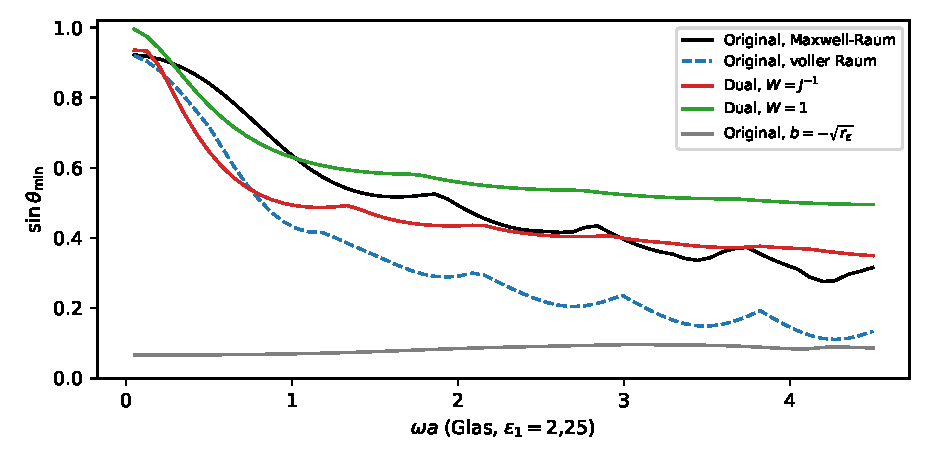
\includegraphics[width=0.92\textwidth]{fig_freq.pdf}
\caption{$\sin\theta_{\min}$ über der Frequenz für eine Glaskugel.}
\label{fig:freq}
\end{figure}

Klassische Formulierungen mit einem einzigen Randfeld versagen bei den
Dirichlet- oder Neumann-Eigenfrequenzen des Innengebiets. Abbildung~\ref{fig:freq}
zeigt über $\omega a\in[0{,}05;\,4{,}5]$ keinen Einbruch. Gezielte Auswertung an
allen Nullstellen von $j_l(k_ja)$ und $j_l'(k_ja)$ für $l\le2$, $j=1,2$
(13 Frequenzen, \texttt{candidates.py}) ergibt $\sin\theta_{\min}\ge 0{,}11$
(Original) bzw.\ $\ge0{,}35$ (dual). Die lokalen Minima der Kurven sind flach
($\sin\theta_{\min}$ nahe $\omega a = 4{,}27$ nach Minimierung $0{,}1105$). Sie sind
Mie-artige komplexe Resonanzen und keine reellen Singularitäten.

Die Wahl $b=-\sqrt{r_\varepsilon}$ liegt nach Satz~\ref{satz:symbol} auf der
Ausnahmemenge. Numerisch fällt $\sin\theta_{\min}$ dort bei Netzverfeinerung
monoton ($0{,}095$; $0{,}070$; $0{,}058$; $0{,}048$), während die Standardwahl bei
$0{,}4329$ bleibt. Das zeigt, dass das Symbolkriterium scharf ist. Die Wahl
$b=1$ statt $b=\sqrt{r_\varepsilon}$ ist praktisch gleichwertig.

\subsection{Permittivitätsstudie: eine echte Resonanz der Formulierung}

\begin{figure}[ht]
\centering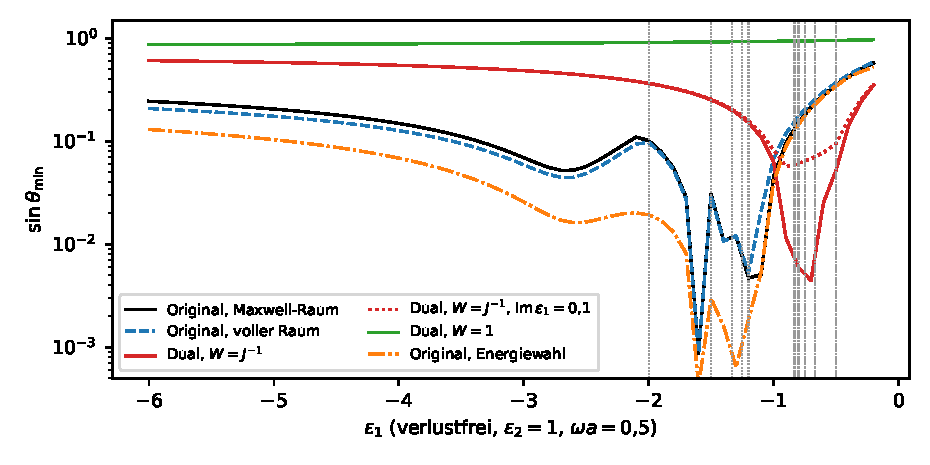
\includegraphics[width=0.92\textwidth]{fig_eps.pdf}
\caption{$\sin\theta_{\min}$ über reellem $\varepsilon_1<0$ bei $\omega a=0{,}5$.
Senkrechte Linien: quasistatische Kugelplasmonen $-(l+1)/l$ (punktiert) und
Hohlraumplasmonen $-l/(l+1)$ (strichpunktiert), $l=1,\dots,5$.}
\label{fig:eps}
\end{figure}

Abbildung~\ref{fig:eps} zeigt drei Befunde.
\begin{enumerate}[leftmargin=*]
  \item \emph{Originalproblem:} Maxwell- und voller Raum haben dieselben
    Einbrüche. Das sind die Oberflächenplasmonen der Kugel; die Dipolresonanz liegt
    retardierungsbedingt bei $\approx-2{,}7$ statt $-2$. Die Einbrüche höherer
    Ordnung sind tief, weil deren Strahlungsdämpfung wie $(\omega a)^{2l+1}$
    verschwindet. Die Hilfskomponenten erzeugen keine zusätzlichen Einbrüche.
  \item \emph{Duales Problem mit $W=J^{-1}$:} Es gibt einen scharfen Einbruch bei
    $\varepsilon_1^*\approx-0{,}6935$. Nach Minimierung ist
    $\sin\theta_{\min} = 3{,}3\cdot10^{-4}$ ($16\times32$) bzw.\ $6{,}4\cdot10^{-5}$
    ($20\times40$), also konvergent gegen null. Das duale Problem ist ein
    kugelförmiger Hohlraum in einem verlustfreien Metall. Dort ist
    $k_1 = \omega\sqrt{\varepsilon_1}$ rein imaginär, die Außenfelder klingen
    exponentiell ab, und es gibt keine Strahlungsdämpfung. Das Hohlraumplasmon ist
    deshalb ein echter reeller Eigenwert.
  \item Mit Verlust ($\operatorname{Im}\varepsilon_1 = 0{,}1$) bleibt der Einbruch
    endlich ($\sin\theta_{\min}\approx0{,}057$), bei geringem Verlust
    (z.\,B.\ Silber) aber entsprechend schlecht konditioniert.
\end{enumerate}

\begin{korollar}[Widerlegung von Vermutung \ref{verm:inj} für $W=J^{-1}$]\label{kor:widerlegt}
\status{numerisch belegt}
Für verlustfreie Metalle ($\varepsilon_1<0$ reell, $\omega>0$) ist das duale
Problem \eqref{eq:dual} nicht für alle $\varepsilon_1$ eindeutig lösbar. Die
Gleichung $T$ aus \eqref{eq:T} besitzt dann nichttriviale Kerne bei
$\varepsilon_1$-Werten, bei denen das physikalische Streuproblem eindeutig lösbar
ist. $T$ hat also \emph{falsche Resonanzen}. Sie liegen nahe den
Hohlraumplasmonen $-l/(l+1)\,\varepsilon_2$ der komplementären Geometrie.
\end{korollar}

\subsection{Resonanzfreie Formulierung}

Die Herleitung von \eqref{eq:T} lässt eine Freiheit: Die zweite Bedingung
$E_1^-Jh=0$ darf vor dem Addieren mit einem beliebigen invertierbaren $W$
multipliziert werden:
\begin{equation}\label{eq:TW}
  T_Wh := \big(E_2^+ + W E_1^-J\big)h = h^{\mathrm{inc}} .
\end{equation}

\begin{lemma}\label{lem:TW}\status{bewiesen}
Ist \eqref{eq:trans} eindeutig lösbar und gilt
$\operatorname{ran}E_2^+\cap W\operatorname{ran}E_1^- = \{0\}$, so ist $T_W$ injektiv,
und jede Lösung von \eqref{eq:TW} löst \eqref{eq:trans}.
\end{lemma}
\begin{proof}
Wörtlich wie Lemma~\ref{lem:Taequiv}, mit $W$ statt $J^{-1}$.
\end{proof}

Für $W=J^{-1}$ ist die duale Bedingung ein physikalisches Transmissionsproblem und
kann Eigenwerte haben (Korollar~\ref{kor:widerlegt}). Für $W=1$ verlangt sie
dagegen \emph{stetige Spur des vollen Multivektors} über $\Gamma$, ohne jede
Materialskalierung. Dafür gibt es eine Energieidentität.

\begin{lemma}[Flussidentität]\label{lem:fluss}\status{bewiesen, num.\ verif.}
Sei $A^\dagger := \tilde{A}^*$ und für ein Multivektorfeld $G$ das Vektorfeld
$\mvec{j}[G]$ mit Komponenten $j_l = \grade{G^\dagger\mvec{e}_lG}{0}$. Erfüllt $G$
die Gleichung $\nabla G = i\kappa G$ mit $\kappa\in\mathbb{C}$, so gilt
\[
  \nabla\cdot\mvec{j}[G] = -2\operatorname{Im}\kappa\,|G|^2,\qquad |G|^2 = \grade{G^\dagger G}{0}.
\]
\end{lemma}
\begin{proof}
$\nabla\cdot\mvec{j} = \sum_l\big(\grade{(\partial_lG)^\dagger\mvec{e}_lG}{0} +
\grade{G^\dagger\mvec{e}_l\partial_lG}{0}\big) = \grade{(\nabla G)^\dagger G}{0} +
\grade{G^\dagger\nabla G}{0}$, denn $(\mvec{e}_l\partial_lG)^\dagger =
(\partial_lG)^\dagger\mvec{e}_l$. Einsetzen von $\nabla G = i\kappa G$ gibt
$(-i\bar\kappa + i\kappa)|G|^2$. Numerische Prüfung für drei komplexe $\kappa$ in
\texttt{check\_flux.py}.
\end{proof}

\begin{satz}[Duale Bedingung für $W=1$]\label{satz:dualW1}\status{bewiesen, glatter Rand}
Seien $\operatorname{Im}k_1\ge0$, $\operatorname{Im}k_2\ge0$, $k_1\neq0$. Dann gilt
$\operatorname{ran}E_2^+\cap\operatorname{ran}E_1^-=\{0\}$ auf dem vollen Raum
$L^2(\Gamma;\clc)$, insbesondere auch für $\operatorname{Re}\varepsilon_1<0$ und
ohne Verlust.
\end{satz}
\begin{proof}
Sei $g$ im Schnitt: $g$ ist Spur einer inneren $k_2$-Lösung $G_i$ und einer
äußeren strahlenden $k_1$-Lösung $G_a$. Das zusammengesetzte Feld $G$ hat stetige
Spur, also ist $\n\cdot\mvec{j}[G]$ über $\Gamma$ stetig ($\mvec{j}$ hängt nur von
$G$ ab, nicht von $\varepsilon,\mu$). Integration von Lemma~\ref{lem:fluss} über
$B_R$ ergibt
\[
  \int_{S_R}\xh\cdot\mvec{j}\,dS = -2\operatorname{Im}k_2\!\int_\Omega|G|^2
  - 2\operatorname{Im}k_1\!\int_{B_R\setminus\Omega}|G|^2 .
\]
Aus der Strahlungsbedingung \eqref{eq:rad} folgt $\xh\cdot\mvec{j} =
\grade{G^\dagger\xh G}{0} = |G|^2 + o(r^{-2})$. Die linke Seite ist also
asymptotisch nichtnegativ und die rechte nichtpositiv, beide verschwinden. Ist
$\operatorname{Im}k_1>0$ (das schließt verlustfreie Metalle ein, da dort
$k_1\in i\mathbb{R}_+$), so ist $G_a\equiv0$. Ist $k_1$ reell, so folgt
$\int_{S_R}|G_a|^2\to0$, und nach dem Rellich-Lemma (komponentenweise, jede
Komponente ist eine strahlende Helmholtz-Lösung) ist $G_a\equiv0$. In beiden
Fällen ist $g=0$.
\end{proof}

\begin{korollar}[Resonanzfreiheit von $T_1$]\label{kor:T1}\status{bewiesen, glatter Rand}
Die Gleichung
\begin{equation}\label{eq:T1}
  T_1h = \big(E_2^+ + E_1^-J\big)h
  = \tfrac12(1+J)\,h + \tfrac12\big(\EG^{k_2}-\EG^{k_1}J\big)h = h^{\mathrm{inc}}
\end{equation}
ist für passive Medien genau dann eindeutig lösbar, wenn das physikalische
Transmissionsproblem \eqref{eq:trans} auf dem vollen Raum eindeutig lösbar ist.
Ihr Hauptsymbol hat
\[
  \det\sigma(T_1)\propto (r_\varepsilon+1)(r_\mu+1)(a+\sqrt{r_\mu})(b+\sqrt{r_\varepsilon}),
\]
dieselbe Ausnahmemenge wie Satz~\ref{satz:symbol} (nur einfach statt doppelt).
$T_1$ ist dann Fredholm vom Index~0.
\end{korollar}
\begin{proof}
Lemma~\ref{lem:TW} mit Satz~\ref{satz:dualW1} und Fredholm-Alternative. Die
Symbolrechnung ist Teil~8 des Skripts \texttt{symbol\_analysis.py}. Der Index folgt wie in
Satz~\ref{satz:symbol}, da $T_1=1$ für $J=1$.
\end{proof}

\begin{bemerkung}[Spektrum von $T_1$]\label{bem:T1spek}
Mit der Standardwahl hat $\sigma(T_1)$ die Eigenwerte $1$ (vierfach) sowie
\[
  \sqrt{r_\varepsilon},\quad \sqrt{r_\mu},\quad
  \tfrac12\big(\sqrt{r_\varepsilon}+1/\sqrt{r_\varepsilon}\big),\quad
  \tfrac12\big(\sqrt{r_\mu}+1/\sqrt{r_\mu}\big).
\]
Für jedes passive Medium mit $\operatorname{Im}\varepsilon_1>0$ liegt
$\sqrt{r_\varepsilon}$ im offenen ersten Quadranten, und alle Eigenwerte haben
positiven Realteil. Für dielektrische Kontraste sind sie reell und $\ge1$. Für Gold
($r_\varepsilon=-11+1{,}2i$) sind sie $0{,}18+3{,}32i$ und $0{,}10+1{,}51i$. Zum
Vergleich hatte $T$ (Bemerkung~\ref{bem:nichtkompakt}) dort ein indefinites
Spektrum $\{-0{,}81;\,2{,}81\}$. Die Multiplikation mit $2(1+J)^{-1}$ ist
punktweise und billig; sie bringt \eqref{eq:T1} auf die Form Identität plus
Operator nullter Ordnung.

Konsequenz für den Antrag: $T_1$ ersetzt $T$ als Standardformulierung in AP~1 und
AP~2. H1 sollte mit $T_1$ geprüft werden.
\end{bemerkung}

\subsection{Niederfrequenzverhalten auf der Kugel (Schritt 1.4, erster Teil)}

\begin{figure}[ht]
\centering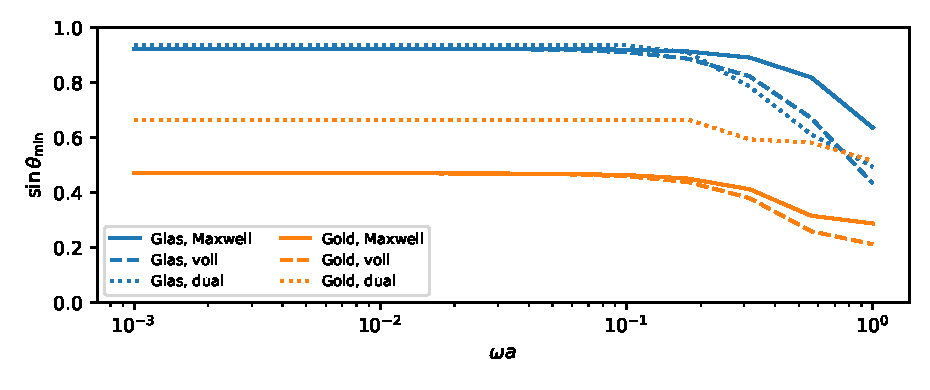
\includegraphics[width=0.92\textwidth]{fig_lowfreq.pdf}
\caption{$\sin\theta_{\min}$ für $\omega a\in[10^{-3};1]$ (Glas und Gold,
Original, voller Raum und dual mit $W=J^{-1}$).}
\label{fig:lowfreq}
\end{figure}

Für $\omega a\to0$ konvergieren alle Winkel gegen positive Grenzwerte
(Abbildung~\ref{fig:lowfreq}; bei $\omega a=10^{-3}$ z.\,B.\ Gold, voller Raum
$0{,}47$). Auf der einfach zusammenhängenden Kugel gibt es also keinen
Niederfrequenz-Zusammenbruch, weder in den physikalischen noch in den
Hilfsgraden. Das ist konsistent mit der Skalierung
$\mvec{F}=\sqrt\varepsilon\mvec{E}+I\sqrt\mu\mvec{H}$, die elektrische und
magnetische Anteile gleich gewichtet. Für Gebiete mit Henkeln (Torus,
Split-Ring) folgt der Test in Teil~III. Dort wurde zunächst ein
endlichdimensionaler Defekt der Dimension der ersten Betti-Zahl erwartet; Teil~III
(Abschnitt~\ref{sec:teil3}) zeigt, dass er nicht auftritt.

\subsection{Aktualisierter Stand zu Vermutung \ref{verm:inj}}

\begin{vermutung}\label{verm:inj2}\status{Vermutung, numerisch gestützt}
Für passive Medien und die Standardwahl $a=\sqrt{r_\mu}$, $b=\sqrt{r_\varepsilon}$
ist das Transmissionsproblem \eqref{eq:trans} auf dem vollen Raum
$L^2(\Gamma;\clc)$ eindeutig lösbar, außer bei $\varepsilon_1=-\varepsilon_2$ oder
$\mu_1=-\mu_2$. Mit Korollar~\ref{kor:T1} ist $T_1$ dann für alle passiven Medien
invertierbar.
\end{vermutung}

Stützend wirken: keine Einbrüche jenseits der physikalischen (Maxwell-)Resonanzen
in allen Studien, und Hilfskomponenten auf Residuumsniveau in der Streudemo. Der
fehlende Schritt ist eine Energieidentität für das Originalproblem. Die Rechnung
$\n\cdot\mvec{j}[\mvec{F}] = 2\operatorname{Re}\big(\sqrt{\varepsilon}\,
\overline{\sqrt{\mu}}\ \n\cdot(\mvec{E}\times\overline{\mvec{H}})\big)$ (für Grade 1,2)
zeigt, warum $\mvec{j}$ allein nicht reicht: Der Faktor
$\sqrt\varepsilon\,\overline{\sqrt\mu}$ springt über $\Gamma$. Nötig ist eine
gewichtete Variante, die auf den Graden 1,2 den Poynting-Fluss
$\operatorname{Re}(\mvec{E}\times\overline{\mvec{H}})$ und auf den Hilfsgraden
einen positiven Beitrag liefert.

%======================================================================
\section{Teil III: Eindeutigkeit im vollen Raum und Torus}\label{sec:teil3}
%======================================================================

\subsection{Zerlegung in Maxwell- und Hilfsanteil}

\begin{satz}[Maxwell-Hilfs-Zerlegung]\label{satz:zerlegung}\status{bewiesen, num.\ verif.}
Sei $k\neq0$ und $(\nabla-ik)G=0$ mit $G = \alpha + \mvec{a} + I\mvec{b} + I\beta$.
Dann ist $u := \alpha + I\beta$ eine (skalar-pseudoskalare) Helmholtz-Lösung, und
\[
  G = G_M + \tfrac{1}{ik}(\nabla+ik)\,u,
\]
wobei $G_M$ nur die Grade 1 und 2 hat und $(\nabla-ik)G_M=0$ erfüllt. $G_M$ ist also
ein Maxwell-Feld (Satz~\ref{satz:maxwell}). Die Zerlegung ist eindeutig, und
strahlendes $G$ hat strahlende Anteile.
\end{satz}
\begin{proof}
Nach Bemerkung~\ref{bem:hilfs} gilt $(\Delta+k^2)\alpha = (\Delta+k^2)\beta = 0$, also
$(\nabla-ik)(\nabla+ik)u = 0$. Der Hilfsterm ist deshalb selbst eine Dirac-Lösung,
und seine Grade 0 und 3 sind genau $u$. Somit hat $G_M$ keine Grade 0 und 3.
Eindeutigkeit: $u$ ist durch $\grade{G}{0}$ und $\grade{G}{3}$ festgelegt.
Numerische Prüfung: \texttt{check\_decomp.py}.
\end{proof}

Der Satz zeigt, dass die Hilfskomponenten nichts anderes sind als ein
angehängtes skalares Helmholtz-Problem. In der Transmissionsbedingung $h_1 =
Jh_2$ koppeln sie an die Maxwell-Anteile, weil $\frac{1}{ik}\nabla\alpha$ zum
Grad-1-Anteil beiträgt.

\subsection{Gewichteter Energiefluss}

Wir schreiben $G$ in den unskalierten Größen: $\mvec{E} := \grade{G}{1}/\sqrt\varepsilon$,
$\mvec{H} := -I\grade{G}{2}/\sqrt\mu$, $\alpha = \grade{G}{0}$, $I\beta = \grade{G}{3}$.
$\mvec{E},\mvec{H}$ enthalten dabei die Gradientenbeiträge der Hilfsanteile. Die
Gradzerlegung von $(\nabla-ik)G=0$ lautet dann
\begin{equation}\label{eq:maxaux}
  \nabla\times\mvec{E} = i\omega\mu\mvec{H} - \tfrac{1}{\sqrt\varepsilon}\nabla\beta,\quad
  \nabla\times\mvec{H} = -i\omega\varepsilon\mvec{E} + \tfrac{1}{\sqrt\mu}\nabla\alpha,\quad
  \nabla\cdot\mvec{E} = i\omega\sqrt\mu\,\alpha,\quad
  \nabla\cdot\mvec{H} = i\omega\sqrt\varepsilon\,\beta .
\end{equation}

\begin{lemma}[Energieidentität]\label{lem:energie}\status{bewiesen, num.\ verif.}
Für
\[
  \mvec{S} := \mvec{E}\times\overline{\mvec{H}}
  + \frac{\bar\alpha}{\overline{\sqrt\mu}}\,\mvec{E}
  + \frac{\beta}{\sqrt\varepsilon}\,\overline{\mvec{H}}
\]
gilt
\[
  \operatorname{Re}\nabla\cdot\mvec{S} = -\omega\Big[
  \operatorname{Im}\varepsilon\,|\mvec{E}|^2 + \operatorname{Im}\mu\,|\mvec{H}|^2
  + \sin(\arg\mu)\,|\alpha|^2 + \sin(\arg\varepsilon)\,|\beta|^2\Big] \le 0
\]
für jedes passive Medium, $\arg\varepsilon,\arg\mu\in[0,\pi]$, insbesondere für
Metalle mit $\operatorname{Re}\varepsilon<0$.
\end{lemma}
\begin{proof}
Mit \eqref{eq:maxaux} ist
$\nabla\cdot(\mvec{E}\times\overline{\mvec{H}}) = i\omega\mu|\mvec{H}|^2 - i\omega\bar\varepsilon|\mvec{E}|^2
- \overline{\mvec{H}}\cdot\nabla\beta/\sqrt\varepsilon - \mvec{E}\cdot\nabla\bar\alpha/\overline{\sqrt\mu}$.
Die beiden Gradiententerme heben sich gegen
$\nabla\cdot(\bar\alpha\mvec{E}) = \nabla\bar\alpha\cdot\mvec{E} + i\omega\sqrt\mu|\alpha|^2$
und $\nabla\cdot(\beta\overline{\mvec{H}}) = \nabla\beta\cdot\overline{\mvec{H}} -
i\omega\overline{\sqrt\varepsilon}|\beta|^2$ weg. Übrig bleibt
$\nabla\cdot\mvec{S} = i\omega\mu|\mvec{H}|^2 - i\omega\bar\varepsilon|\mvec{E}|^2 +
i\omega e^{2i\arg\sqrt\mu}|\alpha|^2 - i\omega e^{-2i\arg\sqrt\varepsilon}|\beta|^2$, und
$2\arg\sqrt\varepsilon = \arg\varepsilon$ (Hauptzweig). Numerische Prüfung für vier
Medien in \texttt{check\_energy.py}.
\end{proof}

\begin{lemma}[Stetigkeit des Flusses]\label{lem:flussJ}\status{bewiesen, num.\ verif.}
Sei $\sqrt{r_\varepsilon} := \sqrt{\varepsilon_1}/\sqrt{\varepsilon_2}$,
$\sqrt{r_\mu} := \sqrt{\mu_1}/\sqrt{\mu_2}$ (Wurzeln je Medium), und seien die
Hilfsparameter in $J$ durch die \emph{Energiewahl}
\begin{equation}\label{eq:energiewahl}
  a = \overline{r_\varepsilon}\,\sqrt{r_\mu},\qquad b = \overline{r_\mu}\,\sqrt{r_\varepsilon}
\end{equation}
festgelegt. Aus $h_1 = Jh_2$ folgt $\n\cdot\mvec{S}_1 = \n\cdot\mvec{S}_2$ auf $\Gamma$.
\end{lemma}
\begin{proof}
$J$ bewirkt $\mvec{E}_{1,T}=\mvec{E}_{2,T}$, $\mvec{H}_{1,T}=\mvec{H}_{2,T}$,
$\varepsilon_1E_{1,n} = \varepsilon_2E_{2,n}$ und $\mu_1H_{1,n}=\mu_2H_{2,n}$. Der
Term $\n\cdot(\mvec{E}\times\overline{\mvec{H}})$ hängt nur von Tangentialanteilen
ab. Für den zweiten Term gilt $\bar\alpha_1E_{1,n}/\overline{\sqrt{\mu_1}} =
\bar a\,(\varepsilon_2/\varepsilon_1)\,\bar\alpha_2E_{2,n}/\overline{\sqrt{\mu_1}}$,
und das ist genau dann $\bar\alpha_2E_{2,n}/\overline{\sqrt{\mu_2}}$, wenn $\bar a =
r_\varepsilon\overline{\sqrt{r_\mu}}$. Der dritte Term ist analog.
\end{proof}

Für reelle positive Kontraste ist \eqref{eq:energiewahl} $a = r_\varepsilon\sqrt{r_\mu}$,
$b=r_\mu\sqrt{r_\varepsilon}$. Im nichtmagnetischen Fall ($r_\mu=1$) stimmt $b$ mit der
Standardwahl überein, nur $a$ ändert sich von $1$ zu $\overline{r_\varepsilon}$. Die
Energiewahl liegt nie auf der Ausnahmemenge von Satz~\ref{satz:symbol}, denn
$a = -\sqrt{r_\mu}$ ist äquivalent zu $\overline{r_\varepsilon} = -1$.

\subsection{Eindeutigkeit und Invertierbarkeit}

\begin{satz}[Eindeutigkeit im vollen Raum]\label{satz:eind}\status{bewiesen, reguläre Lösungen}
Sei $\omega>0$, das Außenmedium verlustfrei ($\varepsilon_2,\mu_2>0$) und das
Innenmedium passiv (beliebiges $\operatorname{Re}\varepsilon_1$, auch verlustfrei).
Mit der Energiewahl \eqref{eq:energiewahl} hat das homogene Transmissionsproblem
\eqref{eq:trans} auf dem vollen Raum $L^2(\Gamma;\clc)$ nur die triviale Lösung.
\end{satz}
\begin{proof}
Sei $G_1$ innen, $G_2$ außen strahlend, $h_1 = Jh_2$. Mit
Lemma~\ref{lem:flussJ} und dem Gaußschen Satz auf $\Omega$ und $B_R\setminus\Omega$
heben sich die Beiträge auf $\Gamma$ weg:
\[
  \operatorname{Re}\int_{S_R}\xh\cdot\mvec{S}_2\,dS
  = \operatorname{Re}\int_\Omega\nabla\cdot\mvec{S}_1
  + \operatorname{Re}\int_{B_R\setminus\Omega}\nabla\cdot\mvec{S}_2 \le 0
\]
nach Lemma~\ref{lem:energie}. Nach Satz~\ref{satz:zerlegung} ist $G_2 = G_M +
\frac1{ik_2}(\nabla+ik_2)u$ mit strahlenden Anteilen. Asymptotisch trägt der
Hilfsteil $(1+\xh)u$ bei, also einen radialen Beitrag $\xh\alpha/\sqrt{\varepsilon_2}$
zu $\mvec{E}$ und $\xh\beta/\sqrt{\mu_2}$ zu $\mvec{H}$. Alle Kreuzterme mit den
transversalen Maxwell-Anteilen verschwinden in $\xh\cdot\mvec{S}$, und es bleibt
\[
  r^2\,\xh\cdot\mvec{S}_2 \to \sqrt{\varepsilon_2/\mu_2}\,|\mvec{E}_{M,\infty}|^2
  + \frac{|\alpha_\infty|^2 + |\beta_\infty|^2}{\sqrt{\varepsilon_2\mu_2}} \;\ge\; 0 .
\]
Also verschwinden alle Fernfeldmuster, und nach dem Rellich-Lemma (für Maxwell und
Helmholtz) ist $G_2\equiv0$. Dann ist $h_2 = 0$, $h_1 = Jh_2 = 0$, und nach
Satz~\ref{satz:cauchy-int} ist $G_1 = \mathcal{C}_{k_1}h_1 = 0$.
\end{proof}

\begin{korollar}[Invertierbarkeit von $T_1$]\label{kor:T1inv}\status{bewiesen, glatter Rand}
Unter den Voraussetzungen von Satz~\ref{satz:eind} und für glatten Rand ist $T_1$
mit der Energiewahl für alle passiven Innenmedien mit $\varepsilon_1\neq-\varepsilon_2$,
$\mu_1\neq-\mu_2$ ein Isomorphismus auf $L^2(\Gamma;\clc)$.
Vermutung~\ref{verm:inj2} ist damit für die Energiewahl bewiesen; für die
Standardwahl folgt sie aus Satz~\ref{satz:eindstd} (Teil V).
\end{korollar}
\begin{proof}
Injektivität aus Satz~\ref{satz:eind}, Lemma~\ref{lem:TW} und
Satz~\ref{satz:dualW1}. Fredholm vom Index~0 nach Korollar~\ref{kor:T1}.
\end{proof}

\subsection{Spektrum und Wahl der Hilfsparameter}

Für allgemeine $a,b$ hat $\sigma(T_1)$ die Eigenwerte $1$ (vierfach),
$\tfrac12(\sqrt{r_\varepsilon}+1/\sqrt{r_\varepsilon})$,
$\tfrac12(\sqrt{r_\mu}+1/\sqrt{r_\mu})$ sowie die beiden Hilfseigenwerte
$\tfrac12(a+\sqrt{r_\mu})$ und $\tfrac12(b+\sqrt{r_\varepsilon})$
(\texttt{symbol\_analysis.py}, Teil 10). Bei der Energiewahl ist
$\tfrac12(a+\sqrt{r_\mu}) = \tfrac12(\overline{r_\varepsilon}+1)\sqrt{r_\mu}$. Für
Metalle mit $\operatorname{Re}\varepsilon_1<-\varepsilon_2$ hat dieser Eigenwert
negativen Realteil, für Gold $-5{,}0-0{,}6i$. Die Vorkonditionierung mit der
punktweisen Multiplikation $2(1+J)^{-1}$ aus Bemerkung~\ref{bem:T1spek} behebt
das. Im nichtmagnetischen Fall sind die Symbolspektren von $2(1+J)^{-1}T_1$ für
Standard- und Energiewahl identisch (Teil 11), und alle Eigenwerte haben in den
getesteten Fällen positiven Realteil:

\begin{center}\small
\begin{tabular}{ll}
\toprule
$r_\varepsilon$ & nichttriviale Eigenwerte von $2(1+J)^{-1}\sigma(T_1)$\\
\midrule
$2{,}25$ & $0{,}80$; $1{,}00\pm0{,}20i$; $1{,}20$\\
$12$ & $0{,}45$; $1{,}00\pm0{,}55i$; $1{,}55$\\
$-11+1{,}2i$ & $0{,}19-0{,}54i$; $0{,}47+0{,}81i$; $1{,}54-0{,}81i$; $1{,}81+0{,}54i$\\
$-2+0{,}3i$ & $0{,}12+0{,}32i$; $0{,}68-0{,}88i$; $1{,}32+0{,}88i$; $1{,}88-0{,}32i$\\
\bottomrule
\end{tabular}
\end{center}

\emph{Empfehlung:} Energiewahl (beweisbar eindeutig) mit Vorkonditionierung
$2(1+J)^{-1}$ (günstiges Spektrum). Das ist die Formulierung, die in AP~2
diskretisiert werden sollte.

\subsection{Numerische Bestätigung auf der Kugel}

Die Streudemo mit Energiewahl (\texttt{scatter\_demo.py energy}) liefert dieselben
Ergebnisse wie mit der Standardwahl: Hilfsanteil $\le 9\cdot10^{-5}$, Abweichung
zum Maxwell-Raum $\le2\cdot10^{-6}$ und $Q_{\mathrm{ext}}$ gleich der Mie-Lösung
auf 4 bis 5 Stellen. In der Permittivitätsstudie (Abbildung~\ref{fig:eps},
strichpunktiert) liegen die Einbrüche wieder nur bei den physikalischen
Plasmonresonanzen. Sie sind etwas tiefer als mit der Standardwahl, weil die
Skalierung $a=\overline{r_\varepsilon}$ die $L^2$-Geometrie der Hilfsgrade verändert.
$\sin\theta_{\min}$ ist nicht invariant unter solchen Umskalierungen.

\subsection{Niederfrequenz auf dem Torus (Schritt 1.4, zweiter Teil)}

\paragraph{Methode.} Der Torus ($R=1$, $r=0{,}4$) ist rotationssymmetrisch um
$\mvec{e}_3$. Die zyklische Gruppe $C_n$ wirkt auf Spuren durch $h\mapsto
\mathcal{R}\,h(\mathcal{R}^{-1}\mvec{x})\,\tilde{\mathcal{R}}$ mit dem Rotor
$\mathcal{R} = e^{-\mvec{e}_{12}\pi/n}$. Dirac-Kern, Dipolfelder, Normale und $J$ sind
äquivariant. Mit Quellen auf $C_n$-Orbits und einem $C_n$-invarianten
Quadraturgitter ($n\cdot L$ Punkte in $\varphi$) zerfallen beide Spurräume
orthogonal in $n$ azimutale Moden. Die Hauptwinkel sind die Vereinigung der
Hauptwinkel je Mode (\texttt{torus\_sym.py}). Das reduziert den Aufwand um den
Faktor $n^2$. Der Abgleich mit der direkten Rechnung auf demselben Gitter ist
exakt (alle Stellen).

\paragraph{Konvergenz.} Mit nur $L=2$ Quadraturpunkten je Quellenabstand in
$\varphi$ entstehen durch Aliasing falsche kleine Winkel (z.\,B.\ $0{,}071$ statt
$0{,}822$ für Maxwell/Glas). Ab $L=3$ sind die Werte bei weiterer Verfeinerung
stabil:

\begin{center}\small
\begin{tabular}{lccccc}
\toprule
($n_\theta$, $L$, $n$, Quellen/Orbit) & voll/Glas & voll/Gold & Maxwell/Glas & Maxwell/Gold & dual $W{=}1$/Glas\\
\midrule
(40, 3, 32, 12) & 0,6797 & 0,1085 & 0,8223 & 0,1354 & 0,6704\\
(48, 3, 40, 16) & 0,6797 & 0,1083 & 0,8220 & 0,1278 & 0,6704\\
(64, 4, 48, 20) & 0,6797 & 0,1083 & 0,8220 & 0,1275 & 0,6704\\
\bottomrule
\end{tabular}\\[2pt]
{\footnotesize $\omega R = 0{,}5$; Glas $\varepsilon_1 = 2{,}25$, Gold $\varepsilon_1 = -11+1{,}2i$.}
\end{center}

\begin{figure}[ht]
\centering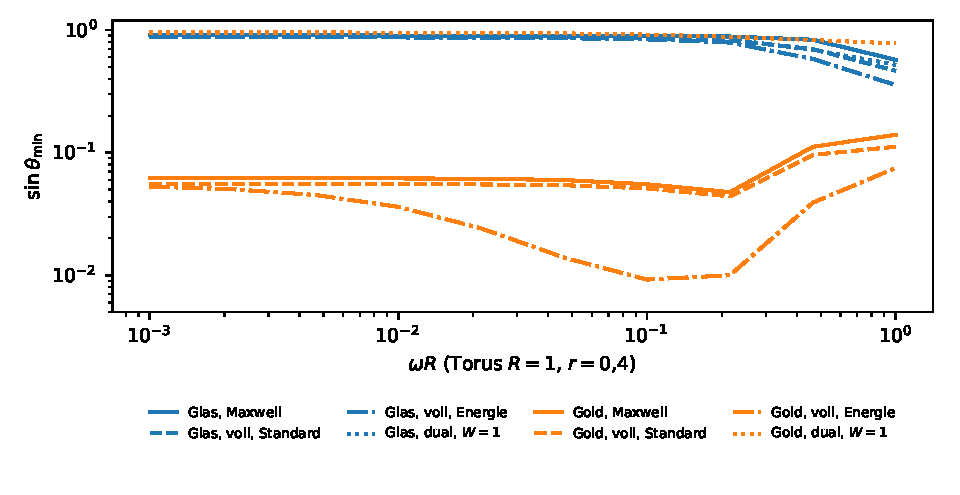
\includegraphics[width=0.92\textwidth]{fig_torus.pdf}
\caption{$\sin\theta_{\min}$ auf dem Torus für $\omega R\in[10^{-3};1]$.}
\label{fig:torus}
\end{figure}

\paragraph{Ergebnis.} Alle Winkel konvergieren für $\omega\to0$ gegen positive
Grenzwerte (Abbildung~\ref{fig:torus}, Gitter (48, 3, 40, 16)):
\begin{itemize}[leftmargin=*]
  \item Glas: $0{,}87$ (Standardwahl), $0{,}91$ (Maxwell), $0{,}95$ (dual, $W=1$).
  \item Gold: $0{,}055$ (Standardwahl), $0{,}062$ (Maxwell), $0{,}95$ (dual). Der kleinere
    Wert bei Gold ist physikalisch: Er tritt im Maxwell-Raum genauso auf, und zwar
    in den Moden $m=\pm1$. Das deutet auf eine nahe Dipolplasmonresonanz des Torus
    hin.
  \item Mit Energiewahl sinkt der Wert bei Gold um $\omega R\approx0{,}1$ auf
    $0{,}009$, erholt sich aber für $\omega\to0$ wieder auf $0{,}053$.
    Das ist ein Effekt der Metrik (siehe oben), keine Singularität.
\end{itemize}
Die in Teil~II erwartete endlichdimensionale Entartung über die Betti-Zahl tritt
\emph{nicht} auf. Der Grund ist, dass das Problem hier für die vollen Spuren
einschließlich der Normalkomponenten gestellt ist. Die im statischen Grenzfall
vorhandenen harmonischen Felder des Torus sind durch die Normalbedingungen
($\varepsilon E_n$, $\mu H_n$ stetig) eindeutig festgelegt, anders als in
Formulierungen, die nur Tangentialströme als Unbekannte verwenden
(Loop-Star-Problematik der EFIE). Der Niederfrequenz-Zusammenbruch klassischer
Verfahren ist eine Eigenschaft der Formulierung, nicht des Problems, und $T_1$
erbt ihn nach diesen Ergebnissen nicht. Ein Nachweis für die diskretisierte
Gleichung (AP~2) steht noch aus.

\subsection{Unabhängige Kontrolle: kontinuierliche Modenzerlegung}\label{sec:bor}

\paragraph{Methode.} Die Rechnung oben benutzt die diskrete Gruppe $C_n$.
Unabhängig davon wurde der Torus mit einer Zerlegung nach der
\emph{kontinuierlichen} Drehgruppe gerechnet (\texttt{bor.py}). Für jede Quelle
$\mvec{x}_s$ auf dem Meridian $\varphi=0$ und jeden Azimutalmodus $m$ ist
\[
  B_m(\mvec{x}) = \frac{1}{N_{\mathrm{rot}}}\sum_{j=1}^{N_{\mathrm{rot}}}
  e^{-im\varphi_j}\,\mathcal{R}_j\,F\big(\mathcal{R}_j^{-1}\mvec{x}\big)\,\tilde{\mathcal{R}}_j,
  \qquad \varphi_j = 2\pi j/N_{\mathrm{rot}},
\]
eine exakte Dirac-Lösung, die bis auf Aliasing der Ordnung $m\pm N_{\mathrm{rot}}$ im
Modus $m$ liegt. Ein solches Feld ist durch seine Werte auf dem Meridian bestimmt.
Die $L^2(\Gamma)$-Norm ist $2\pi\int|B_m|^2\rho\,d\ell$, und verschiedene Moden sind
orthogonal. Damit gilt exakt
\[
  \sin\theta_{\min} = \inf_{m\in\mathbb{Z}}\ \sin\theta_{\min}(m).
\]
Jeder Block hat nur $8\,n_q$ Zeilen ($n_q$ Meridianpunkte). Das erlaubt eine
Konvergenzstudie in allen Parametern.

\paragraph{Validierung.} Auf der Kugel reproduziert die Methode die 3D-Werte aus
Teil~II auf 5 Stellen ($0{,}63584$; $0{,}43293$; $0{,}19281$). Für wachsendes $m$
steigen die Kugelwerte gegen den Symbolwinkel an (Glas: $0{,}915$ bei
$m=5$, $0{,}928$ bei $m=10$, Symbol $0{,}933$). Die Werte aus Teil~II sind also
tatsächlich die globalen Minima. Auf dem Torus stimmt die Methode bei $\omega R=0{,}5$
mit der $C_n$-Rechnung oben überein: Gold, voller Raum $0{,}1083$, Maxwell $0{,}1275$.

\paragraph{Aliasing in Umfangsrichtung.} Die Drehquadratur ist die kritische
Stelle. Für den Torus (Quellenabstand zur Oberfläche $0{,}2$) ergibt sich im Modus
$m=0$ bei Glas, $\omega=1$:
\begin{center}\small
\begin{tabular}{lcccc}
\toprule
$N_{\mathrm{rot}}$ & 64 & 128 & 256 & 512\\
\midrule
Maxwell-Raum & 0,0202 & 0,5427 & 0,5704 & 0,5704\\
voller Raum & 0,0024 & 0,4668 & 0,4668 & 0,4668\\
dual, $W=1$ & 0,0029 & 0,5202 & 0,5202 & 0,5202\\
\bottomrule
\end{tabular}
\end{center}
Bei zu grober Quadratur entstehen \emph{scheinbare} Nullen, auch für das duale
Problem mit $W=1$, das nach Satz~\ref{satz:dualW1} beweisbar eindeutig lösbar ist.
Ursache ist das Zusammenspiel von Aliasing mit der Orthonormalisierung schlecht
konditionierter MFS-Basen: Richtungen mit kleinen Singulärwerten verstärken den
Aliasfehler. Dasselbe betrifft eine direkte 3D-Rechnung mit wenigen Quellen in
Umfangsrichtung. Frühere, nicht in dieses Dokument übernommene 3D-Torus-Werte
waren aus diesem Grund unzuverlässig. Alle folgenden Werte benutzen
$N_{\mathrm{rot}}=256$, $n_q=96$ und 24 Quellen je Meridian. Eine Verfeinerung auf
$(384,128,32)$ ändert keine der vier angegebenen Stellen, getestet für
$m\in\{0,1,2,4,8,12,16,-3\}$.

\paragraph{Grenzwert hoher Moden.} Für $|m|\to\infty$ konvergiert
$\sin\theta_{\min}(m)$ gegen den Winkel der Hauptsymbole. Das ist der Winkel
zwischen $J^{-1}\operatorname{ran}\tfrac12(1+\sigma)$ und
$\operatorname{ran}\tfrac12(1-\sigma)$ in $\mathbb{C}^8$, berechnet mit
\texttt{symbol\_angle.py}:
\begin{center}\small
\begin{tabular}{lcccccc}
\toprule
$r_\varepsilon$ & $1$ & $2{,}25$ & $12$ & $-11+1{,}2i$ & $-2+0{,}3i$ & $-1+0{,}1i$\\
\midrule
Symbolwinkel (Standardwahl) & 1 & 0,933 & 0,763 & 0,641 & 0,327 & 0,050\\
Symbolwinkel dual, $W=1$ & 1 & 1 & 1 & 1 & 1 & 1\\
\bottomrule
\end{tabular}
\end{center}
Der Symbolwinkel ist eine obere Schranke für $\sin\theta_{\min}$, und er hängt
nur vom Kontrast ab, nicht von der Geometrie. Bei $\varepsilon_1\to-\varepsilon_2$ geht er
gegen null; das ist die Ausnahmemenge aus Satz~\ref{satz:symbol}. Auf dem Torus ist
$\sin\theta_{\min}(16)$ für Glas $0{,}930$ und für Gold $0{,}596$, jeweils nahe am
Symbolwert.

\paragraph{Niederfrequenz.} Abbildung~\ref{fig:torus_lf} zeigt $\min_m
\sin\theta_{\min}(m)$ für $\omega\in\{0;10^{-6};\dots;1\}$. Die Werte für
$\omega\to0$ lauten Glas $0{,}872$ (voll, $m=1$), $0{,}898$ (Maxwell, $m=0$) und
$0{,}954$ (dual, $W=1$) sowie Gold $0{,}055$ (voll und Maxwell, jeweils $m=1$) und
$0{,}954$ (dual). Das bestätigt die Ergebnisse oben.

\begin{figure}[ht]
\centering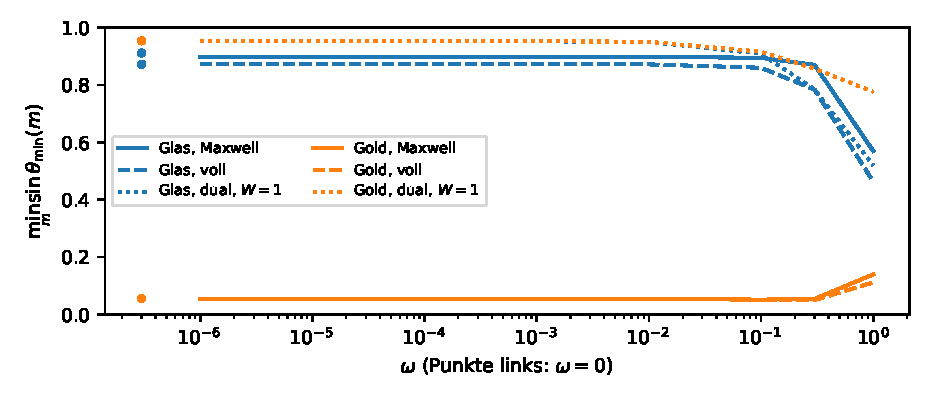
\includegraphics[width=0.92\textwidth]{fig_torus_lf.pdf}
\caption{Torus mit Modenzerlegung, $\min_m\sin\theta_{\min}(m)$ über $\omega$. Die
Punkte links sind die Werte bei exakt $\omega=0$.}
\label{fig:torus_lf}
\end{figure}

\begin{bemerkung}[Topologischer Fingerabdruck im Modus $m=0$]\label{bem:m0}
\status{numerische Beobachtung}
Im Maxwell-Raum ist $\sin\theta_{\min}(0)$ für alle $\omega\in[10^{-6},10^{-2}]$
gleich $0{,}8983$ (Glas), bei exakt $\omega=0$ aber $0{,}9252$. Für Gold ist es
$0{,}5979$ gegenüber $0{,}6067$. Alle anderen Moden sind stetig in $\omega=0$, und
auf der Kugel ist auch $m=0$ stetig. Der Grenzwert $\omega\to0$ des Maxwell-Problems
auf dem Torus stimmt also im Modus $m=0$ nicht mit dem statischen Problem überein.
$m=0$ ist genau der Sektor, der die harmonischen Felder des Torus enthält (Betti-Zahl
$b_1=1$). Eine plausible Erklärung: Ringe azimutal orientierter Dipole haben für
$\omega>0$ ein Feld der Ordnung $\mathcal{O}(k)$, das bei $\omega=0$ identisch
verschwindet. Die normierten Grenzfelder liegen deshalb nicht im statischen
Lösungsraum. Für die Stabilität ist das unerheblich, denn für $\omega>0$ bleibt der
Wert gleichmäßig beschränkt. Für eine Niederfrequenz-\emph{Asymptotik} (etwa
quasistatische Entwicklungen in AP~4) ist der Punkt aber zu beachten. Im vollen
Raum tritt der Sprung nicht auf.
\end{bemerkung}

\paragraph{Permittivitätsstudie auf dem Torus (verlustfrei, quasistatisch).}
Abbildung~\ref{fig:torus_eps} zeigt $\min_m\sin\theta_{\min}(m)$ für 24 reelle Werte
$\varepsilon_1\in[-30;-0{,}3]$ bei $\omega=10^{-3}$. Befunde:
\begin{enumerate}[leftmargin=*]
  \item \emph{Originalproblem:} Maxwell- und voller Raum stimmen an allen
    Stützstellen auf höchstens 3{,}7\,\% überein (größte Abweichung bei
    $\varepsilon_1=-0{,}7$: $0{,}0066$ gegenüber $0{,}0063$). Die Einbrüche sind Torus-Plasmonen: Modus $m=1$ nahe
    $-10$, $m=2$ nahe $-4$, $m=3$ nahe $-2{,}7$, höhere Moden gegen $-1$. Die
    Hilfsgrade erzeugen keine zusätzlichen Einbrüche, jedenfalls keine, die breiter
    als das Stützstellenraster sind.
  \item \emph{Dual mit $W=1$:} konstant $0{,}954$, in Übereinstimmung mit
    Satz~\ref{satz:dualW1}.
  \item \emph{Dual mit $W=J^{-1}$:} Einbrüche bis $2\cdot10^{-4}$ für
    $\varepsilon_1\in[-1{,}5;-0{,}3]$, dort, wo die Hohlraumplasmonen des
    komplementären Gebiets liegen. Das bestätigt Korollar~\ref{kor:widerlegt} auch
    auf dem Torus.
\end{enumerate}

\begin{figure}[ht]
\centering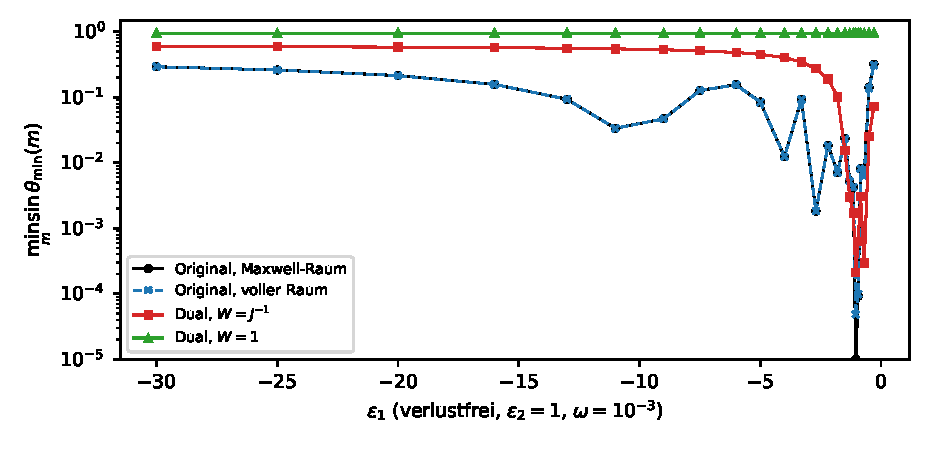
\includegraphics[width=0.92\textwidth]{fig_torus_eps.pdf}
\caption{Torus, verlustfrei, $\omega=10^{-3}$: $\min_m\sin\theta_{\min}(m)$ über
$\varepsilon_1$ für Original- und duales Problem.}
\label{fig:torus_eps}
\end{figure}

\paragraph{Energie- und Standardwahl auf dem Torus.} Zum Vergleich
(alle Moden $m\in\{0,\dots,6,16\}$):
\begin{center}\small
\begin{tabular}{lccc}
\toprule
Fall & Energiewahl & Standardwahl & Maxwell-Raum\\
\midrule
Glas, $\omega=1$ & 0,356 & 0,464 & 0,570\\
$\varepsilon_1=-9$, $\omega=10^{-3}$ & 0,045 & 0,047 & 0,047\\
$\varepsilon_1=-4$, $\omega=10^{-3}$ & 0,012 & 0,012 & 0,012\\
$\varepsilon_1=-0{,}7$, $\omega=10^{-3}$ & 0,006 & 0,006 & 0,007\\
Gold, $\omega=0{,}5$ & 0,047 & 0,108 & 0,128\\
\bottomrule
\end{tabular}
\end{center}
Beide Wahlen folgen den physikalischen Resonanzen. Die kleineren Werte der
Energiewahl bei Glas und Gold sind der Metrikeffekt aus der Kugelstudie:
$a=\overline{r_\varepsilon}$ skaliert die Hilfsgrade in $L^2$ um. Sie sind keine
Aussage über die Kondition des vorkonditionierten Operators
$2(1+J)^{-1}T_1$, dessen Symbolspektrum für beide Wahlen gleich ist. Welche Wahl in
der Diskretisierung besser konditioniert ist, muss in AP~2 an den Systemmatrizen
selbst gemessen werden. \emph{Nachtrag:} Da Satz~\ref{satz:eindstd} die Eindeutigkeit auch für die
Standardwahl liefert und die Energiewahl an Kanten ungeeignet ist
(Korollar~\ref{kor:faktor}), wird die Standardwahl empfohlen.


%======================================================================
\section{Teil IV: Kanten (Schritt 1.5)}\label{sec:teil4}
%======================================================================

\subsection{Lokales Modell und Konormalsymbol}

An einer Kante mit Öffnungswinkel $\alpha$ des Gebiets $\Omega$ (Medium 1) ist
$\Gamma$ lokal das Produkt eines Winkels mit der Kantenrichtung $\mvec{e}_3$. Die
Fredholm-Eigenschaft in $L^2(\Gamma)$ verlangt neben dem Hauptsymbol
(Satz~\ref{satz:symbol}) die Invertierbarkeit des \emph{Konormalsymbols}, also des
Mellin-Symbols im Abstand $r$ zur Kante. Für $r\to0$ ist das Produkt
$r\,\xi_3$ vernachlässigbar, und die Integration des 3D-Kerns über die
Kantenrichtung ergibt
\[
  \int_{\mathbb{R}}\frac{\mvec{z}_\perp + z_3\mvec{e}_3}{4\pi(|\mvec{z}_\perp|^2+z_3^2)^{3/2}}\,dz_3
  = \frac{\mvec{z}_\perp}{2\pi|\mvec{z}_\perp|^2},
\]
den 2D-Cauchy-Kern ($\mvec{e}_3$-Anteil ungerade). Das Konormalsymbol der Kante
ist deshalb das des Cauchy-Operators an einer 2D-Ecke, angewendet auf
$\clc$-wertige Dichten {\small\sffamily[Standard, Kantenkalkül; Skizze]}. Wir rechnen im
quasistatischen Grenzfall, der das Konormalsymbol bestimmt, und nichtmagnetisch
($\mu_1=\mu_2$).

\paragraph{Mellin-Symbol.} Der Rand bestehe aus zwei Strahlen $t\mvec{d}_j$
($t>0$) mit äußeren Normalen $\n_j$. Für Dichten $h_j(t) = t^{a-1}c_j$ mit
$c_j\in\mathbb{C}^8$ gilt $(\EG h)_i(s) = s^{a-1}\sum_j M_{ij}(a)c_j$ mit
\[
  M_{ii}(a) = -\cot(\pi a)\,\mvec{d}_i\n_i,\qquad
  M_{ij}(a) = -2\int_0^\infty\frac{\mvec{d}_i - u\mvec{d}_j}{2\pi|\mvec{d}_i-u\mvec{d}_j|^2}\,
  \n_j\,u^{a-1}\,du\quad(i\neq j),
\]
als Linksmultiplikation auf $\mathbb{C}^8$. Die Diagonale folgt aus
$\mathrm{p.v.}\int_0^\infty u^{a-1}(1-u)^{-1}du = \pi\cot(\pi a)$. Die $L^2$-Theorie
gehört zur Geraden $\operatorname{Re}a = \tfrac12$. Gewichtete Räume
$L^2(\Gamma, r^{2\beta}d\sigma)$ gehören zu $\operatorname{Re}a = \tfrac12-\beta$
(\texttt{corner.py}). Kontrolle: Wegen $\EG^2=1$ auf Lipschitz-Kurven muss
$M(a)^2 = 1$ gelten. Numerisch ist $\max|M^2-1|\le1{,}9\cdot10^{-12}$ für
$\alpha\in\{\pi/3,\pi/2,\pi,3\pi/2\}$ und mehrere $\tau$.

\subsection{Kritische Kontraste}

\begin{satz}[Konormalsymbol von $T_1$ an einer Ecke]\label{satz:ecke}
\status{geschlossene Form; Beweis über Satz~\ref{satz:faktor}}
Sei $\kappa = \varepsilon_1/\varepsilon_2$, $\mu_1=\mu_2$. Das Mellin-Symbol
$\sigma_M(T_1)(a) = \tfrac12(1+M(a)) + \tfrac12(1-M(a))J$ auf der Geraden
$\operatorname{Re}a=c$ ist genau dann singulär, wenn
\begin{equation}\label{eq:eckkrit}
  \frac{1+\kappa}{1-\kappa} = \pm S(a),\qquad
  S(a) = \frac{\sin((\pi-\alpha)a)}{\sin(\pi a)},\qquad a = c+i\tau,\ \tau\in\mathbb{R}.
\end{equation}
Die kritische Menge
$\mathcal{K}_c(\alpha) = \{\kappa = (\pm S(c+i\tau)-1)/(\pm S(c+i\tau)+1)\}$ ist
unabhängig von der Wahl der Hilfsparameter (getestet: Standard- und Energiewahl).
Sie stimmt exakt mit der kritischen Menge des skalaren quasistatischen
Transmissionsproblems überein, also mit
$-(\kappa+1)/(2(\kappa-1))\in\operatorname{spec}$ des Mellin-Symbols des
Neumann-Poincaré-Operators $K^*$.
\end{satz}

\noindent\emph{Nachweis.} Die kritischen $\kappa$ des $16\times16$-Symbols ergeben
sich als Eigenwerte eines quadratischen Eigenwertproblems in $\sqrt\kappa$
(\texttt{corner\_crit.py}). Sie stimmen mit \eqref{eq:eckkrit} auf
$10^{-8}$ bis $10^{-12}$ überein, für $\alpha\in\{\pi/3,\,1{,}3,\,\pi/2\}$,
$c\in\{0{,}5;\,0{,}3\}$ und $\tau\in\{0;\,0{,}4;\,1{,}5\}$. Die Gegenrechnung mit dem
unabhängig aufgestellten $2\times2$-Mellin-Symbol von $K^*$ stimmt auf allen
angegebenen Stellen (\texttt{corner\_np.py}). Für die Energiewahl ist der kleinste
Singulärwert auf der Kurve $7\cdot10^{-6}$, gleich dem der Standardwahl. Den
analytischen Hintergrund liefert die Blockfaktorisierung in
Abschnitt~\ref{sec:faktor}. Für $c=0{,}1$ ist die
Mellin-Quadratur nicht mehr genau genug (Abweichung bis $10^{-1}$); dort wird nur die
geschlossene Form verwendet.

\paragraph{Folgerungen aus der geschlossenen Form.}
\begin{itemize}[leftmargin=*]
  \item Für $\tau=0$ und $c=\tfrac12$ ist $S = \cos(\alpha/2)$. Die reellen Endpunkte
    sind $\kappa = -\cot^2(\alpha/4)$ und $-\tan^2(\alpha/4)$. Für die rechtwinklige
    Kante ($\alpha=\pi/2$ oder $3\pi/2$) sind das $-(1+\sqrt2)^2\approx-5{,}83$ und
    $-(\sqrt2-1)^2\approx-0{,}17$.
  \item Für $\tau\to\pm\infty$ geht $S\to0$ und $\kappa\to-1$: Die Kurven schließen
    sich im Punkt der glatten Ausnahmemenge.
  \item Für $c\to0$ wird $S(i\tau) = \sinh((\pi-\alpha)\tau)/\sinh(\pi\tau)$ reell.
    Die kritische Menge schrumpft auf das reelle Intervall
    $[-(2\pi-\alpha)/\alpha,\,-\alpha/(2\pi-\alpha)]$, für $\alpha=\pi/2$ also
    $[-3,-\tfrac13]$. Das ist das bekannte Intervall der Energie-Theorie
    (T-Koerzivität), eine unabhängige Plausibilitätskontrolle.
  \item Für $c=\tfrac12$ ($L^2$) ist $\mathcal{K}_{1/2}$ dagegen ein Paar
    \emph{komplexer} Schleifen. Die große reicht bei $\alpha=\pi/2$ bis
    $\operatorname{Im}\kappa\approx2{,}1$ (Abbildung~\ref{fig:corner}).
\end{itemize}

\begin{figure}[ht]
\centering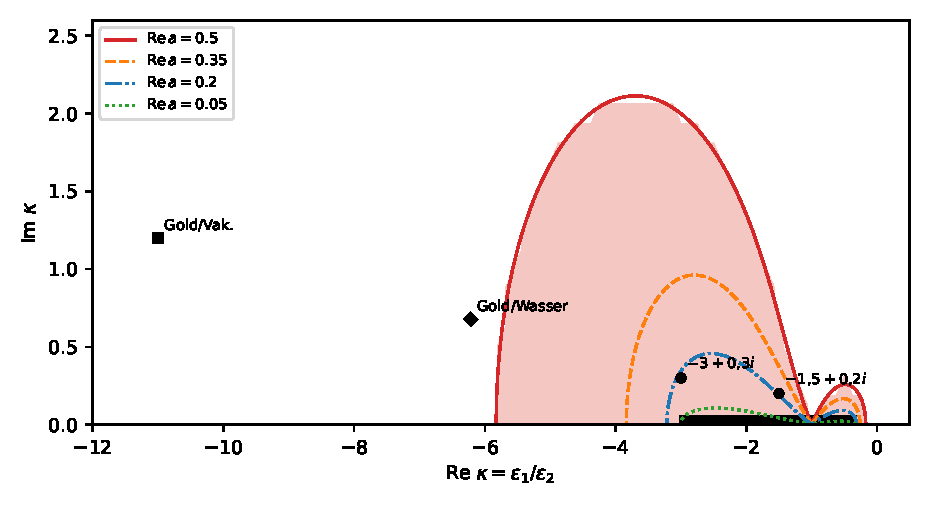
\includegraphics[width=0.92\textwidth]{fig_corner.pdf}
\caption{Kritische Mengen $\mathcal{K}_c(\pi/2)$ in der oberen Halbebene (passive
Medien) für verschiedene Mellin-Geraden. Schattiert ist das Gebiet mit
Windungszahl $+1$ für $L^2$ (Standardwahl). Schwarzer Balken: Intervall
$[-3,-\tfrac13]$ der Energie-Theorie.}
\label{fig:corner}
\end{figure}

\subsection{Index und physikalische Deutung}

Die Windungszahl von $\tau\mapsto\det\sigma_M(T_1)(\tfrac12+i\tau)$ ist innerhalb
der Schleifen $+1$ und außerhalb $0$ (Standardwahl, $\kappa$-Gitter mit
$69\times49$ Punkten, \texttt{corner\_index.py}). Die Kurve schließt sich jeweils
bis auf $10^{-11}$. Nach dem Indexsatz für Mellin-Operatoren ist $T_1$ innerhalb
der Schleifen Fredholm mit Index $\neq0$ {\small\sffamily[Standard]}, also nicht
invertierbar auf $L^2(\Gamma)$.

Physikalisch bedeutet das: Innerhalb der Schleifen besitzt das Kantenproblem einen
Singulärexponenten, für den die Randspur des Feldes wie $r^{a-1}$ mit
$\operatorname{Re}a<\tfrac12$ divergiert. Die physikalische Lösung existiert im
Energieraum (für $\operatorname{Im}\kappa>0$), ihre Spur liegt aber nicht in
$L^2$. Eine $L^2$-Formulierung kann sie deshalb nicht darstellen.

\begin{bemerkung}[Energiewahl; aufgeklärt in Abschnitt~\ref{sec:faktor}]\label{bem:eckenergie}
Mit der Energiewahl ($a=\bar\kappa$) ist die Windungszahl auch innerhalb der
Schleifen $0$. Die Singularitätskurve ist aber dieselbe. Die Hilfsgrade tragen
offenbar eine kompensierende Windung $-1$ bei. Da die physikalische Lösung nicht in
$L^2$ liegt, kann eine $L^2$-Lösung von $T_1$ dort nicht die physikalische sein.
$T_1$ ist dann entweder nicht injektiv, oder seine Lösung enthält Hilfsanteile
$\neq0$ {\small\sffamily[Folgerung, Skizze]}. Der Eindeutigkeitsbeweis
(Satz~\ref{satz:eind}) überträgt sich also nicht ohne Weiteres auf Ränder mit
Kanten.
\end{bemerkung}

\paragraph{Einordnung typischer Kontraste} (Werte für $\varepsilon$ nur
Größenordnung, zu prüfen):
\begin{center}\small
\begin{tabular}{lccc}
\toprule
Fall & $\kappa$ & Windung ($L^2$) & nötiges $\beta$ für $L^2(r^{2\beta})$\\
\midrule
Gold in Vakuum & $-11+1{,}2i$ & 0 & 0\\
Silber in Vakuum & $-15+0{,}5i$ & 0 & 0\\
Gold in Wasser & $-6{,}2+0{,}68i$ & 0 (knapp) & 0\\
$\kappa=-5+0{,}5i$ & & 1 & $\ge0{,}04$\\
$\kappa=-3+0{,}3i$ & & 1 & $\ge0{,}32$\\
$\kappa=-2+0{,}3i$ & & 1 & $\ge0{,}34$\\
$\kappa=-1{,}5+0{,}2i$ & & 1 & $\ge0{,}29$\\
$\kappa=-0{,}5+0{,}1i$ & & 1 & $\ge0{,}28$\\
\bottomrule
\end{tabular}\\[2pt]
{\footnotesize $\beta = \tfrac12-c^*$ mit dem größten $c^*$, für das $\kappa\notin$
Innengebiet von $\mathcal{K}_{c^*}$ (\texttt{corner\_weights.py}).
Für Gold in Wasser ist $\min_\tau|\det|/\max_\tau|\det| = 0{,}054$.}
\end{center}

\subsection{Konsequenzen für den Antrag}

\begin{enumerate}[leftmargin=*]
  \item \emph{H1 ist an Kanten in $L^2$ nicht haltbar,} und zwar genau im
    plasmonischen Resonanzbereich ($\operatorname{Re}\kappa\in(-5{,}8;-0{,}17)$ bei
    mäßigem Verlust für rechtwinklige Kanten). In diesem Bereich liegen
    typischerweise die quasistatischen Resonanzen von Nanowürfeln und -stäbchen
    (konkrete Werte zu prüfen). Außerhalb (Gold und Silber in Vakuum bei den obigen
    Werten) ist die $L^2$-Theorie an Kanten intakt.
  \item \emph{Prüfbare Vorhersage für AP~4:} Eine $L^2$-konforme Diskretisierung
    von $T_1$ auf dem Nanowürfel zeigt für $\kappa$ innerhalb der Schleifen bei
    Netzverfeinerung wachsende Iterationszahlen oder Stagnation, außerhalb nicht.
    Die Grenze ist die Kurve $\mathcal{K}_{1/2}(\pi/2)$.
  \item \emph{Abhilfe:} gewichtete Räume $L^2(r^{2\beta})$ mit
    $\beta>\tfrac12-\min_j\operatorname{Re}a_j$, typischerweise $\beta\approx0{,}35$ im
    Resonanzbereich (Abschnitt~\ref{sec:exponenten}). Im 2D-Prototyp
    realisiert Kollokation auf geometrisch gradierten Netzen dieses Gewicht
    (Abschnitt~\ref{sec:geo}). GMRES-Iterationen wachsen im plasmonischen Regime
    aber auch dann noch mit der Eckauflösung; eine eckangepasste
    Vorkonditionierung gehört deshalb in AP~2 und AP~3. Das ist eine Änderung an P2 und
    AP~2.
    Für verlustfreie $\kappa\in[-3,-\tfrac13]$ hilft kein Gewicht; das ist die
    physikalische Schlechtgestelltheit, die auch klassische Verfahren betrifft.
\end{enumerate}

\subsection{Singulärexponenten und nötige Gewichte}\label{sec:exponenten}

Die Nullstellen $a_j(\kappa)$ von $S(a)^2 - q^2$ mit $q=(1+\kappa)/(1-\kappa)$ im
Streifen $0<\operatorname{Re}a<1$ sind die Singulärexponenten der Kante. Die
Randspur verhält sich wie $r^{a_j-1}$ und liegt in $L^2(r^{2\beta})$ genau dann,
wenn $\operatorname{Re}a_j > \tfrac12-\beta$.

\begin{prop}\label{prop:cstar}\status{numerisch verifiziert}
Das größte $c^*\le\tfrac12$, für das $\kappa$ außerhalb des Innengebiets von
$\mathcal{K}_{c^*}(\alpha)$ liegt, ist $c^* = \min(\tfrac12,\ \min_j\operatorname{Re}a_j(\kappa))$.
Das nötige Gewicht ist also $\beta \ge \tfrac12 - \min_j\operatorname{Re}a_j$.
\end{prop}

Für $\alpha=\pi/2$ (\texttt{exponents.py}; Nullstellensuche im Streifen gegen die
Windungsgrenze $c^*$ aus \texttt{corner\_weights.py}):
\begin{center}\small
\begin{tabular}{lccc}
\toprule
$\kappa$ & Exponent $a_{\min}$ & $\min\operatorname{Re}a_j$ & $c^*$\\
\midrule
$-5+0{,}5i$ & $0{,}4646-0{,}0294i$ & 0,465 & 0,464\\
$-3+0{,}3i$ & $0{,}1850-0{,}1613i$ & 0,185 & 0,185\\
$-2+0{,}3i$ & $0{,}1652-0{,}5932i$ & 0,165 & 0,165\\
$-1{,}5+0{,}2i$ & $0{,}2101-0{,}9545i$ & 0,210 & 0,210\\
$-0{,}5+0{,}1i$ & $0{,}2201+0{,}6198i$ & 0,220 & 0,220\\
$-4$ (verlustfrei) & $0{,}3729$ & 0,373 & 0,372\\
$-6{,}2+0{,}68i$ (Gold/Wasser) & $0{,}5168-0{,}0215i$ & 0,517 & 0,5\\
$-11+1{,}2i$ (Gold/Vakuum) & $0{,}5915-0{,}0094i$ & 0,592 & 0,5\\
$-2$ (verlustfrei) & -- (nur $\operatorname{Re}a=0$) & -- & --\\
\bottomrule
\end{tabular}
\end{center}
Für verlustfreies $\kappa\in[-3,-\tfrac13]$ liegen die Exponenten auf
$\operatorname{Re}a=0$, und kein Gewicht hilft. Außerhalb dieses Intervalls genügt
für verlustfreie Kontraste ein kleines Gewicht, etwa $\beta\ge0{,}13$ für
$\kappa=-4$.

\paragraph{Gewichtete Fredholm-Eigenschaft auf Symbolebene.} Mit erweitertem
Quadraturbereich ($|x|\le400$, Kontrolle $|M^2-1|\le10^{-11}$) ergibt die
Windungszahl des vollen $16\times16$-Symbols (Standardwahl):
\begin{center}\small
\begin{tabular}{lccc}
\toprule
$\kappa$ & $c=0{,}5$ ($L^2$) & $c=0{,}3$ & $c=0{,}15$\\
\midrule
$-3+0{,}3i$ ($a_{\min}$: $0{,}185$) & $+1$ & $+1$ & $0$\\
$-4$ ($a_{\min}$: $0{,}373$) & $+1$ & $0$ & $0$\\
$-11+1{,}2i$ & $0$ & $0$ & $0$\\
\bottomrule
\end{tabular}
\end{center}
Der Wechsel der Windungszahl erfolgt genau beim Überschreiten des Exponenten. In
$L^2(r^{2\beta})$ mit $\beta>\tfrac12-\operatorname{Re}a_{\min}$ ist $T_1$ also
Fredholm vom Index~0 (\status{Symbolebene}). Injektivität dort ist nicht bewiesen.

\subsection{2D-Prototyp: Kollokation auf dem Quadrat}\label{sec:quadrat}

Zur Prüfung der Vorhersage aus Abschnitt~9.4 wurde $T_1$ im quasistatischen
Grenzfall auf dem Rand des Quadrats $[-1,1]^2$ diskretisiert
(\texttt{square\_bem.py}): stückweise konstante $\clc$-Dichten,
Mittelpunktkollokation, analytisch integrierte Kerne und $N$ Segmente je Seite.
Im 2D-Fall ist das Konormalsymbol die vollständige Eckinformation, es gibt also
keine Kantenoperatoren für $\xi_3\neq0$.

\paragraph{Validierung.} Für Spuren innerer und äußerer monogener Funktionen
(Quellen außerhalb bzw.\ innerhalb) gilt $\EG h = \pm h$ mit relativem
$L^2$-Fehler $4{,}7\cdot10^{-2}$, $2{,}2\cdot10^{-2}$, $1{,}0\cdot10^{-2}$,
$5\cdot10^{-3}$ für $N=8,16,32,64$ (Ordnung 1). Die Vorzeichen von Plemelj und
Normalen stimmen also.

\paragraph{Ergebnis.} Die betragskleinsten Eigenwerte der Systemmatrix
(gleichmäßiges Netz):
\begin{center}\small
\begin{tabular}{lcccc}
\toprule
$N$ je Seite & 16 & 32 & 64 & 128\\
\midrule
$\kappa=-3+0{,}3i$ (innerhalb) & 0,2007 & 0,1651 & 0,1392 & 0,1197\\
$\kappa=-4$ (innerhalb, verlustfrei) & 0,2982 & 0,2669 & 0,2438 & 0,2262\\
$\kappa=-11+1{,}2i$ (außerhalb) & 0,2991 & 0,2996 & 0,3000 & 0,3002\\
$\kappa=2{,}25$ (Glas) & 0,6702 & 0,6689 & 0,6681 & --\\
\bottomrule
\end{tabular}
\end{center}
Innerhalb der Schleifen fallen \emph{vier} Eigenwerte gemeinsam, einer je Ecke:
Der vierfache Cluster ist in allen Rechnungen sichtbar, mit deutlichem Abstand zum
fünften Eigenwert. Außerhalb sind die Eigenwerte auf 3 Stellen konstant. Die
kleinsten $L^2$-Singulärwerte verhalten sich ebenso ($-3+0{,}3i$: $0{,}120$;
$0{,}093$; $0{,}073$ für $N=16,32,64$; Gold: $0{,}254$; $0{,}248$; $0{,}242$).

Damit ist die qualitative Vorhersage in 2D bestätigt: Stabilitätsverlust genau
innerhalb von $\mathcal{K}_{1/2}$, lokalisiert an den Ecken. Ob die Eigenwerte gegen
null gehen, lässt sich aus $N\le128$ nicht entscheiden. Die Abnahmeraten sinken
mit $N$ (für $\kappa=-4$ von $0{,}16$ auf $0{,}11$ je Verdopplung), und eine
Richardson-Schätzung ergibt eher positive Grenzwerte ($\approx0{,}06$ bzw.\ $0{,}17$).
Das ist \emph{kein} Widerspruch zur Theorie: Der Index ungleich null betrifft den
Operator auf $L^2$, und die Eigenwerte einer Kollokationsmatrix müssen dessen
Nichtinvertierbarkeit nicht einzeln abbilden. Die $L^2$-Singulärwerte fallen
schneller und zeigen den Verlust deutlicher.

\paragraph{Gewichte und gradierte Netze: ein negativer Befund.}
Mittelpunktkollokation ist invariant unter Diagonalskalierung: Die Matrix
$WTW^{-1}$ mit $W=\operatorname{diag}(r^\beta)$ hat dieselben Eigenwerte. Die
Gewichtung verschiebt also nur die Norm, in der gemessen wird, nicht die Stabilität
des Verfahrens. Numerisch fallen die gewichteten Singulärwerte für $\beta=0{,}35$
und $0{,}45$ innerhalb der Schleifen weiterhin. Gradierte Netze
($s\mapsto s^q$, $q=2,3$) verstärken den Effekt sogar: Für $\kappa=-3+0{,}3i$,
$q=3$ fällt der kleinste Eigenwert auf $0{,}055$; $0{,}019$; $0{,}009$ für $N=16,32,64$.
Gold bleibt dabei unverändert bei $0{,}3006$. Die bessere Auflösung der Ecke macht
die Obstruktion also schärfer sichtbar.

\emph{Vorläufige Konsequenz (korrigiert in Abschnitt~\ref{sec:geo}):} Auf diesen
Netzen ist nicht zu erkennen, dass die Gewichtung wirkt. Abschnitt~\ref{sec:geo} zeigt, dass
geometrische Netze mit Messung in $L^2(r^{2\beta})$ das Gewicht realisieren.

\subsection{Geometrische Netze: die Gewichte werden realisiert}\label{sec:geo}

Die gleichmäßigen und algebraisch gradierten Netze aus Abschnitt~\ref{sec:quadrat}
erreichen mit $N\le128$ nur $h_{\min}\gtrsim10^{-6}$. Der Unterschied zwischen
$L^2$ und $L^2(r^{2\beta})$ zeigt sich aber erst in Potenzen wie
$h_{\min}^{2(\operatorname{Re}a-c)}$ mit kleinen Exponenten. Deshalb wurden
geometrisch gradierte Netze verwendet: je Ecke $n_g$ Schichten mit
Verhältnis $\tfrac12$ bis $h_{\min}=\tfrac12\cdot2^{-n_g}$, dazwischen 4 gleichmäßige
Elemente (\texttt{square\_geo.py}). Die Koordinaten der Kollokationspunkte werden
relativ zur nächsten Ecke gespeichert, damit sie bis $10^{-10}$ auflösbar bleiben.
Kontrolle: Für $\kappa=1$ ist die Matrix exakt die Identität; $\EG h=\pm h$ gilt wie
oben, mit einem vom groben Mittelteil bestimmten Fehler von $4\cdot10^{-2}$.

\paragraph{Kleinster Singulärwert.} Mit gewichtetem Ansatz
$h=r^{-\beta}g$ und gemessen in $L^2$ für $g$:
\begin{center}\small
\begin{tabular}{lccccc}
\toprule
$n_g$ ($h_{\min}$) & 4 ($3\cdot10^{-2}$) & 8 ($2\cdot10^{-3}$) & 16 ($8\cdot10^{-6}$) & 24 ($3\cdot10^{-8}$) & 32 ($1\cdot10^{-10}$)\\
\midrule
$\kappa=-4$, $\beta=0$ & 0,1262 & 0,0789 & 0,0390 & 0,0208 & 0,0114\\
$\kappa=-4$, $\beta=0{,}35$ & 0,1477 & 0,1117 & 0,0873 & 0,0793 & 0,0754\\
$\kappa=-3+0{,}3i$, $\beta=0$ & 0,0656 & 0,0161 & 0,0064 & 0,0018 & 0,0005\\
$\kappa=-3+0{,}3i$, $\beta=0{,}35$ & 0,0780 & 0,0340 & 0,0142 & 0,0200 & 0,0128\\
Gold, $\beta=0$ & 0,2306 & 0,2055 & 0,1801 & 0,1671 & 0,1591\\
Gold, $\beta=0{,}35$ & 0,2494 & 0,2404 & 0,2359 & 0,2353 & 0,2352\\
\bottomrule
\end{tabular}
\end{center}

Die Befunde entsprechen der Theorie auch quantitativ:
\begin{itemize}[leftmargin=*]
  \item \emph{$L^2$ ($\beta=0$), innerhalb der Schleifen:} $\sigma_{\min}\to0$. Für
    $\kappa=-4$ ist die gemessene Rate zwischen $n_g=16$ und $32$
    $\sigma_{\min}\propto h_{\min}^{0{,}111}$; vorhergesagt ist
    $h_{\min}^{1/2-\operatorname{Re}a_{\min}} = h_{\min}^{0{,}127}$. Für $-3+0{,}3i$
    ist die Rate $0{,}23$ gegenüber vorhergesagten $0{,}315$ (präasymptotisch).
  \item \emph{Gewichtet ($\beta=0{,}35$):} Für $\kappa=-4$ (Rand zum Exponenten
    $0{,}22$) sättigt $\sigma_{\min}$ bei etwa $0{,}075$. Für $-3+0{,}3i$ liegt der
    Wert im Bereich $0{,}013$ bis $0{,}020$ ohne Trend; der Rand ist hier mit $0{,}035$
    sehr klein, und die Konstante entsprechend. Für Gold ist der Wert ab
    $n_g=16$ auf drei Stellen konstant.
  \item \emph{Gold in $L^2$} ($\operatorname{Re}a_{\min}=0{,}59>\tfrac12$): Die Rate
    ist $0{,}011$, also praktisch beschränkt, wie vorhergesagt.
  \item Für $\beta=0{,}45$ fallen die Werte langsam weiter (etwa $\kappa=-4$:
    $0{,}065$; $0{,}053$; $0{,}046$). Das ist verträglich mit der Verschlechterung der
    Konstanten für $\beta\to\tfrac12$, wo $r^{2\beta}$ die Muckenhoupt-Bedingung
    verliert. $\beta$ sollte also nicht größer als nötig gewählt werden.
\end{itemize}

\paragraph{Korrektur zu Abschnitt~\ref{sec:quadrat}.} Auf geometrischen Netzen
genügt schon der Normwechsel. Die ungewichtete Kollokationsmatrix, gemessen in
$L^2(r^{2\beta})$ (Ähnlichkeit mit $r^\beta$), liefert für $\kappa=-4$ bei
$n_g=8,16,24$ die Werte $0{,}103$; $0{,}085$; $0{,}080$, praktisch wie mit
gewichtetem Ansatz ($0{,}112$; $0{,}087$; $0{,}079$). Auch die Eigenwerte bleiben dort
beschränkt ($0{,}165$; $0{,}141$; $0{,}137$). Die Kollokation auf geometrischen Netzen
ist also in $L^2(r^{2\beta})$ stabil und in $L^2$ instabil, genau wie der Operator.
Der negative Befund aus Abschnitt~\ref{sec:quadrat} war ein Artefakt zu grober
Eckauflösung: Die Unterschiede liegen dort unterhalb dessen, was $N\le128$ sichtbar
macht. Algebraische Gradierung $s\mapsto s^q$ mit großen Größensprüngen der ersten
Elemente ist dagegen ungünstig; sie wurde nicht weiter untersucht.

\paragraph{GMRES-Iterationen} ($T_1h=h^{\mathrm{inc}}$, homogenes Feld, Toleranz
$10^{-8}$, ohne Neustart):
\begin{center}\small
\begin{tabular}{lcccc}
\toprule
$n_g$ & 8 & 16 & 24 & 32\\
\midrule
$-3+0{,}3i$: $L^2$ / gewichtet & 30 / 29 & 38 / 36 & 47 / 42 & 60 / 51\\
$-4$: $L^2$ / gewichtet & 28 / 27 & 36 / 34 & 43 / 39 & 49 / 44\\
Gold: $L^2$ / gewichtet & 25 / 25 & 31 / 28 & 35 / 31 & 38 / 34\\
Glas: $L^2$ / gewichtet & 10 / 9 & 11 / 10 & 11 / 10 & 12 / 10\\
\bottomrule
\end{tabular}
\end{center}
Die Iterationszahlen trennen weniger scharf als die Singulärwerte. Für Glas sind sie
konstant. Für alle plasmonischen Kontraste wachsen sie mit $n_g$, am schnellsten
innerhalb der Schleifen und ohne Gewicht. Das gewichtete Skalarprodukt dämpft das
Wachstum, beseitigt es aber nicht. Plausibel ist, dass die Eckschichten das Spektrum
entlang der Mellin-Symbolkurve auffächern: Das ist mit beschränkter Inverser
verträglich, verlangsamt aber GMRES. Für H1 folgt: Selbst in der richtigen Norm sind
beschränkte Iterationszahlen an Kanten im plasmonischen Regime ohne zusätzliche
Vorkonditionierung nicht zu erwarten. Zu messen ist daher neben der Iterationszahl
auch die Kondition in der gewichteten Norm.

\subsection{Eckangepasste Vorkonditionierung und Genauigkeit}\label{sec:vorkond}

\paragraph{Vorkonditionierer.} Block-Jacobi mit exakter Inversen der
\emph{Eckblöcke}: Für jede Ecke werden alle Elemente mit Abstand $<R_c$ zu einem
Block zusammengefasst, und die zugehörige Teilmatrix wird per LU invertiert. Das sind
vier Blöcke der Größe $\mathcal{O}(n_g)$, im übrigen Teil gilt die Identität.
Verwendet wird rechtsvorkonditioniertes GMRES ohne Neustart bis Toleranz $10^{-8}$
(\texttt{square\_precond.py}):
\begin{center}\small
\begin{tabular}{lcccc}
\toprule
$n_g$ & 8 & 16 & 24 & 32\\
\midrule
$-3+0{,}3i$: ohne / $R_c=0{,}1$ / $R_c=0{,}5$ & 30 / 21 / 14 & 38 / 21 / 14 & 47 / 21 / 14 & 60 / 22 / 15\\
$-4$: ohne / $R_c=0{,}1$ / $R_c=0{,}5$ & 28 / 21 / 14 & 36 / 20 / 14 & 43 / 21 / 14 & 49 / 21 / 14\\
Gold: ohne / $R_c=0{,}1$ / $R_c=0{,}5$ & 25 / 20 / 14 & 31 / 20 / 14 & 35 / 20 / 14 & 38 / 20 / 14\\
Glas: ohne / $R_c=0{,}1$ / $R_c=0{,}5$ & 10 / 9 / 9 & 11 / 9 / 9 & 11 / 9 / 9 & 12 / 9 / 9\\
\bottomrule
\end{tabular}\\[2pt]
{\footnotesize $L^2$-Skalarprodukt; mit gewichtetem Skalarprodukt ($\beta=0{,}35$) sind
die Zahlen mit Eckblöcken identisch.}
\end{center}
Mit Eckblöcken sind die Iterationszahlen von der Eckauflösung unabhängig, und zwar
für alle Kontraste, auch innerhalb der $L^2$-Schleifen. Das Wachstum aus
Abschnitt~\ref{sec:geo} ist also vollständig ein lokaler Eckeffekt. Der Aufwand ist
gering: Die Blöcke wachsen nur logarithmisch mit $1/h_{\min}$. In 3D entsprächen
ihnen Blöcke entlang der Kanten, deren Größe mit der Kantenlänge wächst; dort
bietet sich eine $\mathcal{H}$-Matrix-LU aus AP~3.4 an.

\paragraph{Genauigkeit einer Ausgangsgröße.} Gemessen wird die
$\mvec{e}_1$-Komponente des Streufelds $F^s = -\mathcal{C}_0h^s$ im Punkt $(5,3)$
bei homogener Anregung, mit direktem Löser (\texttt{square\_accuracy.py}):
\begin{center}\small
\begin{tabular}{lccc}
\toprule
$\kappa$ ($a_{\min}$) & $|F_1(16)-F_1(8)|$ & $|F_1(24)-F_1(16)|$ & $|F_1(32)-F_1(24)|$\\
\midrule
Glas $2{,}25$ & $2\cdot10^{-6}$ & $2\cdot10^{-8}$ & $1\cdot10^{-10}$\\
Gold $-11+1{,}2i$ ($0{,}59$) & $4\cdot10^{-5}$ & $9\cdot10^{-7}$ & $2\cdot10^{-8}$\\
$-5+0{,}5i$ ($0{,}46$) & $4\cdot10^{-4}$ & $3\cdot10^{-5}$ & $2\cdot10^{-6}$\\
$-4$ ($0{,}37$) & $2\cdot10^{-3}$ & $2\cdot10^{-4}$ & $2\cdot10^{-5}$\\
$-1{,}5+0{,}2i$ ($0{,}21$) & $1\cdot10^{-3}$ & $7\cdot10^{-5}$ & $4\cdot10^{-6}$\\
$-0{,}5+0{,}1i$ ($0{,}22$) & $4\cdot10^{-3}$ & $7\cdot10^{-4}$ & $1\cdot10^{-4}$\\
$-3+0{,}3i$ ($0{,}19$) & $5\cdot10^{-2}$ & $2\cdot10^{-2}$ & $2\cdot10^{-2}$\\
\bottomrule
\end{tabular}
\end{center}
Die meisten Fälle konvergieren geometrisch in $n_g$, auch innerhalb der
$L^2$-Schleifen ($-4$, $-1{,}5+0{,}2i$, $-0{,}5+0{,}1i$). Die Hilfskomponenten der
Lösungen sind null; in 2D entkoppeln sie bei dieser Anregung bereits
blockstrukturell, der Test sagt über sie also nichts. Eine Ausnahme ist
$\kappa=-3+0{,}3i$. Auch ein feineres Gradierungsverhältnis ($0{,}7$ statt $0{,}5$,
bis $h_{\min}=2\cdot10^{-8}$) ändert daran nichts (Differenzen $2\cdot10^{-2}$;
$1{,}6\cdot10^{-2}$; $7\cdot10^{-3}$).

\paragraph{Ursache: eine Resonanz im kritischen Intervall.} Ein Scan entlang
$\kappa = x+0{,}3i$ ($n_g=16$ gegen $24$) lokalisiert das Problem:
\begin{center}\small
\begin{tabular}{lccccccccc}
\toprule
$x$ & $-4$ & $-3{,}6$ & $-3{,}2$ & $-3$ & $-2{,}8$ & $-2{,}6$ & $-2{,}4$ & $-2$ & $-1{,}6$\\
\midrule
$|F_1|$ & 0,042 & 0,046 & 0,052 & 0,063 & 0,131 & 0,057 & 0,049 & 0,051 & 0,046\\
Differenz & $2\cdot10^{-4}$ & $1\cdot10^{-3}$ & $9\cdot10^{-3}$ & $2\cdot10^{-2}$ & $1\cdot10^{-1}$ & $7\cdot10^{-2}$ & $2\cdot10^{-2}$ & $2\cdot10^{-3}$ & $1\cdot10^{-4}$\\
\bottomrule
\end{tabular}
\end{center}
Die fehlende Konvergenz fällt mit einer Resonanz des Quadrats bei
$\operatorname{Re}\kappa\approx-2{,}8$ zusammen. Diese liegt im kritischen Intervall
$[-3,-\tfrac13]$ der Energie-Theorie.
\emph{Interpretation} \status{Vermutung}: Im verlustfreien Grenzfall gehört die
Resonanz zum kontinuierlichen Spektrum der Ecken. Mit Verlust wird sie zu einer
Resonanz, deren Feld in Eckwellen koppelt, die in $\log r$ nur schwach gedämpft zur
Ecke laufen. In der Literatur heißt das „plasmonisches schwarzes Loch“ (u.\,a.\
Bonnet-Ben Dhia, Chesnel, Ciarlet; Bezeichnung und Zuordnung zu prüfen). Die
Ausgangsgröße hängt dann von immer feineren Eckskalen ab. Geometrische Netze
konvergieren dort nur sehr langsam, und eine stabile Diskretisierung allein
reicht nicht. Bei $\operatorname{Im}\kappa=1$ ist die Konvergenz deutlich besser
($-3+i$: $6\cdot10^{-3}$; $4\cdot10^{-3}$).

\paragraph{Folgerungen für AP~2 und AP~4.}
\begin{enumerate}[leftmargin=*]
  \item Eckblöcke (bzw.\ Kantenblöcke in 3D) als Vorkonditionierer machen die
    Iterationszahlen unabhängig von der Eckauflösung. Das ist die Form, in der H1 an
    Kanten haltbar ist: \emph{mit} eckangepasster Vorkonditionierung.
  \item Resonanzen, die in das kritische Intervall der Energie-Theorie fallen, sind
    der schwierigste Fall für jede Diskretisierung, klassische eingeschlossen. Für
    den Nanowürfel mit schwacher Dämpfung ist dort eine netzabhängige
    Resonanzlage zu erwarten. Mögliche Abhilfe sind eckangepasste PML-Techniken in
    $\log r$ (Literatur zu prüfen). Das sollte als Risiko in AP~4 benannt werden.
\end{enumerate}

\subsection{Untersuchung des Resonanzfalls}\label{sec:resonanz}

\paragraph{Abhängigkeit vom Verlust.} Bei $\operatorname{Re}\kappa=-2{,}8$
(\texttt{square\_im\_scan.json}):
\begin{center}\footnotesize\setlength{\tabcolsep}{3pt}
\begin{tabular}{lccccc}
\toprule
$\operatorname{Im}\kappa$ & 0,1 & 0,3 & 0,6 & 1,0 & 2,0\\
\midrule
Exponent $a_{\min}$ & $0{,}057-0{,}216i$ & $0{,}151-0{,}238i$ & $0{,}256-0{,}263i$ & $0{,}358-0{,}273i$ & $0{,}508-0{,}240i$\\
$|F_1(32)-F_1(24)|/|F_1|$ & $0{,}38$ & $2{,}3$ & $0{,}44$ & $0{,}027$ & $1{,}5\cdot10^{-4}$\\
\bottomrule
\end{tabular}
\end{center}
Brauchbare Konvergenz tritt hier erst ab $\operatorname{Im}\kappa\approx1$ ein.

\paragraph{Abhängigkeit von der Zahl der Eckschichten.} $F_1$ für
$n_g=6,8,\dots,30$ bei $\kappa=-2{,}8+0{,}3i$ (\texttt{square\_ng\_scan.json}):
\begin{center}\small
\begin{tabular}{lccccccc}
\toprule
$n_g$ & 6 & 8 & 10 & 12 & 16 & 20 & 24\\
\midrule
$\operatorname{Re}F_1$ & 0,098 & 0,203 & $-0{,}053$ & 0,001 & 0,040 & 0,068 & 0,127\\
\midrule
$n_g$ & 26 & 28 & 30\\
\cmidrule(r){1-4}
$\operatorname{Re}F_1$ & 0,033 & 0,015 & 0,029\\
\bottomrule
\end{tabular}
\end{center}
Der Wert konvergiert nicht. Er zeigt scharfe Ausschläge bei $n_g\approx8$ bis $10$
und $24$ bis $26$, also etwa alle 16 Schichten, und driftet dazwischen glatt.

\paragraph{Was nicht hilft.}
\begin{itemize}[leftmargin=*]
  \item Verfeinerung des Mittelteils (4, 16 oder 32 Elemente je Seite): Die
    Abhängigkeit von $n_g$ bleibt unverändert (bei $n_g=24$ ändert sich $F_1$ um
    etwa $1\,\%$).
  \item Feineres Gradierungsverhältnis ($0{,}7$ statt $0{,}5$), siehe
    Abschnitt~\ref{sec:vorkond}.
  \item Anreicherung des Eckelements mit dem exakten Singulärprofil
    $r^{a_{\min}-1}$ (\texttt{square\_enrich.py}): Die Differenzen zwischen
    den Stufen sinken nur von etwa $0{,}09$ auf $0{,}05$.
  \item Richardson-Extrapolation mit dem bekannten Exponenten, Ansatz
    $F(h)=F_\infty+Ch^{a_{\min}}$: Die Differenzen bleiben bei $0{,}1$.
\end{itemize}
Für die anderen Kontraste (Gold, $-1{,}5+0{,}2i$) ändern Anreicherung und
Extrapolation nichts; sie waren dort bereits konvergent.

\paragraph{Deutung} \status{Hypothese}. Nach der kontinuierlichen Theorie klingt die
Eckwelle $r^{a_{\min}}$ je Schicht um den Faktor $2^{-\operatorname{Re}a_{\min}}$
ab; eine Reflexion am innersten Element würde pro Umlauf um
$2^{-2\operatorname{Re}a_{\min}}\approx0{,}81$ je Schicht gedämpft. Das passt
\emph{nicht} zu den beobachteten scharfen Ausschlägen. Aus Periode und Schärfe
geschätzt ergäbe sich ein effektiver Exponent $\operatorname{Re}a_{\mathrm{eff}}\approx0{,}03$,
$|\operatorname{Im}a_{\mathrm{eff}}|\approx0{,}28$. Die geschlossene Form hat in der
Nähe des Streifens aber nur die Nullstellen $\pm(0{,}151-0{,}238i)$.

Die Ursache liegt daher vermutlich in der Diskretisierung selbst. Die Eckschichten
eines geometrischen Netzes bilden einen \emph{endlichen Abschnitt} eines
Mellin-Faltungsoperators, im Logarithmus des Abstands also einen
Toeplitz-artigen Operator. Für endliche Abschnitte von Toeplitz-Operatoren mit
matrixwertigem Symbol ist bekannt, dass ihre Eigenwerte nicht gegen das Spektrum
des Operators konvergieren, sondern gegen eigene Grenzmengen (Schmidt-Spitzer-Typ).
Ihre Stabilität hängt außerdem von den partiellen Indizes ab, nicht nur von der
gesamten Windungszahl. Wandert mit wachsendem $n_g$ periodisch ein Eigenwert dieses
Abschnitts nahe an null, entstehen genau solche Ausschläge. Das ist nicht
nachgewiesen. Prüfbar wäre es durch die Eigenwerte der Eckblöcke als Funktion von
$n_g$ und durch die partiellen Indizes des $16\times16$-Symbols auf den zulässigen
Geraden $0<c<0{,}151$.

\paragraph{Prüfung der Hypothese (Eigenwerte).} Der betragskleinste Eigenwert der
Systemmatrix und der des isolierten Eckblocks ($R_c=0{,}5$) über $n_g$ bei
$\kappa=-2{,}8+0{,}3i$ (\texttt{toeplitz\_test.py}):
\begin{center}\footnotesize\setlength{\tabcolsep}{3pt}
\begin{tabular}{lccccccccccccc}
\toprule
$n_g$ & 6 & 8 & 10 & 12 & 14 & 16 & 18 & 20 & 22 & 24 & 26 & 28 & 30\\
\midrule
$\min|\lambda|$ gesamt & ,041 & ,007 & ,014 & ,008 & ,026 & ,041 & ,054 & ,037 & ,020 & ,008 & ,011 & ,003 & ,013\\
$\min|\lambda|$ Eckblock & ,103 & ,053 & ,023 & ,022 & ,036 & ,049 & ,060 & ,060 & ,039 & ,022 & ,008 & ,007 & ,017\\
$|F_1|$ & ,103 & ,203 & ,117 & ,010 & ,026 & ,042 & ,055 & ,070 & ,092 & ,131 & ,094 & ,028 & ,029\\
\bottomrule
\end{tabular}
\end{center}
Ein Eigenwert läuft periodisch mit etwa 16 Schichten nahe an null vorbei, und zwar
schon im isolierten Eckblock. Die Ausschläge von $F_1$ liegen in denselben
Fenstern ($n_g\approx8$ bis $12$ und $24$ bis $28$). Das stützt die
Endlicher-Abschnitt-Hypothese: Die Störung entsteht im Eckblock selbst. Ein
exakter Zusammenhang zwischen dem Betrag des Eigenwerts und dem Ausschlag besteht
nicht, weil die Projektion auf Anregung und Ausgangsgröße mitspielt.

\paragraph{Diskretes Symbol: nicht schlüssig.} Auf dem unendlichen geometrischen
Eckgitter ist die Kollokation exakt block-Toeplitz im Schichtindex, mit Symbol
$a(z)=\sum_kT_{0,k}z^k$ im Ring $1<|z|<1/q$ (\texttt{discrete\_symbol.py}). Die
Nullstellensuche hat zwei Schwierigkeiten gezeigt. Erstens erzeugte die
ursprüngliche Winkelformel $\arctan_2(a-L,b)-\arctan_2(a,b)$ für Punkte mit
$b<0$ Sprünge um $2\pi$. Behoben wurde das durch den Winkel zwischen $x-p_0$ und
$x-p_1$. Für die Quadrat-Rechnungen ist $b\ge0$ (konvexes Gebiet, positiv
orientiert); deren Ergebnisse ändern sich durch die Korrektur um höchstens
$10^{-10}$. Zweitens liegen die gefundenen Nullstellen mit
$\operatorname{Re}a_h\approx0{,}01$ bis $0{,}06$ nahe am Rand $|z|\to1/q$ des
Rings, wo die Reihe langsam konvergiert. Sie treten auch für Gold auf, das
problemlos konvergiert, und die Nullstelle zum physikalischen Exponenten fehlt bei
$q=0{,}5$ zum Teil. Dieser Teil der Analyse ist daher \emph{nicht belastbar}.

\paragraph{Absorbierender Eckabschluss durch künstlichen Verlust.} Wird in den
innersten $L_{\mathrm{abs}}$ Schichten $\kappa\to\kappa+i\gamma(\ell/L_{\mathrm{abs}})^2$
gesetzt (\texttt{corner\_absorber.py}), verschiebt sich das Muster nur. Es gilt
$F_1(n_g)$ mit Absorber $\approx F_1(n_g-L_{\mathrm{abs}})$ ohne Absorber, zum
Beispiel $0{,}0419$ gegen $0{,}0397$ und $0{,}1164$ gegen $0{,}1271$ für
$L_{\mathrm{abs}}=6$. Die Materialänderung wirkt also selbst als reflektierende
Wand. Nötig wäre ein \emph{reflexionsfreier} Abschluss, etwa eine komplexe
Streckung der Koordinate $\log r$ mit analytischer Fortsetzung des Kerns, und keine
künstliche Dämpfung.

\paragraph{Konsequenz.} Nahe einer Resonanz im Intervall $[-3,-\tfrac13]$ mit
$\operatorname{Im}\kappa\lesssim1$ liefert die hier untersuchte Diskretisierung keine
verlässlichen Werte, auch nicht mit Eckanreicherung oder Extrapolation. Für den
Nanowürfel in AP~4 heißt das: Bei schwach gedämpften Resonanzen im kritischen
Intervall ist eine eigene Behandlung der Eckabschlüsse nötig. Kandidaten sind
eine reflexionsfreie komplexe Streckung in $\log r$ oder ein transparenter
Eckabschluss aus der Mellin-Faktorisierung. Künstliche Dämpfung in den innersten
Schichten genügt nicht. Außerhalb dieses Fensters, darunter
Gold und Silber in Vakuum sowie Kontraste bis $\operatorname{Re}\kappa=-1{,}5$ bzw.\ $-3{,}5$
bei $\operatorname{Im}\kappa=0{,}3$, ist die Diskretisierung zuverlässig.

\subsection{Analytische Struktur: Faktorisierung des Eck-Symbols}\label{sec:faktor}

\begin{lemma}[Blockzerlegung]\label{lem:block}\status{bewiesen}
Liegen alle Normalen und Tangenten in der Ebene $\operatorname{span}\{\mvec{e}_1,\mvec{e}_2\}$
(2D-Ecke bzw.\ Konormalsymbol einer 3D-Kante), so zerfällt das Mellin-Symbol
$\sigma_M(T_1)$ je Strahl in vier invariante Zweierblöcke:
\[
  \{\mvec{e}_1,\mvec{e}_2\}\ (E_\parallel),\quad \{\mvec{e}_{13},\mvec{e}_{23}\}\ (H_\parallel),\quad
  \{1,\mvec{e}_{12}\}\ (\alpha,\ H_3),\quad \{\mvec{e}_3,\mvec{e}_{123}\}\ (E_3,\ \beta).
\]
\end{lemma}
\begin{proof}
$M(a)$ ist Summe von Linksmultiplikationen mit Produkten $\mvec{v}\n$ zweier
Vektoren der Ebene, also mit Elementen von $\operatorname{span}\{1,\mvec{e}_{12}\}$.
Diese bilden $\{\mvec{e}_1,\mvec{e}_2\}$, $\{1,\mvec{e}_{12}\}$ und die jeweils mit
$\mvec{e}_3$ multiplizierten Paare auf sich ab. $J$ ist in jeder dieser Basen
blockdiagonal (Lemma~\ref{lem:J}). Numerisch sind die Nebenblöcke exakt null.
\end{proof}

Physikalisch ist $\{\mvec{e}_1,\mvec{e}_2\}$ die TM-Polarisation (elektrostatisch,
Kontrast $r_\varepsilon$) und $\{\mvec{e}_{13},\mvec{e}_{23}\}$ die TE-Polarisation
(magnetostatisch, Kontrast $r_\mu$). Die übrigen zwei Blöcke koppeln je eine
Hilfskomponente an eine \emph{tangentiale} Feldkomponente in Kantenrichtung, und
zwar als Paar konjugiert harmonischer Funktionen.

\begin{satz}[Faktorisierung]\label{satz:faktor}
\status{bewiesen, exakt für allgemeines $\alpha$}
Mit $\hat g(c;a) := (1-c)^2S(a)^2 - (1+c)^2$ gilt für die Blockdeterminanten
\begin{align*}
  \det\nolimits_{E_\parallel} &= -\frac{\hat g(r_\varepsilon;a)}{4r_\varepsilon}, &
  \det\nolimits_{H_\parallel} &= -\frac{\hat g(r_\mu;a)}{4r_\mu},\\
  \det\nolimits_{\{1,\mvec{e}_{12}\}} &= -\frac{r_\mu}{4}\,\hat g\Big(\tfrac{a_{\mathrm{H}}}{\sqrt{r_\mu}};a-1\Big), &
  \det\nolimits_{\{\mvec{e}_3,\mvec{e}_{123}\}} &= -\frac{r_\varepsilon}{4}\,\hat g\Big(\tfrac{b_{\mathrm{H}}}{\sqrt{r_\varepsilon}};a-1\Big),
\end{align*}
wobei $a_{\mathrm H}, b_{\mathrm H}$ die Hilfsparameter bezeichnen (bisher $a,b$). Insgesamt ist
\[
  \det\sigma_M(T_1)(a) = \tfrac{1}{256}\,\hat g(r_\varepsilon;a)\,\hat g(r_\mu;a)\,
  \hat g\Big(\tfrac{a_{\mathrm H}}{\sqrt{r_\mu}};a-1\Big)\,\hat g\Big(\tfrac{b_{\mathrm H}}{\sqrt{r_\varepsilon}};a-1\Big).
\]
\end{satz}
\noindent\emph{Nachweis.} Die Kreuzintegrale haben die geschlossene Form
\[
  \int_0^\infty\frac{u^{\mu-1}}{u^2+2u\cos\theta+1}\,du=\frac{\pi\sin((1-\mu)\theta)}{\sin\theta\,\sin(\pi\mu)},
  \qquad \theta=\pi-\alpha
\]
(numerisch auf $10^{-8}$ bestätigt). Mit ihr ergibt SymPy für $\alpha=\pi/2$ exakt
$\det_{E_\parallel}/\hat g(r_\varepsilon;a) = -1/(4r_\varepsilon)$, und für die Hilfsblöcke
mit $r_\mu = 1$ bzw.\ $r_\varepsilon = 1$ den Wert $-\tfrac14$ (\texttt{corner\_symbolic.py}).
Für allgemeines $\alpha$: Mit $x=e^{i\pi a}$, $y=e^{i\alpha}$, $z=e^{ia\alpha}$ werden
alle Einträge rationale Funktionen von $x,y,z$ und den Materialparametern.
$J$ für den zweiten Strahl wird dabei durch Drehung der lokalen Diagonalform
dargestellt. Für alle vier Blöcke kürzt SymPy die Differenz
\emph{Determinante minus Formel} exakt auf $0$ (\texttt{corner\_exact.py}; TM-Block 46\,s).
Zusätzlich stimmen alle vier Blöcke an zufälligen Punkten auf 40 Stellen
(\texttt{corner\_symbolic\_general.py}). Der Beweis setzt die Tabellenformel für
das Kreuzintegral voraus; sie ist numerisch bestätigt, die Literaturstelle ist
noch zu prüfen.

\begin{korollar}\label{kor:faktor}
\begin{enumerate}[leftmargin=*]
  \item \emph{Physikalische kritische Menge:} $r_\varepsilon\in\mathcal{K}_c$
    oder $r_\mu\in\mathcal{K}_c$. Das beweist Satz~\ref{satz:ecke} und ergänzt das magnetische Gegenstück für Medien mit
    $\operatorname{Re}\mu<0$.
  \item \emph{Hilfsblöcke:} Die Verschiebung $a\to a-1$ und die Symmetrie
    $S(-a)=S(a)$ zeigen, dass die kritische Menge eines Hilfsblocks auf der Geraden
    $\operatorname{Re}a=c$ gleich $\mathcal{K}_{1-c}$ ist, angewendet auf den
    Hilfskontrast $a_{\mathrm H}/\sqrt{r_\mu}$ bzw.\ $b_{\mathrm H}/\sqrt{r_\varepsilon}$.
  \item \emph{Standardwahl} ($a_{\mathrm H}=\sqrt{r_\mu}$,
    $b_{\mathrm H}=\sqrt{r_\varepsilon}$): Beide Hilfskontraste sind $1$,
    $\hat g\equiv-4$. Die Hilfsblöcke sind dann im Konormalsymbol \emph{trivial}, und
    zwar für jede Mellin-Gerade und damit für jedes Gewicht $\beta$.
  \item \emph{Energiewahl} ($a_{\mathrm H}=\overline{r_\varepsilon}\sqrt{r_\mu}$):
    Der Hilfskontrast ist $\overline{r_\varepsilon}$, kritisch genau für
    $r_\varepsilon\in\mathcal{K}_{1-c}$ (die Mengen sind symmetrisch unter
    Konjugation). In $L^2$ ($c=\tfrac12$) ist das dieselbe Kurve wie die
    physikalische. Das erklärt Bemerkung~\ref{bem:eckenergie}.
\end{enumerate}
\end{korollar}

\paragraph{Windungszahlen je Block} ($\kappa=-3+0{,}3i$, $\alpha=\pi/2$):
\begin{center}\small
\begin{tabular}{lcccc}
\toprule
& $E_\parallel$ & $\{1,\mvec{e}_{12}\}$ & $\{\mvec{e}_3,\mvec{e}_{123}\}$ & $H_\parallel$\\
\midrule
$c=0{,}5$, Standardwahl & $+1$ & 0 & 0 & 0\\
$c=0{,}5$, Energiewahl & $+1$ & $-1$ & 0 & 0\\
$c=0{,}15$, Standardwahl & 0 & 0 & 0 & 0\\
$c=0{,}15$, Energiewahl & 0 & $-1$ & 0 & 0\\
\bottomrule
\end{tabular}
\end{center}
In $L^2$ kompensiert der Hilfsblock der Energiewahl die physikalische Windung
genau; die Gesamtwindung $0$ aus Bemerkung~\ref{bem:eckenergie} ist also $(+1)+(-1)$.
Da der TM-Block auf $L^2$ die physikalische Lösung nicht darstellen kann, muss eine
$L^2$-Lösung mit Energiewahl an Kanten Hilfsanteile tragen. In dem gewichteten Raum,
der an Kanten nötig ist ($c=0{,}15$), hat die Energiewahl die Gesamtwindung $-1$.
$T_1$ mit Energiewahl ist dort also \emph{nicht} Fredholm vom Index~0, mit
Standardwahl dagegen schon.

\paragraph{Konsequenz.} An Rändern mit Kanten ist die \emph{Standardwahl} zu
verwenden. Sie macht die Hilfsgrade im Konormalsymbol für jedes Gewicht trivial.
Die Energiewahl bleibt auf glatten Rändern die Wahl mit Eindeutigkeitsbeweis
(Satz~\ref{satz:eind}), ist aber mit der gewichteten Kantentheorie unverträglich.
Damit verschiebt sich die offene Frage: Gebraucht wird ein Eindeutigkeitsbeweis für
die Standardwahl, zumindest in $L^2(r^{2\beta})$ an Kanten. Dort stützen ihn alle
bisherigen Rechnungen: Hilfsanteile auf Residuumsniveau (Kugel), keine
Hilfs-Einbrüche (Torus) und im Konormalsymbol exakt triviale Hilfsblöcke.

\subsection{Kegelspitzen}\label{sec:kegel}

Eine Ecke eines Polyeders ist lokal ein Kegel. Hier wird der rotationssymmetrische
Fall untersucht, der Kreiskegel mit halbem Öffnungswinkel $\theta_0$ und Medium~1 im
Inneren. Die Würfelecke hat nur eine dreizählige Symmetrie und ist damit nicht
erfasst.

\paragraph{Modell.} Wie an Kanten bestimmt der quasistatische Grenzfall das
Konormalsymbol. Die kritischen Kontraste sind jene, für die das Transmissionsproblem
eine homogene Lösung $u=r^\nu P_\nu^m(\pm\cos\theta)e^{im\varphi}$ besitzt, mit
$P_\nu^m(\cos\theta)$ innen und $P_\nu^m(-\cos\theta)$ außen (regulär auf der Achse). Aus
der Stetigkeit von $u$ und von $\varepsilon\partial_\theta u$ folgt
\[
  \kappa(\nu,m) = -\frac{P_\nu^{m\,\prime}(-c)\,P_\nu^m(c)}{P_\nu^{m\,\prime}(c)\,P_\nu^m(-c)},\qquad c=\cos\theta_0
\]
(Ferrers-Funktionen über ${}_2F_1$, \texttt{cone.py}). Das Feld verhält sich wie
$r^{\nu-1}$, das Flächenelement wie $r\,dr$. Die $L^2$-Randtheorie gehört deshalb zur
Geraden $\operatorname{Re}\nu=0$, die Energie-Theorie zu $\operatorname{Re}\nu=-\tfrac12$,
und das Gewicht $r^{2\beta}$ zu $\operatorname{Re}\nu=-\beta$. Kontrollen: Für
$\theta_0=\pi/2$ ist $\kappa\equiv-1$, und die Symmetrie $\nu\leftrightarrow-1-\nu$ ist auf
10 Stellen erfüllt.

\paragraph{Geschlossene Form am Rand der $L^2$-Menge.} Für $m=0$ und $\nu\to0$ ist
$P_\nu(x)\approx1+\nu\ln\frac{1+x}{2}$. Daraus folgt
\[
  \kappa\to-\frac{1+\cos\theta_0}{1-\cos\theta_0} = -\cot^2(\theta_0/2).
\]
Das ist das Gegenstück zu $-\cot^2(\alpha/4)$ an Kanten: Ein Kegel mit
$\theta_0=\pi/4$ hat denselben Endpunkt $-5{,}83$ wie die rechtwinklige Kante.

\begin{center}\small
\begin{tabular}{lcccc}
\toprule
$\theta_0$ & $20^\circ$ & $41{,}4^\circ$ & $60^\circ$ & $120^\circ$\\
\midrule
$L^2$, $m=0$: $-\cot^2(\theta_0/2)$ & $-32{,}16$ & $-7{,}00$ & $-3{,}00$ & $-0{,}33$\\
Energie, $m=0$ ($\nu=-\tfrac12$) & $-19{,}95$ & $-5{,}36$ & $-2{,}59$ & $-0{,}39$\\
Energie, $m=1$ & $-1{,}030$ & $-1{,}051$ & $-1{,}044$ & $-0{,}958$\\
\bottomrule
\end{tabular}\\[2pt]
{\footnotesize $41{,}4^\circ$ ($\cos\theta_0=\tfrac34$): Kegel mit demselben Raumwinkel wie
eine Würfelecke, nur als grober Vergleich.}
\end{center}
Der Modus $m=0$ dominiert. Die Moden $m\ge1$ bleiben nahe bei $-1$.

\begin{figure}[ht]
\centering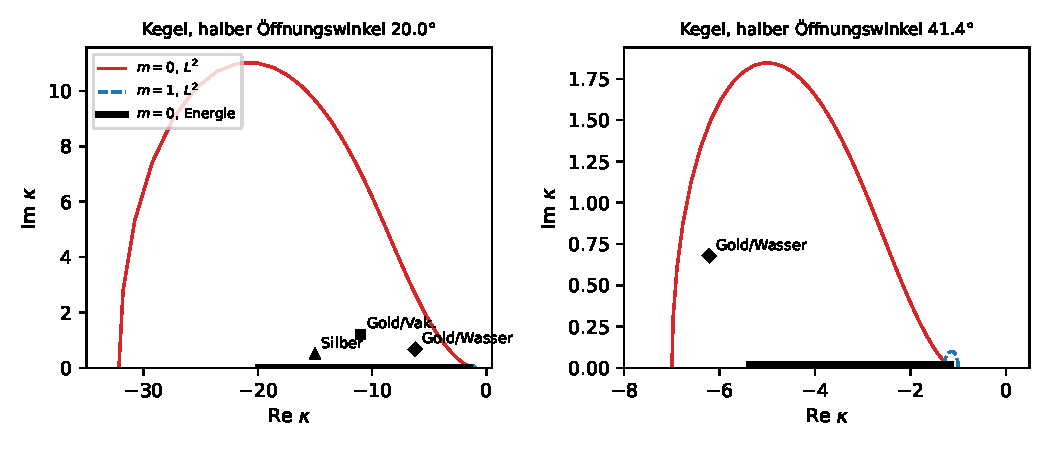
\includegraphics[width=\textwidth]{fig_cone.pdf}
\caption{Kritische Mengen an Kegelspitzen. Rot: $m=0$ in $L^2$ (komplexe Schleife);
schwarzer Balken: $m=0$ in der Energie-Theorie (reelles Intervall); blau: $m=1$ in $L^2$.}
\label{fig:cone}
\end{figure}

\paragraph{Einordnung.} Windungszahl der Schleife $m=0$ in $L^2$ um den Kontrast.
$1$ heißt „innerhalb“:
\begin{center}\small
\begin{tabular}{lccc}
\toprule
$\kappa$ & $\theta_0=20^\circ$ & $41{,}4^\circ$ & $60^\circ$\\
\midrule
Gold/Vakuum $-11+1{,}2i$ & 1 & 0 & 0\\
Silber/Vakuum $-15+0{,}5i$ & 1 & 0 & 0\\
Gold/Wasser $-6{,}2+0{,}68i$ & 1 & 1 & 0\\
$-3+0{,}3i$ & 1 & 1 & 0\\
\bottomrule
\end{tabular}
\end{center}
Die Singulärexponenten im Streifen $-\tfrac12<\operatorname{Re}\nu<0$ (per Nullstellensuche)
und die daraus nötigen Gewichte:
\begin{center}\small
\begin{tabular}{lcc}
\toprule
Fall & $\nu$ & nötiges $\beta>-\operatorname{Re}\nu$\\
\midrule
Gold/Vakuum, $20^\circ$ & $-0{,}393-0{,}792i$ & $0{,}39$\\
Silber/Vakuum, $20^\circ$ & $-0{,}465-0{,}491i$ & $0{,}47$\\
Gold/Wasser, $41{,}4^\circ$ & $-0{,}079-0{,}116i$ & $0{,}08$\\
$-3+0{,}3i$, $41{,}4^\circ$ & $-0{,}343-1{,}070i$ & $0{,}34$\\
\bottomrule
\end{tabular}
\end{center}

\paragraph{Konormalsymbol von $T_1$ an der Spitze.} Die Rechnung oben liefert die
kritische Menge des \emph{physikalischen} quasistatischen Problems. Für $T_1$ selbst
wird die Zerlegungsbedingung direkt geprüft (\texttt{cone\_dirac.py}). Für Mode $m$ und
Grad $\nu$ werden die Hardy-Räume $R_\pm$ von den Spuren homogener monogener Funktionen
$F=(\nabla H)\,c$ am Meridianpunkt aufgespannt, mit
$H=r^\nu P_\nu^{|\mu|}(\pm\cos\theta)e^{i\mu\varphi}$ harmonisch. $c$ liegt im Eigenraum der
Drehung zum Index $\mu-m\in\{-1,0,1\}$; das sichert die Kovarianz, und die Indizes sind
numerisch geprüft. Man erhält $\dim R_\pm=4$ in allen Fällen und bei $\kappa=1$ die
Zerlegung $\mathbb{C}^8=R_+\oplus R_-$. Kritisch ist $R_+\cap JR_-\ne\{0\}$. Das ist ein
Laurent-Polynom in $s=\sqrt\kappa$, dessen Nullstellen per FFT bestimmt werden, unter
Beachtung des Hauptzweigs.

\begin{satz}[Konormalsymbol an Kegelspitzen]\label{satz:kegelT1}\status{numerisch belegt}
Mit Standardwahl sind die kritischen Kontraste des Konormalsymbols von $T_1$ an der
Spitze eines Kreiskegels genau die physikalischen $\kappa(\nu,m)$. Die Hilfsgrade
erzeugen keine zusätzlichen kritischen Kontraste.
\end{satz}
\noindent\emph{Nachweis.} 54 Fälle: $\theta_0\in\{20^\circ,60^\circ,120^\circ\}$,
$m\in\{0,1,3\}$, $\operatorname{Re}\nu\in\{0,-\tfrac14\}$ und
$\tau\in\{0{,}2;0{,}9;2{,}5\}$, dazu $\theta_0=41{,}4^\circ$ mit $m\le2$. Die einzige
nichttriviale Nullstelle stimmt jeweils mit $\kappa(\nu,m)$ auf $9\cdot10^{-13}$ überein;
die übrigen Nullstellen sind die Ausnahmewerte $\kappa=0$ und $\kappa=\infty$. Das
duale Problem mit $W=1$ ist an der Spitze stets regulär, denn bei $\kappa=1$ zerfällt
$\mathbb{C}^8$ wie gesagt direkt. Damit ist die kritische Menge der Zerlegung auch die
von $T_1$.

\paragraph{Folgerungen.} Damit gilt die Übereinstimmung von $T_1$ mit dem
physikalischen Kriterium, die an Kanten bewiesen ist (Satz~\ref{satz:faktor}), auch an
Kegelspitzen. Es folgt:
\begin{enumerate}[leftmargin=*]
  \item Anders als an Kanten reicht die $L^2$-kritische Menge an \emph{spitzen}
    Kegeln weit ins Metallische: bis $-32$ bei $\theta_0=20^\circ$. Gold und Silber in
    Vakuum liegen dort innerhalb. Scharfe Metallspitzen, wie sie in der
    spitzenverstärkten Spektroskopie vorkommen, verlangen deshalb auch für
    Standardmetalle gewichtete Räume.
  \item Für Silber an einer $20^\circ$-Spitze liegt das nötige Gewicht mit
    $\beta>0{,}47$ nahe an der Muckenhoupt-Grenze $\tfrac12$. Nach
    Abschnitt~\ref{sec:geo} sind dann große Stabilitätskonstanten und langsame
    Konvergenz zu erwarten. Physikalisch liegt das verlustfreie Silber im
    Energie-Intervall $[-19{,}95,-1]$ dieser Spitze, und der Verlust hält es nur knapp
    heraus.
  \item Für die Würfelecke ist der Vergleichskegel ($41{,}4^\circ$) unkritischer als
    die rechtwinklige Kante (Endpunkt $-7$ statt $-5{,}83$). Gold/Wasser liegt an der Kante knapp außerhalb, am
    Vergleichskegel innerhalb der Schleife. Das ist nur ein grober Hinweis; die echte
    Würfelecke erfordert ein Mellin-Symbol auf dem sphärischen Dreieck.
\end{enumerate}

\paragraph{Grenzen der Analyse.} Behandelt ist das Konormalsymbol, also eine
\emph{notwendige} Bedingung. Nicht behandelt sind die Kantenoperatoren für
$\xi_3\neq0$, die Ecken des Würfels (3D-Kegel, Mellin-Symbol auf der Sphäre),
magnetische Kontraste und Frequenzkorrekturen. Die Ecken können die kritische Menge
nur vergrößern.

%======================================================================
\section{Teil V: Eindeutigkeit mit Standardwahl}\label{sec:teil5}
%======================================================================

Abschnitt~\ref{sec:faktor} zeigt, dass an Kanten die Standardwahl
$a_{\mathrm H}=\sqrt{r_\mu}$, $b_{\mathrm H}=\sqrt{r_\varepsilon}$ zu verwenden ist, mit
den Wurzeln je Medium: $\sqrt{r_\mu}=\sqrt{\mu_1}/\sqrt{\mu_2}$. Für sie fehlte bisher ein
Eindeutigkeitsbeweis. Die Idee: Die Hilfskomponenten werden nicht, wie in
Satz~\ref{satz:eind}, in eine gemeinsame Energie eingebaut, sondern
\emph{entkoppelt}. Die Standardwahl macht die Hilfspotentiale stetig, und die
Maxwell-Struktur erzwingt dann auch die Stetigkeit ihrer Normalableitungen.

\begin{lemma}[Hilfsanteil in Feldgrößen]\label{lem:hilfsfeld}\status{bewiesen, symb.\ verif.}
Im Medium $(\varepsilon,\mu)$ sei $G = G_M + \frac1{ik}(\nabla+ik)(\alpha+I\beta)$ die
Zerlegung aus Satz~\ref{satz:zerlegung}, und
$\varphi:=\alpha/\sqrt\mu$, $\psi:=\beta/\sqrt\varepsilon$. Dann tragen die Hilfsanteile
zu den unskalierten Feldern
\[
  \mvec{E}_{\mathrm{aux}} = \frac{\nabla\varphi}{i\omega\varepsilon},\qquad
  \mvec{H}_{\mathrm{aux}} = \frac{\nabla\psi}{i\omega\mu}
\]
bei, und $\varphi,\psi$ sind Helmholtz-Lösungen zur Wellenzahl $k$.
\end{lemma}
\begin{proof}
Der Grad-1-Anteil von $\frac1{ik}(\nabla+ik)\alpha$ ist $\nabla\alpha/(ik)$, der
Grad-2-Anteil von $\frac1{ik}(\nabla+ik)(I\beta)$ ist $I\nabla\beta/(ik)$. Mit
$k=\omega\sqrt\varepsilon\sqrt\mu$ folgt die Behauptung
(\texttt{check\_standard\_uniqueness.py}).
\end{proof}

\begin{satz}[Eindeutigkeit mit Standardwahl]\label{satz:eindstd}\status{bewiesen, reguläre Lösungen}
Sei $\omega>0$, das Außenmedium verlustfrei ($\varepsilon_2,\mu_2>0$) und das
Innenmedium passiv mit
\begin{equation}\label{eq:imk}
  \operatorname{Im}(\varepsilon_1\mu_1)\ \ge\ 0 .
\end{equation}
Mit der Standardwahl hat das homogene Transmissionsproblem \eqref{eq:trans} auf dem
vollen Raum nur die triviale Lösung.
\end{satz}

\begin{proof}
Sei $G_1$ innen, $G_2$ außen strahlend, $h_1=Jh_2$. Wir zerlegen
$G_j = G_{M,j} + \frac1{ik_j}(\nabla+ik_j)u_j$ und setzen $\varphi_j,\psi_j$ wie in
Lemma~\ref{lem:hilfsfeld}.

\emph{Schritt 1 (Hilfspotentiale stetig).} Auf den Graden 0 und 3 wirkt $J$ mit den
Faktoren $\sqrt{\mu_1}/\sqrt{\mu_2}$ und $\sqrt{\varepsilon_1}/\sqrt{\varepsilon_2}$.
Die Bedingungen $\alpha_1 = \frac{\sqrt{\mu_1}}{\sqrt{\mu_2}}\alpha_2$,
$\beta_1 = \frac{\sqrt{\varepsilon_1}}{\sqrt{\varepsilon_2}}\beta_2$ sind also genau
$\varphi_1=\varphi_2$ und $\psi_1=\psi_2$ auf $\Gamma$. Insbesondere stimmen die
Oberflächengradienten $\nabla_\Gamma\varphi$, $\nabla_\Gamma\psi$ beidseitig überein.

\emph{Schritt 2 (Tangentialsprünge der Maxwell-Anteile).} Auf den Graden 1 und 2
bewirkt $J$ die Stetigkeit von $\mvec{E}_T,\mvec{H}_T,\varepsilon E_n,\mu H_n$ der
\emph{Gesamt}felder (Lemma~\ref{lem:J}). Mit Lemma~\ref{lem:hilfsfeld} folgt
\[
  [\mvec{E}_{M,T}] = -\frac{1}{i\omega}\Big(\frac1{\varepsilon_1}-\frac1{\varepsilon_2}\Big)\nabla_\Gamma\varphi,
  \qquad
  [\mvec{H}_{M,T}] = -\frac{1}{i\omega}\Big(\frac1{\mu_1}-\frac1{\mu_2}\Big)\nabla_\Gamma\psi,
\]
mit $[f]=f_1-f_2$. Die Sprünge der tangentialen Maxwell-Felder sind also
Oberflächengradienten mit konstantem Vorfaktor.

\emph{Schritt 3 (Normalableitungen stetig).} Für Maxwell-Felder gilt
$\varepsilon E_{M,n} = \frac{i}{\omega}\,\n\cdot\nabla\times\mvec{H}_M =
\frac{i}{\omega}\operatorname{curl}_\Gamma\mvec{H}_{M,T}$. Damit ist
\[
  [\varepsilon E_{M,n}] = \tfrac{i}{\omega}\operatorname{curl}_\Gamma[\mvec{H}_{M,T}]
  = \text{const}\cdot\operatorname{curl}_\Gamma\nabla_\Gamma\psi = 0,
\]
analog $[\mu H_{M,n}]=0$. Die Normalbedingung der Gesamtfelder lautet nach
Lemma~\ref{lem:hilfsfeld}
$[\varepsilon E_{M,n}] + \frac{1}{i\omega}[\partial_n\varphi] = 0$. Also ist
$[\partial_n\varphi]=0$, und ebenso $[\partial_n\psi]=0$.

\emph{Schritt 4 (Hilfspotentiale verschwinden).} $\varphi$ löst
$\Delta\varphi+k(\mvec{x})^2\varphi=0$ stückweise, strahlt nach außen, und Wert und
Normalableitung sind über $\Gamma$ stetig. Die Green-Formel auf $B_R$ ergibt daher ohne
Grenzflächenterme
\[
  \operatorname{Im}\int_{S_R}\partial_r\varphi\,\bar\varphi\,dS
  = -\omega^2\operatorname{Im}(\varepsilon_1\mu_1)\int_\Omega|\varphi|^2 \le 0 .
\]
Mit der Sommerfeld-Bedingung ist die linke Seite
$k_2\int_{S_R}|\varphi|^2+o(1)$. Also gilt $\int_{S_R}|\varphi|^2\to0$, nach dem
Rellich-Lemma ist $\varphi\equiv0$ außen, und wegen verschwindender Cauchy-Daten auf
$\Gamma$ (eindeutige Fortsetzung) auch innen. Ebenso ist $\psi\equiv0$. Damit
verschwinden $\alpha,\beta$ und der gesamte Hilfsanteil.

\emph{Schritt 5 (Maxwell-Anteil).} Nun ist $G_j=G_{M,j}$, und $J$ liefert die
physikalischen Transmissionsbedingungen. Die klassische Eindeutigkeit folgt aus dem
Poynting-Satz ($\operatorname{Re}\int_{S_R}\xh\cdot\mvec{E}\times\overline{\mvec{H}}
= -\omega\int_\Omega(\operatorname{Im}\varepsilon_1|\mvec{E}|^2+\operatorname{Im}\mu_1|\mvec{H}|^2)\le0$)
und dem Rellich-Lemma für jedes passive Innenmedium. Also ist $G_2\equiv0$,
$h_1=Jh_2=0$ und $G_1=\mathcal{C}_{k_1}h_1=0$.
\end{proof}

\begin{bemerkung}[Tragweite]\label{bem:eindstd}
\begin{enumerate}[leftmargin=*]
  \item Bedingung \eqref{eq:imk} ist für alle \emph{nichtmagnetischen} passiven
    Medien erfüllt ($\mu_1>0$, $\operatorname{Im}\varepsilon_1\ge0$), also auch für
    verlustfreie und verlustbehaftete Metalle. Sie kann nur verletzt sein, wenn
    $\operatorname{Re}\varepsilon_1<0$ \emph{und} $\operatorname{Im}\mu_1>0$ zugleich
    gilt (oder umgekehrt). Dann liefert Schritt~4 kein Vorzeichen; ob die Aussage
    dort trotzdem gilt, ist offen.
  \item Der Beweis benötigt nur, dass Green- und Poynting-Formel für die
    Lösungen gelten, also lokal endliche Energie. An Kanten sind die Randspuren in
    $L^2(r^{2\beta})$ mit $\beta<\tfrac12$. Die Felder verhalten sich dann wie
    $r^{a-1}$ mit $\operatorname{Re}a>\tfrac12-\beta>0$, sind lokal quadratintegrierbar,
    und die Flüsse sind integrabel. Die Hilfspotentiale sind nach
    Korollar~\ref{kor:faktor} an Kanten nicht singulär: Ihre Blöcke sind für die
    Standardwahl trivial. Die Argumentation überträgt sich also auf die gewichteten
    Räume aus Abschnitt~\ref{sec:exponenten}; eine vollständige Ausarbeitung der
    Spurregularität auf Lipschitz-Rändern steht aus.
  \item Der Unterschied zur Energiewahl: Dort wurde ein gemeinsamer Fluss für Maxwell-
    und Hilfsanteile konstruiert, der nur für eine spezielle, an Kanten ungeeignete
    Parameterwahl über $\Gamma$ stetig ist. Hier entkoppeln die Hilfsanteile
    vollständig, und zwar gerade \emph{wegen} der Standardwahl. Das ist dieselbe
    Struktur, die im Konormalsymbol die Hilfsblöcke trivial macht.
\end{enumerate}
\end{bemerkung}

\begin{korollar}[Invertierbarkeit von $T_1$ mit Standardwahl]\label{kor:T1std}
\status{bewiesen, glatter Rand}
Unter den Voraussetzungen von Satz~\ref{satz:eindstd}, für glatten Rand und
$\varepsilon_1\neq-\varepsilon_2$, $\mu_1\neq-\mu_2$ ist $T_1$ mit der Standardwahl ein
Isomorphismus auf $L^2(\Gamma;\clc)$. An Rändern mit Kanten gilt die Injektivität in
$L^2(r^{2\beta})$ (Bemerkung~\ref{bem:eindstd}). Zusammen mit der Fredholm-Eigenschaft
wäre $T_1$ dort invertierbar; diese ist bisher nur auf der Ebene des
Konormalsymbols gezeigt (Abschnitt~\ref{sec:exponenten}).
\end{korollar}
\begin{proof}
Injektivität aus Satz~\ref{satz:eindstd}, Lemma~\ref{lem:TW} und
Satz~\ref{satz:dualW1}. Letzterer verwendet nur den Fluss $\mvec{j}[G]$ und gilt für
jede Parameterwahl. Fredholm vom Index~0 nach Korollar~\ref{kor:T1}.
\end{proof}

Damit ist Vermutung~\ref{verm:inj2} für die Standardwahl bewiesen, für alle Medien
mit \eqref{eq:imk}. Die Energiewahl wird nicht mehr benötigt. Die numerischen Befunde
passen dazu: Hilfsanteile auf Residuumsniveau in der Streudemo, keine
Hilfs-Einbrüche auf Kugel und Torus.

%======================================================================
\section{Teil VI: Chirale Grenzflächen (Schritt 1.6, Fortsetzung)}\label{sec:teil6}
%======================================================================

Innenmedium: Pasteur-Medium $(\varepsilon_1,\mu_1,\chi_1)$ mit
$\mvec{D}=\varepsilon\mvec{E}+i\chi\mvec{H}$, $\mvec{B}=\mu\mvec{H}-i\chi\mvec{E}$;
Außenmedium achiral. Für den Hauptteil ist das Außenmedium auf Vakuum normiert.

\begin{lemma}[Chirale Transmissionsabbildung]\label{lem:Jchiral}\status{bewiesen, num.\ verif.}
Mit $F_j=\sqrt{\varepsilon_j}\mvec{E}+I\sqrt{\mu_j}\mvec{H}$ bleiben die Tangentialfaktoren
aus Lemma~\ref{lem:J} unverändert. Die Normalanteile $(e_n,h_n)=(\sqrt\varepsilon E_n,\sqrt\mu H_n)$
koppeln über
\[
  \begin{pmatrix}e_n\\h_n\end{pmatrix}_1 = D_1C_1^{-1}C_2D_2^{-1}\begin{pmatrix}e_n\\h_n\end{pmatrix}_2,
  \qquad C_j=\begin{pmatrix}\varepsilon_j & i\chi_j\\ -i\chi_j & \mu_j\end{pmatrix},\quad
  D_j=\operatorname{diag}(\sqrt{\varepsilon_j},\sqrt{\mu_j}).
\]
$J$ mischt also den vektoriellen Normalanteil $\n$ mit dem bivektoriellen $I\n$. Für
$\chi_j=0$ ergibt sich Lemma~\ref{lem:J}.
\end{lemma}

\noindent Die Prüfung erfolgt an der exakten Fresnel-Lösung (\texttt{chiral\_J.py}): Im
chiralen Halbraum überlagern sich zwei Helizitäts-Eigenwellen
$P_\pm(1+\mvec{d})\mvec{c}\,e^{ik_\pm\mvec{d}\cdot\mvec{x}}$ mit transversalem
$\mvec{c}$ ($\mvec{d}\cdot\mvec{c}=0$, sonst entstehen Hilfskomponenten), außen die
reflektierten TE- und TM-Wellen. Nach Lösen der vier Tangentialbedingungen ist
$|h_1-Jh_2|/|h_1|\le6\cdot10^{-16}$ für drei Einfallswinkel und die Medien
$(\varepsilon_1,\mu_1,\chi_1)=(2{,}25;\,1;\,0{,}1)$, $(2{,}25;\,1;\,0{,}4)$,
$(-11+1{,}2i;\,1;\,0{,}3)$ und $(3;\,1{,}5;\,0{,}2+0{,}05i)$. Die konstitutiven Normalbedingungen sind unabhängig davon auf
$10^{-14}$ erfüllt.

\begin{satz}[Hauptsymbol, glatter Rand]\label{satz:chiralsym}\status{symbolisch}
Für das Transmissionsproblem mit chiralem Innenmedium und Vakuum außen gilt
\begin{gather*}
  \det[\,J^{-1}\operatorname{ran}p_+,\ \operatorname{ran}p_-\,]\ \propto\
  \frac{(\varepsilon_1+1)(\mu_1+1)-\chi_1^2}{\varepsilon_1\mu_1},\\
  \det\sigma(T_1)\ \propto\ \frac{\varepsilon_1\mu_1\big[(\varepsilon_1+1)(\mu_1+1)-\chi_1^2\big]}{\varepsilon_1\mu_1-\chi_1^2}.
\end{gather*}
Die Ausnahmemenge $\{\varepsilon_1=-1\}\cup\{\mu_1=-1\}$ wird zu
$(\varepsilon_1+1)(\mu_1+1)=\chi_1^2$. Für $\mu_1=1$ verschiebt sich die glatte
Plasmonbedingung also nach $\varepsilon_1=-1+\chi_1^2/2$. Zusätzlich wird $J$ für
$\varepsilon_1\mu_1=\chi_1^2$ singulär, also bei $k_-=0$.
\end{satz}
\noindent\emph{Nachweis.} SymPy, mit $\sqrt{\varepsilon_1},\sqrt{\mu_1}$ als Symbolen
(\texttt{chiral\_symbol.py}). Der Chiralitätsterm $\omega\chi I$ der
Dirac-Gleichung ist von nullter Ordnung und geht nicht ins Hauptsymbol ein. Die
Chiralität wirkt im Symbol ausschließlich über $J$.

\begin{satz}[Konormalsymbol an einer Ecke]\label{satz:chiralecke}\status{40-stellig verifiziert}
Die Hilfsblöcke aus Lemma~\ref{lem:block} bleiben ungekoppelt. TM- und TE-Block
koppeln über die Normalanteile, und für ihre gemeinsame Determinante gilt
\[
  \det\nolimits_{E_\parallel\oplus H_\parallel}\ =\ \frac{\varepsilon_1\mu_1}{16\,(\varepsilon_1\mu_1-\chi_1^2)^2}\Big(\mathcal{A}-\mathcal{B}\,S(a)^2+\mathcal{C}\,S(a)^4\Big)
\]
mit
\begin{align*}
  \mathcal{A} &= \big((1+\varepsilon_1)(1+\mu_1)-\chi_1^2\big)^2,\qquad
  \mathcal{C} = \big((1-\varepsilon_1)(1-\mu_1)-\chi_1^2\big)^2,\\
  \mathcal{B} &= 2(1+\varepsilon_1^2)(1+\mu_1^2) - 8\varepsilon_1\mu_1 + 4\chi_1^2(3-\varepsilon_1\mu_1) + 2\chi_1^4 .
\end{align*}
\end{satz}
\noindent\emph{Nachweis.} Die Nebenblöcke zu den Hilfsgraden sind exakt null. Für
$\alpha=\pi/2$ wurde $-c_1/c_0\cdot\mathcal{A}$ an 45 zufälligen komplexen Parametersätzen
mit allen Monomen $\varepsilon^i\mu^j\chi^{2k}$ ($i,j,k\le2$) angepasst. Das Ergebnis
sind ganzzahlige Koeffizienten mit Rest $10^{-10}$. Für $\alpha\in\{\pi/3,\,1{,}3,\,2\pi/3\}$
sagt die Formel die Determinante an einem unabhängigen vierten Punkt auf $5\cdot10^{-13}$
vorher (\texttt{chiral\_corner.py}). Mit exakten Mellin-Einträgen und 40 Stellen
stimmen Formel und Vorfaktor für allgemeine $(a,\alpha)$ und zwei komplexe Medien auf
$10^{-40}$ (\texttt{chiral\_corner\_exact.py}). Kontrollen: Für $\chi_1=0$ ist
$\mathcal{A}-\mathcal{B}S^2+\mathcal{C}S^4=\hat g(\varepsilon_1)\hat g(\mu_1)$ wie in
Satz~\ref{satz:faktor}, und im glatten Grenzfall $S\to0$ bleibt
$\mathcal{A}=0$, wie in Satz~\ref{satz:chiralsym}. Ein exakter symbolischer
Beweis (wie für Satz~\ref{satz:faktor}) steht für den gekoppelten $8\times8$-Block aus.

\begin{figure}[ht]
\centering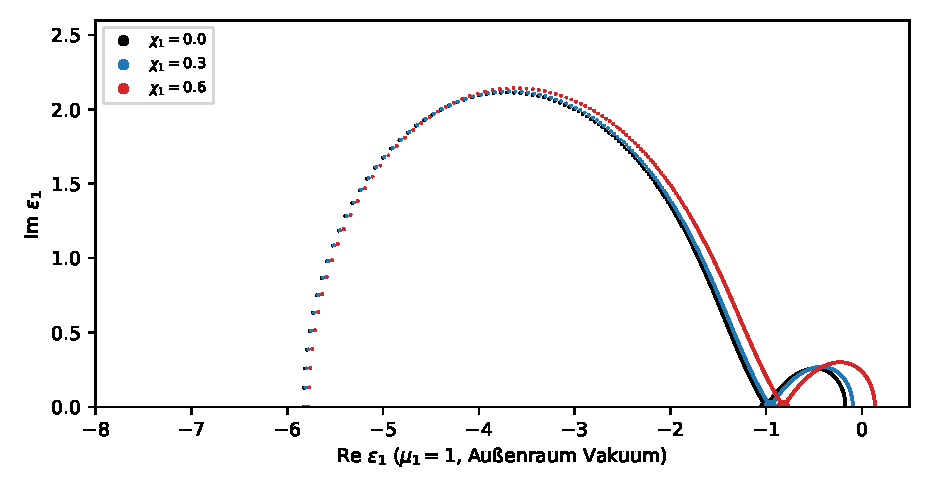
\includegraphics[width=0.92\textwidth]{fig_chiral_corner.pdf}
\caption{Kritische Mengen in der $\varepsilon_1$-Ebene an einer rechtwinkligen Kante
($L^2$, $\mu_1=1$) für $\chi_1=0;\ 0{,}3;\ 0{,}6$.}
\label{fig:chiralecke}
\end{figure}

\paragraph{Folgerungen.} Die Verschiebung ist von der Ordnung $\chi_1^2$
(Abbildung~\ref{fig:chiralecke}). Die reellen Endpunkte der Schleifen liegen bei
$-5{,}83$ und $-0{,}17$ für $\chi_1=0$, bei $-5{,}82$ und $-0{,}09$ für $\chi_1=0{,}3$
und bei $-5{,}78$ und $+0{,}14$ für $\chi_1=0{,}6$. Für natürliche chirale Medien
($|\chi|\ll1$) ist der Effekt vernachlässigbar. Für stark chirale Metamaterialien
reicht die kritische Menge dagegen bis zu \emph{positiven} $\varepsilon_1$. Das ist
der Bereich $\varepsilon_1\mu_1<\chi_1^2$, in dem eine Helizität evaneszent wird
(„chirale Nullbrechung“, Bezeichnung zu prüfen). Die Aussagen aus Teil IV über
Gewichte und Standardwahl gelten sinngemäß, da die Hilfsblöcke unverändert trivial
sind.

\subsection{Eindeutigkeit für chirale Innenmedien}\label{sec:chiraleind}

\begin{lemma}[Helizitätsweise Zerlegung]\label{lem:chiralzerl}\status{bewiesen, symb.\ verif.}
Sei $(\nabla - ik)G = \omega\chi IG$ im Pasteur-Medium, $k_\pm=\omega(\sqrt{\varepsilon}\sqrt{\mu}\mp\chi)\neq0$.
Dann ist
\[
  G = G_M + \sum_\pm \tfrac{1}{ik_\pm}(\nabla+ik_\pm)(\gamma_\pm P_\pm),
\]
mit Helmholtz-Lösungen $\gamma_\pm$ zu $k_\pm$ und einem chiralen Maxwell-Feld $G_M$ (Grade 1, 2).
Für die Hilfsanteile gilt $\alpha=\tfrac12(\gamma_++\gamma_-)$, $\beta=\tfrac i2(\gamma_+-\gamma_-)$,
und mit $\varphi=\alpha/\sqrt\mu$, $\psi=\beta/\sqrt\varepsilon$
\[
  \mvec{D}_{\mathrm{aux}} = \varepsilon\mvec{E}_{\mathrm{aux}}+i\chi\mvec{H}_{\mathrm{aux}} = \frac{\nabla\varphi}{i\omega},\qquad
  \mvec{B}_{\mathrm{aux}} = \mu\mvec{H}_{\mathrm{aux}}-i\chi\mvec{E}_{\mathrm{aux}} = \frac{\nabla\psi}{i\omega}.
\]
\end{lemma}
\begin{proof}
Satz~\ref{satz:zerlegung} wird auf $P_\pm G$ angewendet, die nach Satz~\ref{satz:chiral}
die Dirac-Gleichung zu $k_\pm$ lösen. Der Grad-0-plus-3-Anteil von $P_\pm G$ ist
$P_\pm u = (\alpha\mp i\beta)P_\pm =: \gamma_\pm P_\pm$, wegen $IP_\pm=\mp iP_\pm$. Die
Feldidentitäten folgen aus $k_\pm = \omega(\sqrt{\varepsilon\mu}\mp\chi)$, denn der
Faktor $(\sqrt{\varepsilon\mu}\mp\chi)/k_\pm = 1/\omega$ ist für beide Helizitäten gleich
(\texttt{check\_chiral\_uniqueness.py}). Für $\chi=0$ ergibt sich
Lemma~\ref{lem:hilfsfeld}.
\end{proof}

Die Identität für $\mvec{D}_{\mathrm{aux}},\mvec{B}_{\mathrm{aux}}$ ist der Kern: In den
Größen, die die Grenzflächenbedingungen tatsächlich enthalten, verschwindet die
Chiralität aus dem Hilfsanteil.

\begin{satz}[Eindeutigkeit, chirales Innenmedium]\label{satz:eindchiral}\status{bewiesen, reguläre Lösungen}
Sei $\omega>0$, das Außenmedium achiral und verlustfrei, das Innenmedium ein passives
Pasteur-Medium ($\operatorname{Im}\varepsilon_1,\operatorname{Im}\mu_1\ge0$,
$(\operatorname{Im}\chi_1)^2\le\operatorname{Im}\varepsilon_1\operatorname{Im}\mu_1$) mit
\begin{equation}\label{eq:imkpm}
  \operatorname{Im}(k_+^2)\ge0\quad\text{und}\quad\operatorname{Im}(k_-^2)\ge0 .
\end{equation}
Mit der Standardwahl und der chiralen Abbildung $J$ aus Lemma~\ref{lem:Jchiral} hat das
homogene Transmissionsproblem nur die triviale Lösung.
\end{satz}
\begin{proof}
\emph{Schritte 1 bis 3} verlaufen wie in Satz~\ref{satz:eindstd}. Die
Grad-0/3-Bedingungen der Standardwahl ergeben $[\varphi]=[\psi]=0$. Die
Tangentialsprünge der Maxwell-Anteile sind Oberflächengradienten. Für chirale
Maxwell-Felder gilt $D_{M,n}=\frac{i}{\omega}\operatorname{curl}_\Gamma\mvec{H}_{M,T}$ und
$B_{M,n}=\frac{1}{i\omega}\operatorname{curl}_\Gamma\mvec{E}_{M,T}$, also
$[D_{M,n}]=[B_{M,n}]=0$. Die Normalbedingungen aus $J$ (Stetigkeit von $D_n, B_n$)
liefern mit Lemma~\ref{lem:chiralzerl} dann $[\partial_n\varphi]=[\partial_n\psi]=0$.

\emph{Schritt 4 (neu).} Innen sind $\varphi,\psi$ keine Helmholtz-Lösungen, wohl aber
$\gamma_\pm$. Die gewichtete Randform
\[
  W := |\mu_1|\,\partial_n\varphi\,\bar\varphi + |\varepsilon_1|\,\partial_n\psi\,\bar\psi
\]
ist über $\Gamma$ stetig. Innen gilt punktweise
$W=\tfrac12\big(\partial_n\gamma_+\bar\gamma_++\partial_n\gamma_-\bar\gamma_-\big)$; die
Kreuzterme heben sich genau bei diesen Gewichten auf (symbolisch geprüft). Die
Green-Formel ergibt innen
\[
  \operatorname{Im}\int_\Gamma W = -\tfrac12\sum_\pm\operatorname{Im}(k_\pm^2)\int_\Omega|\gamma_\pm|^2\ \le\ 0,
\]
und außen, wo $\varphi,\psi$ strahlende Helmholtz-Lösungen zu reellem $k_2$ sind,
\[
  \operatorname{Im}\int_\Gamma W = k_2\Big(|\mu_1|\int_{S_R}|\varphi|^2+|\varepsilon_1|\int_{S_R}|\psi|^2\Big)+o(1)\ \ge\ 0 .
\]
Also verschwinden die Fernfelder, außen ist $\varphi=\psi=0$, und die
Cauchy-Daten von $\gamma_\pm$ auf $\Gamma$ sind null. Nach eindeutiger Fortsetzung ist
$\gamma_\pm=0$ innen.

\emph{Schritt 5.} Der verbleibende Maxwell-Anteil erfüllt das physikalische
chirale Transmissionsproblem. Der Poynting-Satz liefert
$\operatorname{Re}\nabla\cdot(\mvec{E}\times\overline{\mvec{H}})
= -\omega\big[\operatorname{Im}\varepsilon|\mvec{E}|^2+\operatorname{Im}\mu|\mvec{H}|^2
+2\operatorname{Im}\chi\,\operatorname{Im}(\mvec{E}\cdot\overline{\mvec{H}})\big]\le0$
unter der Passivitätsbedingung. Mit dem Rellich-Lemma folgt die Eindeutigkeit.
\end{proof}

\paragraph{Tragweite der Bedingung \eqref{eq:imkpm}.} Sie lautet
$\operatorname{Im}(\varepsilon_1\mu_1)+\operatorname{Im}(\chi_1^2)\ge2\,|\operatorname{Im}(\chi_1\sqrt{\varepsilon_1\mu_1})|$
und ist für $\chi_1=0$ genau \eqref{eq:imk}. Werte von $\operatorname{Im}(k_\pm^2)/\omega^2$:
\begin{center}\small
\begin{tabular}{lcc}
\toprule
$(\varepsilon_1,\mu_1,\chi_1)$ & $\operatorname{Im}k_+^2$ & $\operatorname{Im}k_-^2$\\
\midrule
$(2{,}25;\ 1;\ 0{,}1)$ & $0$ & $0$\\
$(2{,}25+0{,}01i;\ 1;\ 0{,}1)$ & $0{,}009$ & $0{,}011$\\
$(-11+1{,}2i;\ 1;\ 0{,}01)$ & $1{,}13$ & $1{,}27$\\
$(-11+1{,}2i;\ 1;\ 0{,}3)$ & $-0{,}79$ & $3{,}19$\\
$(3+0{,}5i;\ 1{,}5+0{,}2i;\ 0{,}2+0{,}05i)$ & $1{,}03$ & $1{,}71$\\
\bottomrule
\end{tabular}
\end{center}
Verlustfreie und schwach dämpfende chirale Dielektrika sind abgedeckt, ebenso
Metalle mit schwacher Chiralität (für Gold, $\varepsilon=-11+1{,}2i$, etwa bis
$|\chi_1|\lesssim0{,}18$). Nicht abgedeckt sind stark chirale Metalle und verlustfreie
chirale Metalle mit $\chi_1\neq0$. Dort hat eine Helizität $\operatorname{Im}k^2<0$.
Die Gewichte in $W$ sind durch die Aufhebung der Kreuzterme festgelegt; der Beweis
lässt sich also nicht durch eine andere Gewichtung retten. Ob die Aussage dort
trotzdem gilt, ist offen.

\paragraph{Chirales Außenmedium (glatter Rand).} Numerisch
(\texttt{chiral\_J.py} mit $\chi_2\ne0$, vier zufällige Mediensätze) ist das
Hauptsymbol genau dann singulär, wenn
\[
  (\varepsilon_1+\varepsilon_2)(\mu_1+\mu_2)=(\chi_1+\chi_2)^2
\]
(relatives $|\det|\le10^{-15}$ auf dieser Menge; die Variante mit $(\chi_1-\chi_2)^2$
trifft nicht). Das Pluszeichen folgt aus der gemeinsamen Vorzeichenkonvention
$\mvec{D}=\varepsilon\mvec{E}+i\chi\mvec{H}$ auf beiden Seiten. Eine reine Skalierung auf
Vakuum reicht hier also nicht aus.

\paragraph{Offen.} Chirale Außenmedien an Kanten,
der Fall stark chiraler Metalle in Satz~\ref{satz:eindchiral} und Tellegen-Medien
(Abschnitt~6).

%======================================================================
\section{Offene Punkte und Teil VII}\label{sec:offen}
%======================================================================

\begin{enumerate}[leftmargin=*]
  \item Schritt 1.5, Fortsetzung: die echte Würfelecke (Mellin-Symbol auf dem
    sphärischen Dreieck), Kantenoperatoren für $\xi_3\neq0$, Beweis von
    Satz~\ref{satz:kegelT1}.
  \item Eindeutigkeit mit Standardwahl ist bewiesen (Satz~\ref{satz:eindstd}).
    Offen sind der Fall $\operatorname{Im}(\varepsilon_1\mu_1)<0$ und die
    vollständige Spurregularität auf Lipschitz-Rändern (Bemerkung~\ref{bem:eindstd}).
  \item Gewichtete Formulierung $L^2(r^{2\beta})$ für $T_1$: Injektivität und
    Übertragung von Satz~\ref{satz:eind} auf Ränder mit Kanten.
  \item Übertragung der Eckblock-Vorkonditionierung (Abschnitt~\ref{sec:vorkond})
    auf 3D-Kanten, etwa als $\mathcal{H}$-LU von Kantenblöcken.
  \item Resonanzen im kritischen Intervall (Abschnitt~\ref{sec:resonanz}):
    belastbare Berechnung des diskreten Toeplitz-Symbols (Randverhalten bei
    $|z|\to1/q$), partielle Indizes, reflexionsfreie komplexe Streckung in $\log r$
    bzw.\ transparenter Eckabschluss.
  \item Chirale Medien: Eindeutigkeit ist für $\operatorname{Im}k_\pm^2\ge0$ bewiesen
    (Satz~\ref{satz:eindchiral}); offen sind stark chirale Metalle, ein exakter
    Beweis von Satz~\ref{satz:chiralecke}, chirale Außenmedien an Kanten und Tellegen-Medien.
  \item Eindeutigkeit mit der Standardwahl (Vermutung~\ref{verm:inj2}) oder
    Nachweis, dass die Standardwahl verzichtbar ist.
  \item Vergleich mit PMCHWT/Müller: Welche Kombination von \eqref{eq:trans}
    reproduziert welche klassische Formulierung.
  \item Übergang zu AP~2: Galerkin-Diskretisierung von $2(1+J)^{-1}T_1$ auf der
    Kugel und Test von H1 (Iterationszahlen unter $h$-Verfeinerung).
\end{enumerate}

\section*{Literatur (zu prüfen)}
{\small
Die folgenden Angaben stammen aus dem Gedächtnis und sind vor Verwendung zu
verifizieren.
\begin{itemize}[leftmargin=*]
  \item D.~Hestenes, G.~Sobczyk: \emph{Clifford Algebra to Geometric Calculus}, Reidel, 1984.
  \item C.~Doran, A.~Lasenby: \emph{Geometric Algebra for Physicists}, Cambridge UP, 2003.
  \item A.~Rosén: \emph{Geometric Multivector Analysis}, Birkhäuser, 2019.
  \item A.~Axelsson, R.~Grognard, J.~Hogan, A.~McIntosh: Harmonic analysis of
    Dirac operators on Lipschitz domains, in: \emph{Clifford Analysis and its
    Applications}, Kluwer, 2001.
  \item J.~Helsing, A.~Rosén: Dirac integral equations for dielectric and
    plasmonic scattering, \emph{Integral Equations Operator Theory}, 2021.
  \item R.~Coifman, A.~McIntosh, Y.~Meyer: L'intégrale de Cauchy définit un
    opérateur borné sur $L^2$ pour les courbes lipschitziennes, \emph{Ann.\ Math.}, 1982.
  \item D.~Colton, R.~Kress: \emph{Inverse Acoustic and Electromagnetic Scattering Theory}, Springer.
  \item J.-C.~Nédélec: \emph{Acoustic and Electromagnetic Equations}, Springer, 2001.
  \item K.-M.~Perfekt, M.~Putinar: The essential spectrum of the Neumann--Poincaré
    operator on a domain with corners, \emph{Arch.\ Ration.\ Mech.\ Anal.}, 2017.
  \item A.-S.~Bonnet-Ben Dhia, L.~Chesnel, P.~Ciarlet Jr.: T-coercivity for
    scalar interface problems between dielectrics and metamaterials,
    \emph{ESAIM: M2AN}, 2012.
  \item I.~Lindell, A.~Sihvola, S.~Tretyakov, A.~Viitanen: \emph{Electromagnetic
    Waves in Chiral and Bi-Isotropic Media}, Artech House, 1994.
\end{itemize}}


\section{Nachtrag: Resonanzfenster an Ecken und Kanten}\label{sec:fenster}
Dieser Abschnitt fasst die späteren Untersuchungen zum Resonanzfenster aus Teil~IV zusammen
(Prototypen \texttt{prototype/resonance}, Bericht \texttt{docs/results\_resonance\_window.md} im Repository
\texttt{PhotonPower/CliffordBem}).

\paragraph{Mechanismus.} Im Fenster hat die Kante einen Singulärexponenten $a=c-i\tau$ mit kleinem $c$
(rechter Winkel, $\kappa=-2{,}8+0{,}3i$: $a=0{,}151-0{,}238i$). Das Feld enthält in $\log r$ oszillierende
Wellen, die in die Ecke laufen; ihre Wellenlänge in $\ln r$ ist $2\pi/\tau\approx26$ (etwa 11 Dekaden). Bei
kleinem Verlust werden sie am innersten Element des gradierten Netzes reflektiert, daher die fehlende
Konvergenz in der Gradierungstiefe.

\paragraph{2D: gelöst.} Komplexe Streckung $r\mapsto r\,(r/r_0)^{i\theta}$ nahe der Ecke, analytisch
fortgesetzter Kern ($z\cdot z$ bilinear), Galerkin mit Testung durch das Konturintegral (ohne Konjugation):
\begin{itemize}[leftmargin=*]
  \item Das Vorzeichen von $\theta$ folgt aus dem physikalischen Exponenten ($\theta>0$); mit falschem
    Vorzeichen konvergiert das Verfahren in der Tiefe gegen eine unphysikalische Lösung.
  \item Die gestreckte Dichte liegt in $L^2$, wenn $c+\tau\theta>\tfrac12$.
  \item Ergebnis (Quadrat, $\kappa=-2{,}8+0{,}3i$): tiefenunabhängig auf $10^{-7}$, konvergent in der
    Gradierung, $\theta=2$ und $3$ stimmen auf $6\cdot10^{-4}$ überein; auch der verlustfreie Fall $\kappa=-2$ ist
    rechenbar (mit Energieabfluss in die Ecke), und $\kappa=-2+0{,}02i$ liegt nahe daran.
  \item Kollokation konvergiert dagegen nicht; sie war die zweite Ursache der Schwierigkeiten in Teil~IV.
\end{itemize}

\paragraph{3D.}
\begin{itemize}[leftmargin=*]
  \item An Kanten bleibt die Koordinate $t$ entlang der Kante reell; mit der Spiralstreckung liegt der
    transversale Anteil $w_T$ von $z\cdot z=(t_1-t_2)^2+w_T$ auch auf der negativen reellen Achse, der fortgesetzte
    Kern wird auf dem komplexen Rand singulär. Eine begrenzte Phase ($|\arg\tilde r|<\pi/2$) vermeidet das,
    dämpft aber höchstens um $e^{\tau\pi/2}$.
  \item Um Spitzen und Ecken ist eine isotrope Streckung aller Koordinaten zulässig.
  \item Weitere Versuche für Kanten, im 2D-Prototyp gegen die Streckungslösung geprüft: Eckelement mit
    $r^{a-1}$ (frei in allen Komponenten oder mit der exakten Mellin-Mode, deren Richtung die Referenzlösung mit
    $|\cos|=0{,}997$ bestätigt) und Absorber über elementweise $\operatorname{Im}\kappa$ in $J$. Beide sind nicht
    transparent; der Absorber müsste sich über Dutzende Dekaden erstrecken.
  \item Offene Wege: eine asymptotische diskrete DtN-Bedingung aus der Schichtstruktur (in tiefen Schichten mit
    $r\ll\Delta t$ wird das Kantenproblem asymptotisch zweidimensional) und Hardy-Raum-Ansätze.
\end{itemize}

\paragraph{Abgerundete Kanten.} Mit Rundungsradius $\rho$ ist der Rand glatt; im Fenster konvergiert die
3D-Rechnung dann monoton (Würfel, $\kappa=-2{,}8+0{,}3i$, $\rho=0{,}2$: $14{,}22\to13{,}31\to12{,}86$), hängt
aber stark von $\rho$ ab (etwa Halbierung der Extinktion von $\rho=0{,}4$ auf $0{,}2$). Für reale Nanowürfel ist
der Radius ein physikalischer Parameter.

\section{Nachtrag: Verschachtelte Gebiete und beschichtete Grenzflächen}\label{sec:schicht}

An Materialgrenzen liegen meist dünne Schichten (Oxide, Sulfide, Hüllen), die Amplitude und Phase des gestreuten
Lichts verändern. Dieser Nachtrag verallgemeinert $T_1$ auf Anordnungen aus mehreren geschlossenen Flächen, von
denen jede genau zwei Gebiete trennt (Kern--Schale, Mehrfachschichten, mehrere Körper, auch Einschlüsse).

\paragraph{Geometrie.} Gebiete $\Omega_0$ (Außenraum), $\Omega_1,\dots$ mit Medien $(\varepsilon_R,\mu_R,\chi_R)$;
glatte, paarweise disjunkte, geschlossene Flächen $\Gamma_s$ mit Außennormale $\n_s$, innen an $\Omega_{\mathrm{in}(s)}$,
außen an $\Omega_{\mathrm{out}(s)}$. Für ein Gebiet $R$ ist $\partial R=\bigcup\{\Gamma_s:R\in\{\mathrm{in}(s),
\mathrm{out}(s)\}\}$ und $\sigma_s=+1$, falls $R=\mathrm{in}(s)$, sonst $\sigma_s=-1$; die Außennormale von $R$ ist
$\sigma_s\n_s$. $E_R$ bezeichne den Randoperator zur Wellenzahl von $R$ auf $\partial R$, gebildet mit den Normalen
$\n_s$; da $\n$ im Kern linear eingeht, ist $E_R^\sigma u:=E_R(\sigma u)$ der Randoperator mit der Außennormale von
$R$.

\paragraph{Formulierung.} Unbekannt ist auf jeder Fläche die Außenspur $h_s$; die Innenspur ist $J_sh_s$ mit
$J_s=J(\n_s;\mathrm{in}(s),\mathrm{out}(s))$ (Lemma~\ref{lem:J}, chiral Lemma~\ref{lem:Jchiral}). Die Spur von $R$ ist
$u^R_s=J_sh_s$ für $R=\mathrm{in}(s)$ und $u^R_s=h_s$ sonst. Das System lautet
\begin{equation}\label{eq:schicht}
  \tfrac12\big[(1-E^\sigma_{\mathrm{out}(s)})u^{\mathrm{out}(s)}\big]_s
  +\tfrac12\big[(1-E^\sigma_{\mathrm{in}(s)})u^{\mathrm{in}(s)}\big]_s
  = h^{\mathrm{inc}}_s\,[\mathrm{out}(s)=0]\qquad\text{für alle }s .
\end{equation}
Für eine Fläche ist $E^\sigma_{\Omega_0}=-E_2$, $E^\sigma_{\Omega_1}=E_1$, und \eqref{eq:schicht} ist genau
$T_1h=E_2^+h+E_1^-Jh=h^{\mathrm{inc}}$.

\begin{prop}\label{prop:schicht}\status{bewiesen}
(a) Die Außenspuren des physikalischen Transmissionsproblems lösen \eqref{eq:schicht}.
(b) Sind die Flächen glatt und getrennt, so unterscheidet sich der Operator von \eqref{eq:schicht} von der
direkten Summe der lokalen $T_1$-Operatoren der einzelnen Flächen um einen kompakten Operator; er ist genau dann
Fredholm vom Index~0, wenn jede Fläche das Kriterium von Satz~\ref{satz:symbol} erfüllt.
\end{prop}
\begin{proof}
(a) Im beschränkten Gebiet $R$ ist das Feld durch die Cauchy-Formel aus $u^R$ darstellbar, also $(1-E^\sigma_R)u^R=0$
(Satz~\ref{satz:involution}). Im Außenraum gilt das für die Streuspur; die einfallende Welle ist im Komplement von
$\Omega_0$ regulär, dort ist $E^\sigma_{\Omega_0}u^{\mathrm{inc}}=-u^{\mathrm{inc}}$, also
$\tfrac12(1-E^\sigma_{\Omega_0})u^{\mathrm{inc}}=u^{\mathrm{inc}}$. (b) Die Anteile von $E_R$ zwischen verschiedenen
Flächen haben glatte Kerne und sind kompakt; der Rest ist an jeder Fläche der Operator $T_1$ mit den Medien ihrer
beiden Nachbargebiete.
\end{proof}

\begin{vermutung}\label{verm:schicht}\status{Vermutung, num.\ gestützt}
Für passive Medien und die Standardwahl ist \eqref{eq:schicht} injektiv.
\end{vermutung}
Der Beweis von Korollar~\ref{kor:T1} überträgt sich nicht unmittelbar: Die Hilfsfelder
$\tfrac12(1-E^\sigma_R)u^R$ leben im Komplement von $R$, das für Schalen zwei Komponenten hat, sodass sich die
duale Bedingung nicht mehr als ein einziges Transmissionsproblem mit vertauschten Medien schreiben lässt.
Numerisch konvergieren Extinktion und komplexe Vorwärtsamplitude der beschichteten Kugel mit Ordnung~2 gegen die
Aden-Kerker-Lösung (Gold mit Glasschale, $\omega a=0{,}5$, $b/a=1{,}2$), die punktweise Vorkonditionierung
$2(1+J_s)^{-1}$ gibt Iterationszahlen wie für $T_1$ (40--50), und ohne Schicht reproduziert die Implementierung
$T_1$ bitgenau (\texttt{docs/results\_coated.md}).

\paragraph{Dünne Schichten.} Für eine Schale der Dicke $d\to0$ sind die Flächen nicht mehr getrennt: der Anteil von
$\Gamma_b$ in $E_c$, ausgewertet auf $\Gamma_a$, strebt nach Plemelj gegen $-1+E_{bb}$ (und umgekehrt $1+E_{aa}$). Mit
$\delta=J_ah-g$ ($g$ Unbekannte auf $\Gamma_b$) wird \eqref{eq:schicht} im Grenzfall zu
\[
  E_2^+h+E_c^-\delta=h^{\mathrm{inc}},\qquad -E_c^+\delta+E_1^-J_bg=0 .
\]
Die Summe beider Zeilen ist für $\delta=0$ die Gleichung $T_1$ der Grenzfläche ohne Schicht
($J_bJ_a$ ist die direkte Transmissionsabbildung); die Differenz bestimmt $\delta$ aus den \emph{einzelnen}
Projektorbedingungen $E_2^+h=h^{\mathrm{inc}}$ und $E_1^-J h=0$. Kontinuierlich sind diese exakt erfüllt und
$\delta=0$; diskret gilt $E^2\neq1$, und $\delta$ nimmt den Konsistenzfehler der einzelnen Projektorbedingungen auf.
Folge: Bei $d\ll h$ trägt die Rechnung einen systematischen Fehler von der Größe des Diskretisierungsfehlers, der vom
Schichtmaterial kaum abhängt. Er hebt sich in der Differenz zu einer \glqq neutralen\grqq{} Rechnung (gleiche Netze,
Schicht aus dem Außenmedium) heraus; die Schichtwirkung ist so schon für $d/h\approx0{,}05$ auf wenige Prozent
genau, während die Differenz zur Rechnung ohne Schicht dort sogar das Vorzeichen verfehlt
(\texttt{docs/results\_coated.md}).

\paragraph{Dünnschicht-Näherung erster Ordnung (Greensche Funktion der Schichtfolge).}
Für eine Schicht aus Medium $c$ auf der Referenzfläche $\Gamma$, die das Medium $X$ verdrängt ($X=2$: Schicht
außen, $X=1$: innen), ergibt die Integration der Maxwell-Gleichungen über die Schicht für die Sprünge
$[f]=f_2-f_1$ an $\Gamma$
\begin{align*}
  [\mvec{E}_t]&=d\big(\nabla_\Gamma\big(D_n(\tfrac1{\varepsilon_c}-\tfrac1{\varepsilon_X})\big)
     -i\omega(\mu_c-\mu_X)\,\n\times\mvec{H}_t\big), &
  [D_n]&=-d(\varepsilon_c-\varepsilon_X)\,\nabla_\Gamma\!\cdot\mvec{E}_t,\\
  [\mvec{H}_t]&=d\big(\nabla_\Gamma\big(B_n(\tfrac1{\mu_c}-\tfrac1{\mu_X})\big)
     +i\omega(\varepsilon_c-\varepsilon_X)\,\n\times\mvec{E}_t\big), &
  [B_n]&=-d(\mu_c-\mu_X)\,\nabla_\Gamma\!\cdot\mvec{H}_t,
\end{align*}
bis auf $\mathcal{O}(d^2)$. Krümmungsterme heben sich in erster Ordnung heraus, weil $\mvec{E}_t$, $D_n$ usw.\ in erster
Näherung stetig sind und die Krümmungsanteile von $\partial_\nu$ in beiden Medien gleich sind. Liegt ein Anteil $f$ der
Schicht innerhalb, addieren sich die Beiträge mit $d_{\mathrm{innen}}=fd$ ($X=1$) und $d_{\mathrm{außen}}=(1-f)d$
($X=2$). In der Dirac-Form ist das der Term erster Ordnung des Transfers $\exp\big(d\,\n(ik_c-\nabla_\Gamma)\big)$
über die Schicht (aus $\nabla=\n\partial_\nu+\nabla_\Gamma$), dessen Symbol die Transfermatrix der ebenen Schicht ist.

Die Innenspur wird damit $J_{\mathrm{eff}}h=Jh+L_dh$, und $T_{\mathrm{eff}}=E_2^++E_1^-J_{\mathrm{eff}}$ lebt auf
\emph{einer} Fläche. Der Anteil $E_1(L_dh)$ ist das Cauchy-Integral einer Greenschen Funktion der Schichtfolge in
erster Ordnung, nach partieller Integration der Ableitungen vom Kern auf die Dichte. Diese Reihenfolge ist
wesentlich. Als Kern angewandt wäre die Schichtkorrektur hypersingulär ($\sim d/\rho^3$). Auf stückweise konstanten
Dichten ergäbe das an jeder Elementkante Beiträge $\sim d\log(h/d)$ und damit einen inkonsistenten Operator.
Auf der Dichte genügen dagegen lokale Flächenableitungen über die Kantennachbarn: ein Kleinste-Quadrate-Gradient
(exakt für lineare Funktionen) und eine Divergenz in Flussform (konservativ, keine Nettoladung). Der
Green-Gauß-Gradient mit Kantenmitteln ist auf Ikosaedernetzen inkonsistent: Sein maximaler Fehler bleibt bei
0,13--0,18 stehen, statt mit $h$ zu fallen. Alle $\mathcal{H}$-Matrizen bleiben unverändert.

Numerisch (Goldkern, Glasschale, $\omega a=0{,}5$, \texttt{docs/results\_coated.md}): Für $d/h\ll1$ ist die Näherung
genauer als die Zwei-Flächen-Rechnung, vor allem in der Phase ($d=0{,}01$, $n=8$: $\Delta\arg S$ auf 2,6\,\% gegen
15,5\,\%). Es bleibt ein Modellfehler $\approx1{,}3$--$1{,}7\,d/a$ relativ zur Schichtwirkung bei Referenzfläche in der
Schichtmitte ($f=\tfrac12$; an der Kernoberfläche etwa $2\,d/a$). Brauchbar ist die Näherung daher für
$d/a\lesssim0{,}02$; für dickere Schichten braucht sie Terme zweiter Ordnung einschließlich der Formoperatoren. Die
Norm von $L_d$ wächst wie $d/h$, entsprechend steigen die Iterationen für $d\gtrsim h$. Die exakte Formulierung
\eqref{eq:schicht} und die Näherung ergänzen sich also: exakt für $d\gtrsim h$, genähert für $d\ll h$ und $d\ll a$.

\paragraph{Zweite Ordnung in Dirac-Form.} Auf den Parallelflächen $\Gamma_\nu=\{x+\nu\n(x)\}$ bleibt die Normale entlang
der Normalenlinien konstant, und der Dirac-Operator zerfällt in $\nabla=\n\partial_\nu+D^{(\nu)}$ mit
$D^{(\nu)}=\sum_i(1+\nu\kappa_i)^{-1}e_i\partial_i=D-\nu D_S+\mathcal{O}(\nu^2)$. Dabei sind $\kappa_i$, $e_i$ die
Hauptkrümmungen und -richtungen, $D=\sum_ie_i\partial_i$ ist der tangentiale Dirac-Operator und
$D_S=\sum_i\kappa_ie_i\partial_i$ der mit dem Formoperator $S=\nabla_\Gamma\n$ gewichtete. Aus $(\nabla-ik)F=0$ und
$\n^2=1$ folgt
\[
  \partial_\nu F=B(\nu)F,\qquad B(\nu)=\n\,(ik-D^{(\nu)}),\qquad B'=\partial_\nu B=\n D_S .
\]
Ein Schritt von $\nu_0$ nach $\nu_0+s$ in einem homogenen Medium ist
$U=1+sB+\big(s\nu_0+\tfrac{s^2}{2}\big)B'+\tfrac{s^2}{2}B^2+\mathcal{O}(s^3)$ mit $B=B(0)$. Für die Schicht (Medium $c$
auf $[-fd,(1-f)d]$) ist
\[
  J_{\mathrm{eff}}=U_1\big(0\leftarrow-fd\big)\,J_{1\leftarrow c}\,U_c\big(-fd\leftarrow(1-f)d\big)\,J_{c\leftarrow2}\,
    U_2\big((1-f)d\leftarrow0\big),
\]
für mehrere Schichten entsprechend mit weiteren Faktoren. Die Terme erster Ordnung sind die Sprungbedingungen oben;
die Krümmung geht über $D_S$ und über die Ortsabhängigkeit von $J(\n)$ ein. Der Fehler ist $\mathcal{O}(d^3)$, relativ zur
Schichtwirkung $\mathcal{O}((d/a)^2)$.

Diskretisierung. $D$ wird aus den Kleinste-Quadrate-Gradienten aller acht Komponenten gebildet, $B^2$ durch zweimalige
Anwendung. Zusammengesetzte zweite Ableitungen sind nur im $L^2$-Mittel konsistent: Beim Laplace-Beltrami-Operator von
$Y_2$ fällt der relative $L^2$-Fehler von 2,6\,\% auf 0,5\,\% ($n=6\ldots48$), punktweise bleibt er an den singulären
Ikosaederecken bei etwa 7\,\%. Da $B^2$ nur eine Korrektur der relativen Größe $d/a$ ist, genügt das. Wesentlich ist
dagegen die Normale: Die Facettennormale eines ebenen Dreiecks weicht um $\mathcal{O}(h)$ von der glatten Normalen am
Schwerpunkt ab. Leitet man sie über den Abstand $h$ ab, entsteht ein Fehler $\mathcal{O}(1)$; der Formoperator auf der
Kugel hatte mit Facettennormalen einen nicht konvergierenden Fehler von 15\,\% von $1/R$. Alle Schichtkorrekturen
verwenden daher glatte Normalen $\tilde\n$, gemittelt aus den winkelgewichteten Knotennormalen. Damit fällt der Fehler von
$S$ mit Ordnung~1. Damit ohne Schicht exakt $T_1$ bleibt, ist
$J_{\mathrm{eff}}=J(\n)+[\text{Kette}(\tilde\n)-J(\tilde\n)]$; gleiche benachbarte Medien werden zusammengefasst, sodass
eine neutrale Schicht exakt wirkungslos ist.

Numerisch (Referenz an der Kernoberfläche, $f=0$): Die Schichtwirkung trifft Aden-Kerker für $d/a\le0{,}05$ auf
$0{,}4$--$0{,}6\,\%$ in $\Delta\sigma$ und $0$--$0{,}7\,\%$ in $\Delta\arg S$ ($n=8$), statt 1,9--11\,\% in erster Ordnung. Der
Restfehler wächst wie $(d/a)^2$: $-3{,}5\,\%$ bei $d/a=0{,}1$, $-19\,\%$ bei $0{,}2$. Silberkugel (20\,nm, 2\,nm Oxid,
$d/a=0{,}1$): Phasenänderung an der Resonanz auf 1--3\,\%, so genau wie die Zwei-Flächen-Rechnung. Propagiert die
Kette durch ein Medium mit großem $|\varepsilon|$, werden die Terme zweiter Ordnung um Kontraste wie
$\varepsilon_2/\varepsilon_1$ verstärkt (Schicht nach innen mit Extrapolation im Gold: Fehler von $\sigma$ 1,58\,\% statt
0,71\,\%); die Referenzfläche gehört daher auf die Seite des größten $|\varepsilon|$, bei Metallteilchen auf die
Metalloberfläche.

\paragraph{Konsistente zweite Ableitungen und Grenzen.} Mit einer quadratischen Anpassung über die Knotennachbarschaft
(Tangentialkoordinaten zu $\tilde\n$) erhält man je Komponente Gradient und Hesse-Matrix punktweise konsistent. Für die
normal konstante Fortsetzung gilt $(\nabla_\Gamma)_a(\nabla_\Gamma)_b\varphi=\mathrm{Hess}_{ab}\varphi-n_b(S\nabla_\Gamma\varphi)_a$
und $D(\n X)=2HX-\n DX$ ($H=\tfrac12\operatorname{tr}S$); daraus folgt die geschlossene Form
\[
  B^2F=-k^2F-DDF-2H\,\n(ikF-DF),\qquad DDF=\textstyle\sum_c\big[\Delta_\Gamma F_c-(S\nabla_\Gamma F_c)\wedge\n\big]e_c ,
\]
ohne zweimalige Anwendung von $D$. Der Laplace-Beltrami-Operator ist damit punktweise konsistent (maximaler Fehler bei
$Y_2$ für $n=48$: 0,0086 statt 0,75), und bei Propagation im Metall fällt der Fehler der Schichtwirkung von 1,5--2,4\,\% auf
0--0,2\,\%. Für mehrere Körper wirkt $E_2$ auf der Vereinigung der Flächen und $E_1$ blockdiagonal; ein Dimer mit engem
Spalt stimmt mit der exakten Rechnung extrapoliert auf gut 1\,\% überein. Am abgerundeten Silberwürfel (Rundung 10\,nm,
drei Elemente je Viertelrundung) unterscheiden sich beide Verfahren um 5--13\,\%, unabhängig von der Schichtdicke; bei
Netzverfeinerung konvergieren sie aufeinander zu (extrapoliert $\approx1\,\%$). Die Dünnschicht-Näherung braucht also eine
aufgelöste Krümmung: Am Übergang von ebenen Seiten zu Rundungen springt $S$, und glatte Normalen, Formoperator und
Anpassung verschmieren den Sprung über einige Elemente.

\paragraph{Chirale Schichten.} In einem Pasteur-Medium zerfällt das Feld mit den zentralen Projektoren
$P_\pm=\tfrac12(1\pm iI)$ in $F_\pm=P_\pm F$ mit $(\nabla-ik_\pm)F_\pm=0$ (Satz~\ref{satz:chiral}). Mit dem zentralen
Multivektor $K=k_+P_++k_-P_-$ gilt also $(\nabla-iK)F=0$, und da $K$ mit $\n$ und $D$ vertauscht und räumlich konstant
ist, bleiben alle Umformungen gültig:
\[
  B=\n\,(iK-D^{(\nu)}),\qquad B^2F=-K^2F-DDF-2H\,\n(iKF-DF),\qquad K^2=k_+^2P_++k_-^2P_- .
\]
Die Transmissionsabbildungen zwischen chiralen Medien sind die von Lemma~\ref{lem:Jchiral}; chirale Kerne erhalten den
Innenoperator $P_+E_{k_+}+P_-E_{k_-}$. Das Außenmedium bleibt achiral. Als Referenz dient eine Mie-Lösung für geschichtete
Kugeln mit chiralen Schichten (Beltrami-Felder $W_{A,B}=M\pm N$ je chiralem Gebiet, reguläre und irreguläre
Radialfunktionen in den Schalen, Stetigkeit von $E_{\tan}$ und $H_{\tan}$; \texttt{tools/mie\_chiral\_layered.py}); sie
reproduziert die achirale beschichtete Kugel und die homogene chirale Kugel auf $10^{-15}$. Ergebnisse in
\texttt{docs/results\_coated.md}.

\paragraph{Die Schicht als Zweitor (S-Matrix-Formulierung).} Für $d\gtrsim h$ versagt die lokale Entwicklung: Mit der
tangentialen Wellenzahl $\kappa\lesssim\pi/h$ ist $\gamma d$ mit $\gamma=\sqrt{\kappa^2-k^2}$ nicht klein, und $J_{\mathrm{eff}}$
setzt das Außenfeld in einen Bereich fort, in dem es nicht existiert (für große $\kappa$ exponentiell schlecht gestellt,
$\sim e^{2\kappa d}$). Die S-Matrix-Formulierung von Schichtsystemen vermeidet das, indem sie jeden Anteil nur in seiner
abklingenden Richtung propagiert. Ansatz: Unbekannt sind die Außenspur $h_a$ auf der Außenfläche $\Gamma_a$ der Schicht und die
Kernspur $v_b$ auf der Kernoberfläche $\Gamma_b$ (Parallelfläche, gleiche Topologie, Identifikation $\iota$ über die Normalen);
$E_2$ wirkt auf $\Gamma_a$, $E_1$ auf $\Gamma_b$, einen Cauchy-Operator des Schichtgebiets gibt es nicht.

\emph{Paarung der Gleichungen.} Koppelt man wie in \eqref{eq:schicht} jede Fläche an ihre beiden Nachbargebiete, degeneriert das
System für $d\to0$ auch mit exakten Propagatoren: Die Differenz der Spuren nimmt den Konsistenzfehler der einzelnen
Projektorbedingungen auf (siehe oben). Paart man dagegen die Bedingung des Außenraums mit der des Kerns,
\[
  \tfrac12(1+E_2)h_a+\iota\,\tfrac12(1-E_1)v_b=h^{\mathrm{inc}},
\]
und stellt die Zweitor-Beziehung der Schicht vollständig daneben, so erzwingt diese für $d=0$ exakt $v_b=J_{1\leftarrow2}h_a$, und
die erste Zeile ist $T_1$.

\emph{Zweitor-Beziehung.} Für eine ebene Schicht aus Medium $c$ ist $B^2=\gamma^2=:s$ (je Helizität), und
$\Pi_\pm=\tfrac12(1\pm B\gamma^{-1})$ projizieren auf die nach unten ($\Pi_+$, Eigenwert $+\gamma$) bzw. nach oben ($\Pi_-$,
$e^{-\gamma\nu}$) abklingenden Anteile (die Hardy-Projektoren des Halbraums); $P=e^{-\gamma d}$. Die beiden S-Matrix-Bedingungen
$\Pi_+u_b=P\,\Pi_+u_a$ und $\Pi_-u_a=P\,\Pi_-u_b$ ($u_a=J_{c\leftarrow2}h_a$, $u_b=J_{c\leftarrow1}v_b$) ergeben nach
Multiplikation mit $2\gamma$ und Addition $\gamma(1-P)(u_a+u_b)=B(1+P)(u_a-u_b)$, also
\[
  u_a-u_b=g(s)\,B\,(u_a+u_b),\qquad g(s)=\frac{\tanh(d\sqrt s/2)}{\sqrt s}
  =\sum_{m\ge0}\frac{4/d}{s+\sigma_m},\quad\sigma_m=\Big(\frac{(2m+1)\pi}{d}\Big)^2 ,
\]
eine durch $\tanh$ stabilisierte Trapezregel für $\partial_\nu F=BF$. $g$ ist in $s$ ganz bis auf Pole weit links
($s=-\sigma_m$, $|s|\ge\pi^2/d^2\gg k^2$), also ohne Verzweigungsschnitt, auch bei streifendem Einfall ($\gamma=0$). Für
$d\sqrt s\ll1$ ist $g=d/2-d^3s/24+\dots$ (lokal, Trapezregel), für $d\sqrt s\gg1$ ist $g\approx s^{-1/2}$: Die Beziehung wird dann
$\Pi_-u_a=\Pi_+u_b$, und da die Projektoren komplementär sind, verschwinden beide -- die Flächen entkoppeln für feine
Strukturen, wie es sein muss. Umsetzung: $s=-K_c^2-\Delta_\Gamma$ (Laplace-Beltrami je Komponente), $M$ Pole mit dünnbesetzten
Lösungen $(-\Delta_\Gamma+\sigma_m-k_c^2)^{-1}$ (je Helizität), Rest linear in $s$; $B$ in der Schichtmitte
$\n(iK-D+\tfrac d2D_S)$, womit die Krümmung bis $\mathcal{O}(d^2)$ eingeht. Kosten: zwei $\mathcal{H}$-Matrizen und einige dünnbesetzte
Lösungen je Anwendung.

Numerisch (Goldkern, Glasschale, \texttt{docs/results\_coated.md}): Der absolute Fehler bleibt bis $d/a\approx0{,}2$ auf dem
Niveau der Diskretisierung ohne Schicht, auch für $d/h$ bis 1,5; die Iterationen bleiben unter 60 (Dünnschicht zweiter
Ordnung: 476 bei $d/h=1{,}5$). Bei $d/a=0{,}5$ steigt der Fehler auf 15--18\,\% und wächst mit dem Netz: Die Krümmung ist nur bis
$\mathcal{O}(d^2)$ enthalten. Die Zweitor-Formulierung löst also die Beschränkung auf $d\lesssim h$, nicht die auf $d\ll a$; für
dicke Schalen bleibt \eqref{eq:schicht} das Mittel der Wahl. Für die lokale Dünnschicht-Näherung gilt: Für $d\gtrsim h$
wachsen ihre Terme wie $(d/h)^2$, und die Iterationen steigen stark ($d/h=1{,}5$: 476); dort sind die Zweitor-Formulierung
(oben) oder, für $d/a\gtrsim0{,}3$, die exakte Formulierung \eqref{eq:schicht} zu verwenden.

\end{document}
